% Options for packages loaded elsewhere
\PassOptionsToPackage{unicode}{hyperref}
\PassOptionsToPackage{hyphens}{url}
\PassOptionsToPackage{dvipsnames,svgnames,x11names}{xcolor}
%
\documentclass[
]{article}

\usepackage{amsmath,amssymb}
\usepackage{iftex}
\ifPDFTeX
  \usepackage[T1]{fontenc}
  \usepackage[utf8]{inputenc}
  \usepackage{textcomp} % provide euro and other symbols
\else % if luatex or xetex
  \usepackage{unicode-math}
  \defaultfontfeatures{Scale=MatchLowercase}
  \defaultfontfeatures[\rmfamily]{Ligatures=TeX,Scale=1}
\fi
\usepackage[]{palatino}
\ifPDFTeX\else  
    % xetex/luatex font selection
\fi
% Use upquote if available, for straight quotes in verbatim environments
\IfFileExists{upquote.sty}{\usepackage{upquote}}{}
\IfFileExists{microtype.sty}{% use microtype if available
  \usepackage[]{microtype}
  \UseMicrotypeSet[protrusion]{basicmath} % disable protrusion for tt fonts
}{}
\makeatletter
\@ifundefined{KOMAClassName}{% if non-KOMA class
  \IfFileExists{parskip.sty}{%
    \usepackage{parskip}
  }{% else
    \setlength{\parindent}{0pt}
    \setlength{\parskip}{6pt plus 2pt minus 1pt}}
}{% if KOMA class
  \KOMAoptions{parskip=half}}
\makeatother
\usepackage{xcolor}
\usepackage[top=40mm,left=45mm,right=45mm,bottom=40mm]{geometry}
\setlength{\emergencystretch}{3em} % prevent overfull lines
\setcounter{secnumdepth}{5}
% Make \paragraph and \subparagraph free-standing
\makeatletter
\ifx\paragraph\undefined\else
  \let\oldparagraph\paragraph
  \renewcommand{\paragraph}{
    \@ifstar
      \xxxParagraphStar
      \xxxParagraphNoStar
  }
  \newcommand{\xxxParagraphStar}[1]{\oldparagraph*{#1}\mbox{}}
  \newcommand{\xxxParagraphNoStar}[1]{\oldparagraph{#1}\mbox{}}
\fi
\ifx\subparagraph\undefined\else
  \let\oldsubparagraph\subparagraph
  \renewcommand{\subparagraph}{
    \@ifstar
      \xxxSubParagraphStar
      \xxxSubParagraphNoStar
  }
  \newcommand{\xxxSubParagraphStar}[1]{\oldsubparagraph*{#1}\mbox{}}
  \newcommand{\xxxSubParagraphNoStar}[1]{\oldsubparagraph{#1}\mbox{}}
\fi
\makeatother


\providecommand{\tightlist}{%
  \setlength{\itemsep}{0pt}\setlength{\parskip}{0pt}}\usepackage{longtable,booktabs,array}
\usepackage{calc} % for calculating minipage widths
% Correct order of tables after \paragraph or \subparagraph
\usepackage{etoolbox}
\makeatletter
\patchcmd\longtable{\par}{\if@noskipsec\mbox{}\fi\par}{}{}
\makeatother
% Allow footnotes in longtable head/foot
\IfFileExists{footnotehyper.sty}{\usepackage{footnotehyper}}{\usepackage{footnote}}
\makesavenoteenv{longtable}
\usepackage{graphicx}
\makeatletter
\def\maxwidth{\ifdim\Gin@nat@width>\linewidth\linewidth\else\Gin@nat@width\fi}
\def\maxheight{\ifdim\Gin@nat@height>\textheight\textheight\else\Gin@nat@height\fi}
\makeatother
% Scale images if necessary, so that they will not overflow the page
% margins by default, and it is still possible to overwrite the defaults
% using explicit options in \includegraphics[width, height, ...]{}
\setkeys{Gin}{width=\maxwidth,height=\maxheight,keepaspectratio}
% Set default figure placement to htbp
\makeatletter
\def\fps@figure{htbp}
\makeatother
% definitions for citeproc citations
\NewDocumentCommand\citeproctext{}{}
\NewDocumentCommand\citeproc{mm}{%
  \begingroup\def\citeproctext{#2}\cite{#1}\endgroup}
\makeatletter
 % allow citations to break across lines
 \let\@cite@ofmt\@firstofone
 % avoid brackets around text for \cite:
 \def\@biblabel#1{}
 \def\@cite#1#2{{#1\if@tempswa , #2\fi}}
\makeatother
\newlength{\cslhangindent}
\setlength{\cslhangindent}{1.5em}
\newlength{\csllabelwidth}
\setlength{\csllabelwidth}{3em}
\newenvironment{CSLReferences}[2] % #1 hanging-indent, #2 entry-spacing
 {\begin{list}{}{%
  \setlength{\itemindent}{0pt}
  \setlength{\leftmargin}{0pt}
  \setlength{\parsep}{0pt}
  % turn on hanging indent if param 1 is 1
  \ifodd #1
   \setlength{\leftmargin}{\cslhangindent}
   \setlength{\itemindent}{-1\cslhangindent}
  \fi
  % set entry spacing
  \setlength{\itemsep}{#2\baselineskip}}}
 {\end{list}}
\usepackage{calc}
\newcommand{\CSLBlock}[1]{\hfill\break\parbox[t]{\linewidth}{\strut\ignorespaces#1\strut}}
\newcommand{\CSLLeftMargin}[1]{\parbox[t]{\csllabelwidth}{\strut#1\strut}}
\newcommand{\CSLRightInline}[1]{\parbox[t]{\linewidth - \csllabelwidth}{\strut#1\strut}}
\newcommand{\CSLIndent}[1]{\hspace{\cslhangindent}#1}

\usepackage[noblocks]{authblk}
\renewcommand*{\Authsep}{, }
\renewcommand*{\Authand}{, }
\renewcommand*{\Authands}{, }
\renewcommand\Affilfont{\small}
\usepackage{amssymb}
\usepackage{booktabs} % Add to your preamble for cleaner table lines
\usepackage{makecell} % Add to your preamble for multi-line cells
\usepackage{tikz}
\usepackage{amsmath}
\usepackage{geometry}
\usepackage{xcolor}

\usepackage[most]{tcolorbox}
\newtcolorbox{abbrbox}{
  colback=white,
  colframe=black!40,
  boxrule=0.4pt,
  arc=2mm,
  left=2mm,right=2mm,top=1mm,bottom=1mm
}


\usetikzlibrary{arrows.meta, shapes.geometric}

%% Define TikZ arrow styles
\newcommand{\starstar}{% 
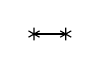
\begin{tikzpicture}[baseline=-3pt]
    \draw [{Rays[n=6]}-{Rays[n=6]}] (0,0) -- (0.55,0);
\end{tikzpicture}
}

\newcommand{\circstar}{% 
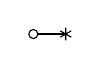
\begin{tikzpicture}
    \draw [{Circle[open]}-{Rays[n=6]}] (0,0) -- (0.55, 0);
\end{tikzpicture}
}

\newcommand{\starcirc}{% 
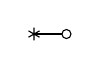
\begin{tikzpicture}
    \draw [{Rays[n=6]}-{Circle[open]}] (0,0) -- (0.55, 0);
\end{tikzpicture}
}

\newcommand{\stararrow}{% 
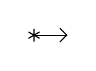
\begin{tikzpicture}
    \draw [{Rays[n=6]}-{Straight Barb[length=2.5pt]}] (0,0) -- (0.5, 0);
\end{tikzpicture}
}

\newcommand{\arrowstar}{% 
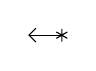
\begin{tikzpicture}
    \draw [{Straight Barb[length=2.5pt]}-{Rays[n=6]}] (0,0) -- (0.5, 0);
\end{tikzpicture}
}

\newcommand{\circarrow}{% 
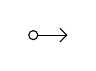
\begin{tikzpicture}
    \draw [{Circle[open]}-{Straight Barb[length=2.5pt]}] (0,0) -- (0.5, 0);
\end{tikzpicture}
}

\newcommand{\tailcirc}{% 
\begin{tikzpicture}[baseline=-3pt] 
    \draw [-{Circle[open]}] (0,0) -- (0.4, 0);
\end{tikzpicture}
}

\newcommand{\circtail}{% 
\begin{tikzpicture}[baseline=-3pt] 
    \draw [{Circle[open]}-] (0,0) -- (0.4, 0);
\end{tikzpicture}
}

\newcommand{\circirc}{% 
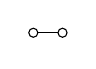
\begin{tikzpicture}[baseline=-3pt] 
    \draw [{Circle[open]}-{Circle[open]}] (0,0) -- (0.5, 0);
\end{tikzpicture}
}

\newcommand{\tailstar}{% 
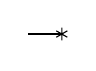
\begin{tikzpicture}[baseline=-3pt] 
    \draw [-{Rays[n=6]}] (0,0) -- (0.5, 0);
\end{tikzpicture}
}

\newcommand{\startail}{% 
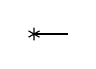
\begin{tikzpicture}
    \draw [{Rays[n=6]}-] (0,0) -- (0.5, 0);
\end{tikzpicture}
}

\newcommand{\tailarrow}{% 
\begin{tikzpicture}
    \draw [-{Straight Barb[length=2.5pt]}](0,0) -- (0.4, 0);
\end{tikzpicture}
}

\newcommand{\arrowtail}{% 
\begin{tikzpicture}
    \draw [{Straight Barb[length=2.5pt]}-](0,0) -- (0.4, 0);
\end{tikzpicture}
}

\newcommand{\arrowarrow}{% 
\begin{tikzpicture}
    \draw [{Straight Barb[length=2.5pt]}-{Straight Barb[length=2.5pt]}](0,0) -- (0.4, 0);
\end{tikzpicture}
}

\newcommand\stackedarrows{%
        \mathrel{\vcenter{\mathsurround0pt
                \ialign{##\crcr
                \noalign{\nointerlineskip}$\arrowtail$\crcr
                \noalign{\nointerlineskip}$\tailarrow$\crcr
                }
        }}%
}
\makeatletter
\@ifpackageloaded{caption}{}{\usepackage{caption}}
\AtBeginDocument{%
\ifdefined\contentsname
  \renewcommand*\contentsname{Table of contents}
\else
  \newcommand\contentsname{Table of contents}
\fi
\ifdefined\listfigurename
  \renewcommand*\listfigurename{List of Figures}
\else
  \newcommand\listfigurename{List of Figures}
\fi
\ifdefined\listtablename
  \renewcommand*\listtablename{List of Tables}
\else
  \newcommand\listtablename{List of Tables}
\fi
\ifdefined\figurename
  \renewcommand*\figurename{Figure}
\else
  \newcommand\figurename{Figure}
\fi
\ifdefined\tablename
  \renewcommand*\tablename{Table}
\else
  \newcommand\tablename{Table}
\fi
}
\@ifpackageloaded{float}{}{\usepackage{float}}
\floatstyle{ruled}
\@ifundefined{c@chapter}{\newfloat{codelisting}{h}{lop}}{\newfloat{codelisting}{h}{lop}[chapter]}
\floatname{codelisting}{Listing}
\newcommand*\listoflistings{\listof{codelisting}{List of Listings}}
\makeatother
\makeatletter
\makeatother
\makeatletter
\@ifpackageloaded{caption}{}{\usepackage{caption}}
\@ifpackageloaded{subcaption}{}{\usepackage{subcaption}}
\makeatother

\ifLuaTeX
  \usepackage{selnolig}  % disable illegal ligatures
\fi
\usepackage{bookmark}

\IfFileExists{xurl.sty}{\usepackage{xurl}}{} % add URL line breaks if available
\urlstyle{same} % disable monospaced font for URLs
\hypersetup{
  pdftitle={Connecting Precariousness and Depression: From Causal Discovery to Intervention Simulation},
  colorlinks=true,
  linkcolor={blue},
  filecolor={Maroon},
  citecolor={Blue},
  urlcolor={Blue},
  pdfcreator={LaTeX via pandoc}}


\title{Connecting Precariousness and Depression: From Causal Discovery
to Intervention Simulation}


\author{%
  %
  %
}


\date{2026-03-16}




\begin{document}
\maketitle
\begin{abstract}
\noindent \textcolor{BrickRed}{Precariousness and depression are closely linked, but the potential causal structure of this relationship and the extent to which feedback between them may shape intervention responses remain unclear. Using cross-sectional data from more than 21,000 adults in the multi-ethnic HELIUS study, we use constraint-based causal discovery methods that allow for latent confounding and feedback to generate hypotheses about candidate graph structures linking precariousness domains and depressive symptoms. Because the data are cross-sectional and many edge orientations are not uniquely determined, we summarize the findings in terms of their stability across specifications and resampling, and treat suggested directions as tentative, data-compatible hypotheses rather than identified causal effects. Across specifications and algorithms, financial stress is the precariousness domain most consistently linked to depression in the causal discovery summaries. Directional edge marks are less stable: in FCI summaries, the edge pattern is more often consistent with financial stress preceding depression, whereas CCI and PC tend to leave the same relation unresolved. In addition, several symptom-level configurations suggest that depressive symptoms may contribute to downstream social precariousness. We then use a calibrated simulation model to examine how depression and precariousness could co-evolve under intervention scenarios across different feedback strengths compatible with the observed data. In the simulation model, slower but more persistent improvement follows intervention under stronger internal feedback, whereas faster but less durable change follows under weaker feedback. These findings suggest that intervention responses may depend not only on the size of the external change but also on the feedback structure linking precariousness and depression. Longitudinal and quasi-experimental studies are needed to clarify directionality, estimate feedback strengths, and assess the policy relevance of these patterns.}
\end{abstract}


\section{Introduction}\label{introduction}

Mental health disorders represent a growing global health concern,
especially in urbanized regions (Gruebner et al., 2017; World Health
Organization, 2022). In 2019, one in eight people worldwide were living
with a mental health condition, with the highest disability-adjusted
life years (DALYs) due to mental and addictive disorders present in
high-income countries such as those in Northern Europe, North America,
and Australia (Rehm \& Shield, 2019; World Health Organization, 2022).
Despite growing awareness, governments have struggled to design
effective responses. Mental health outcomes arise from complex,
multi-level dynamics between the social, economic, and spatial
structures of urban environments---making both diagnosis and
intervention design deeply challenging (Van Der Wal et al., 2021).

Recent work has shifted focus from individual-level vulnerability to
broader social and structural determinants. While high-income nations
show elevated overall DALYs, within-country disparities reveal that
income inequality is a significant predictor of mental health burden
(Rehm \& Shield, 2019). Moreover, precarious working conditions, housing
instability, and neighborhood disadvantage have all been linked to
increased risk of depression and anxiety (Fone et al., 2014; Pevalin et
al., 2017; Rönnblad et al., 2019; Rugulies et al., 2023). This growing
literature highlights that poor mental health is not merely a personal
issue but one rooted in sustained socioeconomic stress and structural
uncertainty.

Building on this, recent studies have introduced the concept of
precariousness as a multidimensional condition characterized by
instability and lack of control across several life domains, including
employment, finances, housing, social relations, and cultural belonging
(Elsenburg et al., 2025; McKee et al., 2017). This broader view reveals
how different forms of insecurity can co-occur and compound, forming an
ecosystem of risk. However, despite growing evidence of association
between precariousness and mental health, a fundamental question remains
unresolved: \emph{How do these factors causally influence one another?}
Most existing studies rely on cross-sectional correlations, leaving open
questions about directionality and
feedback.\footnote{\textcolor{BrickRed}{For conventional effect-size context in HELIUS (e.g., regression-based associations between socioeconomic exposures and depressive symptoms), see the broader HELIUS epidemiologic and measurement literature, for example: Elsenburg et al. (2025), Galenkamp et al. (2017), and Stronks et al. (2013, 2020).}}
Without stronger causal insight, it remains difficult to identify
priority targets for intervention or to anticipate and quantify intended
and unintended effects.

\textcolor{BrickRed}{This study aims to characterize candidate causal structure linking precariousness and depression and to examine how alternative plausible internal configurations could shape responses to stress-reducing scenarios. Specifically, we ask: \textit{How does the internal configuration of the precariousness–depression relationship affect system responses under external reductions in stress?}
To answer this, we combine two approaches. First, we use cycle-capable causal discovery algorithms to infer equivalence-class constraints among domain-specific precariousness factors and depressive symptoms under possible latent confounding and feedback.
By examining both aggregated measures (depression sum score and a composite precariousness index) and disaggregated variables (individual depressive symptoms and specific life-domain indicators), we capture broad patterns of conditional dependence as well as finer-grained candidate pathways.
Second, we translate the most stable motifs and remaining uncertainty into a deliberately simplified dynamical model that simulates how depression and precariousness could co-evolve under external stress reduction.
This model is used as a scenario tool to probe how system properties—especially feedback strength—can shape the speed and persistence of response. For example, when feedback from precariousness to depression is weaker, depression responds more directly to stress reduction but can also rebound more quickly when stress is reintroduced; when feedback is stronger, responses can be slower but more persistent.}

\textcolor{BrickRed}{In much of the public health and social epidemiology literature, analyses of precariousness and depression necessarily rely on associational summaries (e.g., regressions or correlations), even when the substantive discussion is implicitly causal in terms of drivers, upstream factors, or mutual reinforcement. Our goal is to show what additional structural and uncertainty information becomes visible when one uses causal-structure learning outputs and then carries those insights forward into scenario-based simulations, rather than implicitly treating one fitted model as “the” causal story.}

\textcolor{BrickRed}{Because HELIUS is cross-sectional and many orientations are unstable across algorithms and CI tests, we do not treat the discovery output as identifying a unique mechanism of mutual reinforcement. Instead, we use causal discovery to summarize which adjacencies and motifs are stable versus indeterminate, and we carry the remaining uncertainty forward into scenario simulations that illustrate how different plausible feedback regimes could shape intervention trajectories.}
\textcolor{BrickRed}{Our contribution is primarily integrative. We provide an applied workflow that (i) estimates candidate structural constraints among precariousness and depression under latent confounding and possible feedback, (ii) makes uncertainty explicit via resampling and a prespecified specification grid, and (iii) carries the stable motifs and remaining uncertainty forward into scenario simulations rather than fixing a single directed graph.}

\section{Methods}\label{methods}

\subsection{Data}\label{data}

We use data from the HELIUS (HEalthy LIfe in an Urban Setting) study
(Snijder et al., 2017; Stronks et al., 2013). It captures the diverse
population of the city of Amsterdam by including the six main ethnic
groups and provides comprehensive health and lifestyle data, including
depressive symptoms as measured by the PHQ-9 (Galenkamp et al., 2017).
\textcolor{BrickRed}{To operationalize precariousness, we follow the domain framework described in prior work}
(Elsenburg et al., 2025)
\textcolor{BrickRed}{and compile candidate indicators for each domain. Before entering the causal discovery pipeline, we screened these candidates for measurement quality and within-domain coherence among the precariousness indicators (e.g., missingness, variability, and inter-item correlations). 
This resulted in five precariousness factors: three structural domains (employment, housing, and social relationships) and two domains capturing recent life stressors (financial and relational). Each factor is composed of multiple observed variables, as outlined below. Additional details on the HELIUS study and the factor extraction process are provided in the}
\hyperref[sec-appendix]{Appendix}.

\begin{itemize}
\tightlist
\item
  Employment precariousness: \texttt{emp\_stat} (current employment
  status), \texttt{work\_sit} (nature of work situation).
\item
  Social precariousness: \texttt{soc\_freq} (frequency of social
  contact), \texttt{soc\_adq} (perceived adequacy of social support).
\item
  Housing precariousness: \texttt{nb\_safe} (neighborhood safety),
  \texttt{nb\_res} (access to neighborhood resources), \texttt{nb\_rent}
  (proportion of rental housing), \texttt{cul\_rec} (availability of
  cultural resources).
\item
  Recent relational stressors: \texttt{frd\_brk12} (experience of a
  friendship breakup), \texttt{conf12} (recent interpersonal or
  relational conflict).
\item
  Recent financial stressors: \texttt{fincri12} (experience of a
  financial crisis), \texttt{inc\_dif} (difficulty managing household
  income).
\end{itemize}

Following data cleaning and normalization procedures, the analytical
sample comprises 21,628 individuals.
\textcolor{BrickRed}{Because participation and item nonresponse may be selective, and because the analytic sample excludes individuals with missing data on key variables, the observed associations may, in principle, partly reflect selection mechanisms in addition to population-level relationships.}
In addition to the five identified precariousness factors, we computed
an overall precariousness score by summing these five factor scores,
thereby capturing a composite measure of accumulated precariousness
across domains.

\textcolor{BrickRed}{In the causal-discovery analyses, recent financial stressors (\textit{S.fin}), social precariousness (\textit{P.soc}), and the overall precariousness score are treated as measured proxies for broader underlying conditions that may be influenced by policy or program levers. For example, \textit{S.fin} may reflect acute financial strain that could in principle be shifted by income support, debt relief, bill assistance, or related forms of financial support; \textit{P.soc} may reflect social connectedness and barriers to participation that could in principle be shifted by social support or access-enhancing interventions; and the overall precariousness score is interpreted as a composite proxy for accumulated disadvantage across domains rather than as a single directly manipulable target. Interpreting changes in these proxy measures as policy-relevant shifts requires additional assumptions: (i) the intervention produces a stable change in the proxy as measured; (ii) the proxy is measured comparably across relevant groups and settings; (iii) the intervention does not have large effects on depression through pathways that bypass the targeted proxy; and (iv) a given change in the proxy corresponds to a meaningful change in the target construct it is intended to represent. In the simulation analyses, however, the only externally implemented intervention is a reduction in the financial stress proxy; depression and social precariousness evolve endogenously through the model couplings.}

Depression is represented using the PHQ-9 (Kroenke et al., 2001), both
as a total sum score and as individual symptom scores. In the subsequent
causal discovery analysis, we explore the relationship between
depression and precariousness using both aggregated scores and their
disaggregated components. See Figure~\ref{fig-dist} for the overall
distributions of the variables used in the analysis.

\begin{figure}

\centering{


\includegraphics[width=0.9\textwidth,height=\textheight]{draft_v3_SSM_anonymized_LE_KS_files/figure-pdf/fig-dist-1.pdf}

}

\caption{\label{fig-dist}\textbf{\emph{Distributions of variables with
density overlay.}} This shows the distributions of the variables used in
the causal analysis, plotted as histograms with overlaid density
estimates. The x-axis represents the value of each variable after
preprocessing. The y-axis shows the corresponding estimated probability
density. \textbf{\emph{P.emp}} = \emph{employment precariousness};
\textbf{\emph{P.hou}} = \emph{housing precariousness};
\textbf{\emph{P.soc}} = \emph{social precariousness};
\textbf{\emph{S.fin}} = \emph{recent financial stressors};
\textbf{\emph{S.rel}} = \emph{recent relational stressors};
\textbf{\emph{precariousness}} = \emph{overall precariousness};
\textbf{\emph{PHQsum}} = \emph{PHQ-9 sum score}; \textbf{\emph{anh}} =
\emph{anhedonia}; \textbf{\emph{app}} = \emph{appetite};
\textbf{\emph{con}} = \emph{concentration}; \textbf{\emph{dep}} =
\emph{depressed mood}; \textbf{\emph{ene}} = \emph{energy};
\textbf{\emph{glt}} = \emph{guilty}; \textbf{\emph{mot}} = \emph{motor};
\textbf{\emph{slp}} = \emph{sleep}; \textbf{\emph{sui}} =
\emph{suicidal}.}

\end{figure}%

\subsection{Causal Discovery}\label{sec-analysis}

\textcolor{BrickRed}{To characterize candidate causal structures and obtain constraints on possible ancestral relations between precariousness and depression, we use constraint-based causal discovery algorithms that allow for feedback loops and latent confounding.}
Specifically, we apply the \emph{Fast Causal Inference} (FCI) and
\emph{Cyclic Causal Inference} (CCI) algorithms,
\textcolor{BrickRed}{both of which allow latent confounding and can represent certain classes of feedback/cyclicity under additional assumptions}
(Mooij \& Claassen, 2020; Strobl, 2019). For reference, we also include
the \emph{PC} algorithm, one of the most widely used methods for acyclic
causal discovery (Spirtes et al., 2001). While our full analysis
includes results from three causal discovery algorithms---FCI, CCI, and
PC---we focus on FCI in the main text, as it offers a strong balance
between flexibility and theoretical soundness.
\textcolor{BrickRed}{FCI accommodates latent confounding and can represent certain classes of feedback under additional assumptions/extensions, making it well-suited for the complexity of our data}
(Mooij \& Claassen, 2020). The PC algorithm is included for reference
but relies on more restrictive assumptions, such as acyclicity and no
unmeasured confounding. CCI, while capable of modeling cycles
explicitly, has its own theoretical limitations; for example, its output
may not fully preserve the d-separation properties of the true causal
graph (Strobl, 2019). Results from both PC and CCI are provided in the
\hyperref[sec-appendix]{Appendix}
(Section~\ref{sec-cci}, Section~\ref{sec-pc}) for completeness and
comparison. For readers interested in detailed explanations of the
algorithms, edge interpretations, and graph types (e.g., PAG, MAAG,
CPDAG), as well as algorithmic assumptions and limitations, please refer
to the \hyperref[sec-appendix]{Appendix}
(Section~\ref{sec-causalprimer})\textcolor{BrickRed}{; a more tutorial-style walkthrough with simulations is provided in}
Park et al. (2024).
\textcolor{BrickRed}{These discovery procedures do not explicitly model participation or missingness mechanisms. We therefore interpret inferred adjacencies as conditional on the analyzed sample, and selection-induced associations cannot be ruled out without additional information about the selection process.}

\textcolor{BrickRed}{The output of these algorithms is interpreted as an equivalence-class summary of edge marks compatible with the conditional independencies observed in the data under stated assumptions. That is, the algorithms do not identify a single causal graph; rather, they return a class of graphs compatible with the data, and the endpoint marks indicate which possible ancestral relations are constrained and which remain unresolved. In cross-sectional settings with measurement error and finite samples, edge orientations are often not uniquely determined and may vary across algorithms, conditional independence tests, and resampling. We therefore interpret stable adjacencies (link existence) as consistently recovered links under the tested specifications and treat edge orientations as hypothesis-generating rather than as identified directionality or causal effects.}

A key challenge in applying these algorithms to the HELIUS dataset is
that many variables are non-Gaussian and likely exhibit nonlinear
relationships. While kernel-based conditional independence tests (such
as KCIT) are well-suited for capturing such complex dependencies, they
are computationally intensive---scaling quadratically with sample size
due to the need to invert large kernel matrices---making them
impractical for large datasets like HELIUS (Rahimi \& Recht, 2007). To
address this, we use the Randomized Conditional Correlation Test (RCoT),
a
\textcolor{BrickRed}{scalable nonparametric alternative that approximates kernel methods using random Fourier features, replacing expensive kernel-matrix computations with lower-dimensional feature operations and thereby substantially reducing runtime at large sample sizes}
(Strobl et al., 2019; Zhang et al., 2011).
\textcolor{BrickRed}{RCoT improves computational feasibility relative to KCIT and allows sensitivity analyses at HELIUS sample size, but it does not remove the fundamental loss of statistical power that typically occurs as the conditioning set size $|Z|$ increases.}
For further details, see Section~\ref{sec-rcot}.

We examine the causal structure using three complementary approaches:

\begin{enumerate}
\def\labelenumi{\arabic{enumi}.}
\tightlist
\item
  Aggregate-level analysis: relationships between five domain-specific
  precariousness factors and the PHQ-9 sum score.
\item
  Fully disaggregated analysis: relationships between individual
  precariousness items and individual depressive symptoms.
\item
  Mixed analysis: relationships between individual symptoms and a
  composite index of overall precariousness.
\end{enumerate}

The aggregate analysis reduces dimensionality and yields interpretable
summaries of how domains of precariousness relate to overall depression
severity. However, it may obscure finer-grained effects. The
disaggregated analysis allows for precise mapping of which symptoms are
influenced by (or influence) specific precariousness conditions, but it
introduces complexity due to the high dimensionality and distributional
properties of the data. The mixed approach, in turn, integrates these
perspectives by examining how individual symptoms respond to cumulative
precariousness across domains.

\textcolor{BrickRed}{To summarize the stability of the estimated graph structure between depression and precariousness variables, we implement a comprehensive bootstrapped causal discovery procedure.}
This procedure systematically varies key analysis parameters across a
grid of configurations, enabling us to assess the stability of inferred
relationships under different settings. Specifically, we vary four main
components:

\begin{itemize}
\tightlist
\item
  Significance levels for conditional independence tests: \(\alpha\) =
  0.01 and 0.05.
\item
  Stability thresholds: 0.5, 0.6, 0.7, and 0.8, which determine how
  frequently an edge must appear across bootstraps to be retained.
\item
  Conditional independence (CI) tests: Gaussian CI test (partial
  correlation) and RCoT (a nonparametric test).
\item
  Causal discovery algorithms: FCI, CCI, and PC.
\end{itemize}

For each unique parameter combination (2 significance levels × 4
thresholds × 2 CI tests = 16 settings), we run 100 bootstrap samples per
algorithm for the aggregated analyses (see Step 1 in
Figure~\ref{fig-workflow}). For symptom-level analyses, which are more
computationally intensive, we use 30 bootstrap samples per
setting.\footnote{For symptom-level analyses, we further improve
  computational efficiency by fixing the skeleton structure---the
  undirected network of potential connections---using a consensus graph
  derived from all three algorithms (with \(\alpha = 0.01\) and the RCoT
  test). This allows subsequent analyses to focus exclusively on
  estimating edge directions, avoiding the repeated and costly
  computation of skeletons, and thus substantially reducing runtime.}

To summarize these results, we apply a two-level aggregation strategy:

\begin{enumerate}
\def\labelenumi{\arabic{enumi}.}
\tightlist
\item
  \textbf{Within each condition} (fixed \(\alpha\), threshold, CI test,
  and algorithm), we identify the most frequently occurring edge type
  (e.g., arrowhead, circle, none) across bootstraps for each pair of
  variables (Step 2 in Figure~\ref{fig-workflow}).
\item
  \textbf{Across conditions},
  \textcolor{BrickRed}{we summarize edge marks by their most frequent edge mark across the specification grid. If two or more edge marks are tied for the highest frequency, we label the edge as uncertain and draw it as dashed in the final graph}
  (Step 3 in Figure~\ref{fig-workflow}).
  \textcolor{BrickRed}{Dashed edges therefore indicate indeterminacy across specifications and are not treated as directionally informative.}
\end{enumerate}

This summarization process is repeated separately for each causal
discovery algorithm (FCI, CCI, PC),
\textcolor{BrickRed}{yielding a single summary graph per algorithm. These final graphs represent only the most stable and consistent relationships across a wide range of plausible parameterizations, improving interpretability and making sensitivity to analysis choices explicit.}
To support transparency, each final graph is accompanied by a matrix
summarizing the relative frequency of each edge type for every variable
pair, enabling readers to assess the degree of uncertainty or agreement
underlying each connection.

\textcolor{BrickRed}{The purpose of this pipeline is not to produce a single definitive causal graph, but to make sensitivity to modeling choices explicit. Accordingly, the summaries can yield absent edges and indeterminate endpoint marks (ties/dashed edges). We treat these outcomes as substantive indicators of limited information in the data and refrain from resolving them by selecting a preferred specification.}

\textcolor{BrickRed}{Our procedure is intended to summarize how sensitive the estimated graphs are to bootstrap resampling and to a prespecified set of analytic choices. The bootstrap-based edge-type proportions are interpreted as descriptive relative frequencies of returned edge marks. That is, they summarize how often a given edge mark is returned across bootstrap resamples and specifications, rather than providing hypothesis-test p-values or a formal statistical guarantee. We treat stability as a descriptive property with two components. First, \emph{adjacency stability} refers to how consistently an edge is recovered across bootstrap resamples and specifications. Second, \emph{orientation stability} refers to how consistently the same endpoint-mark pattern is recovered when an adjacency is present.}

\textcolor{BrickRed}{We consider the analysis to show limited stability under any of the following failure modes: (i) an adjacency appears only under a narrow subset of specifications (for example, only at one significance level or only for one CI test); (ii) an adjacency is frequently absent under small changes in the specification grid; or (iii) an orientation is inconsistent across specifications, including frequent reversals between $X \rightarrow Y$ and $Y \rightarrow X$, or a large share of undetermined endpoint marks. In these cases we report the adjacency as unstable or the direction as indeterminate (for example, using dashed edges for ties) and we do not treat the direction as evidence for a causal ordering.}

\begin{figure}

\centering{

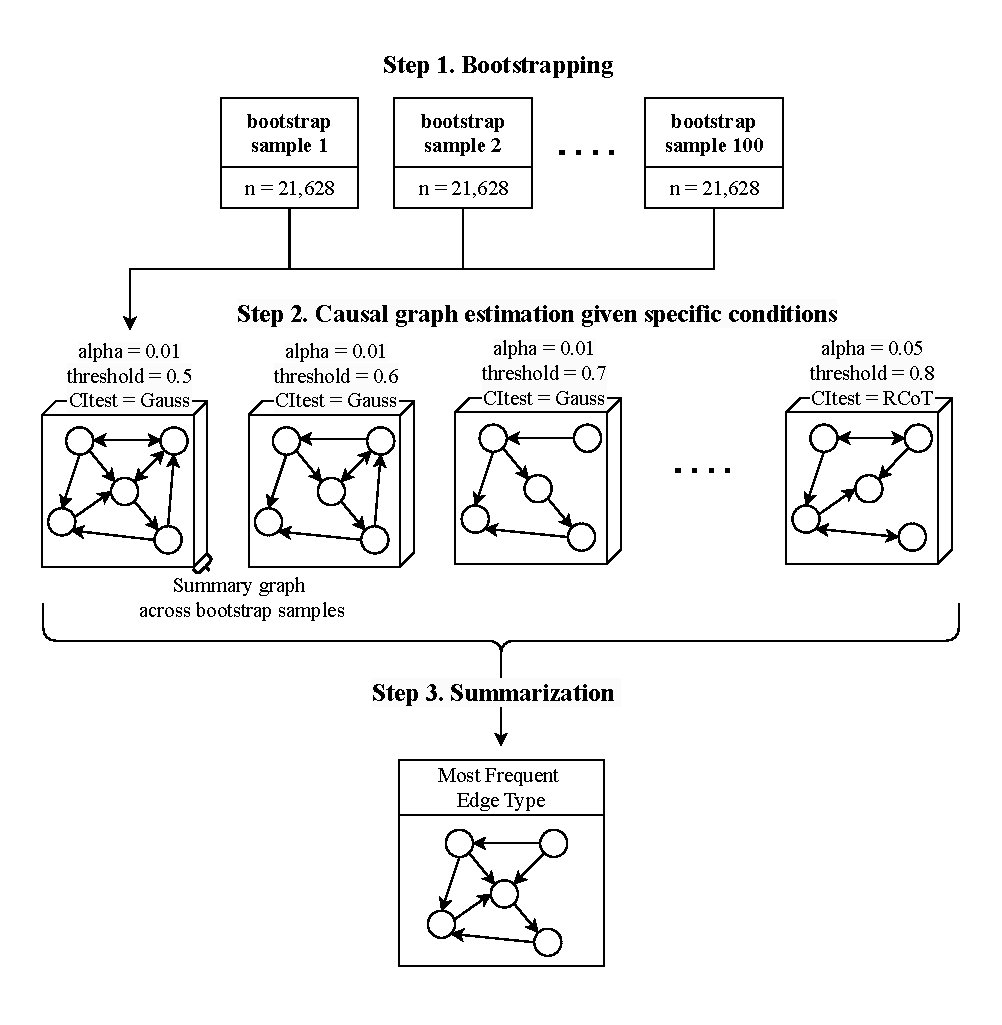
\includegraphics[width=0.9\textwidth,height=\textheight]{img/simsetup.pdf}

}

\caption{\label{fig-workflow}\textbf{\emph{Causal discovery workflow
applied across all three algorithms (FCI, CCI, and PC)}}. The process
involves three main steps: (1) bootstrapping the dataset to create
multiple resampled datasets; (2) estimating causal graphs under varying
parameter configurations; and (3) summarizing results by identifying the
most frequent edge type across bootstraps and settings to construct a
final stable graph.}

\end{figure}%

\subsection{Modeling Dynamics between Precariousness and
Depression}\label{modeling-dynamics-between-precariousness-and-depression}

To explore how internal system structure shapes responses to external
support, we implement a high-level computational model that formalizes
\textcolor{BrickRed}{core motifs highlighted by the causal discovery analysis}.
Rather than attempting to replicate the full estimated causal graph,
this model abstracts the essential structure into a compact, tractable
system focused on dynamic interactions between depression and social
precariousness, both influenced by financial stress.
\textcolor{BrickRed}{The dynamical model is intentionally reduced and should be read as a scenario model anchored to the most stable cross-specification motifs (in particular, the \textit{S.fin}--depression--\textit{P.soc} motif), rather than as a dynamical implementation of the full estimated graph. This reduction is motivated by the discovery results themselves: beyond a small number of recurring adjacencies, many endpoint marks are unstable or method-dependent in this cross-sectional setting, so translating the full graph would risk hard-coding directions that are not stably supported across specifications.}\footnote{\textcolor{BrickRed}{
Because the graph-learning outputs are defined by conditional-independence constraints, whereas our dynamical calibration matches second-order moments (variances/covariances), the scenario model is not expected to reproduce the full PAG/MAAG conditional-independence structure, and we do not interpret it as such.}}
\textcolor{BrickRed}{We use a linear stochastic differential equation model as a transparent baseline scenario; nonlinear threshold mechanisms (e.g., sigmoidal or state-dependent coupling) are not included here because they introduce additional functional-form parameters that are weakly constrained by the cross-sectional data, and we discuss them as a natural extension.}

As illustrated in Figure~\ref{fig-concept}, the model includes three
components: social precariousness \(P_i(t)\), depressive symptoms
\(D_i(t)\), and a static individual-specific external stressor \(S_i\),
representing financial stress. Depression and precariousness are modeled
as coupled state variables that influence each other over time, with
\(S_i\) acting as a shared input. These dynamics are formalized as a
pair of linear stochastic differential equations (SDEs):

\[
\begin{aligned}
dP_i(t) &= \lambda_P \big( \alpha_{PS} S_i + \alpha_{PD} D_i(t) - P_i(t) \big) \, dt + \sigma_P \, dW_{P,i}(t) \\
dD_i(t) &= \lambda_D \big( \alpha_{DS} S_i + \alpha_{DP} P_i(t) - D_i(t) \big) \, dt + \sigma_D \, dW_{D,i}(t)
\end{aligned}
\]

Here, \(D_i(t)\) denotes the depressive state and \(P_i(t)\) denotes the
level of social precariousness for individual \(i\) at time \(t\), with
\(S_i\) representing a static, individual-specific external stressor
(financial stress). The parameters \(\lambda_D\), \(\lambda_P\), as well
as the coefficients \(\alpha\) and noise terms \(\sigma\), are assumed
to be constant across individuals and time. The parameters \(\lambda_D\)
and \(\lambda_P\) govern the timescales over which \(D_i(t)\) and
\(P_i(t)\) adjust toward their respective input-driven target states.
The coefficients \(\alpha_{DS}\) and \(\alpha_{PS}\) quantify the direct
effects of the external stressor \(S_i\) on depression and
precariousness, respectively, while \(\alpha_{DP}\) and \(\alpha_{PD}\)
capture the mutual influence between the two dynamic processes.
Stochastic fluctuations are introduced via the independent Wiener
processes \(dW_{D,i}(t)\) and \(dW_{P,i}(t)\), scaled by their
respective volatility parameters \(\sigma_D\) and \(\sigma_P\). This
linear structure offers a transparent and analytically tractable
framework for modeling how exogenous variation in financial stress may
propagate through individual dynamics of depression and precariousness.
\textcolor{BrickRed}{Under a stationarity assumption, the model can be calibrated to match empirical second-order moments (variances and covariances). Because feedback strength is not uniquely identified from cross-sectional data and can remain difficult to identify even with longitudinal data when time resolution is limited or measurement error is substantial, we treat $\alpha_{DP}$ as a free parameter and derive the remaining coefficients analytically conditional on $\alpha_{DP}$. We then vary $\alpha_{DP}$ over its admissible range and interpret the resulting family of models as a sensitivity analysis.}
The resulting steady-state distribution of the model aligns with
empirical measures: PHQ-9 total score (PHQsum) for depression, and the
derived social precariousness factor (P.soc) for social precarity. The
full calibration procedure is described in
Section~\ref{sec-calibration}.

\begin{figure}

\centering{

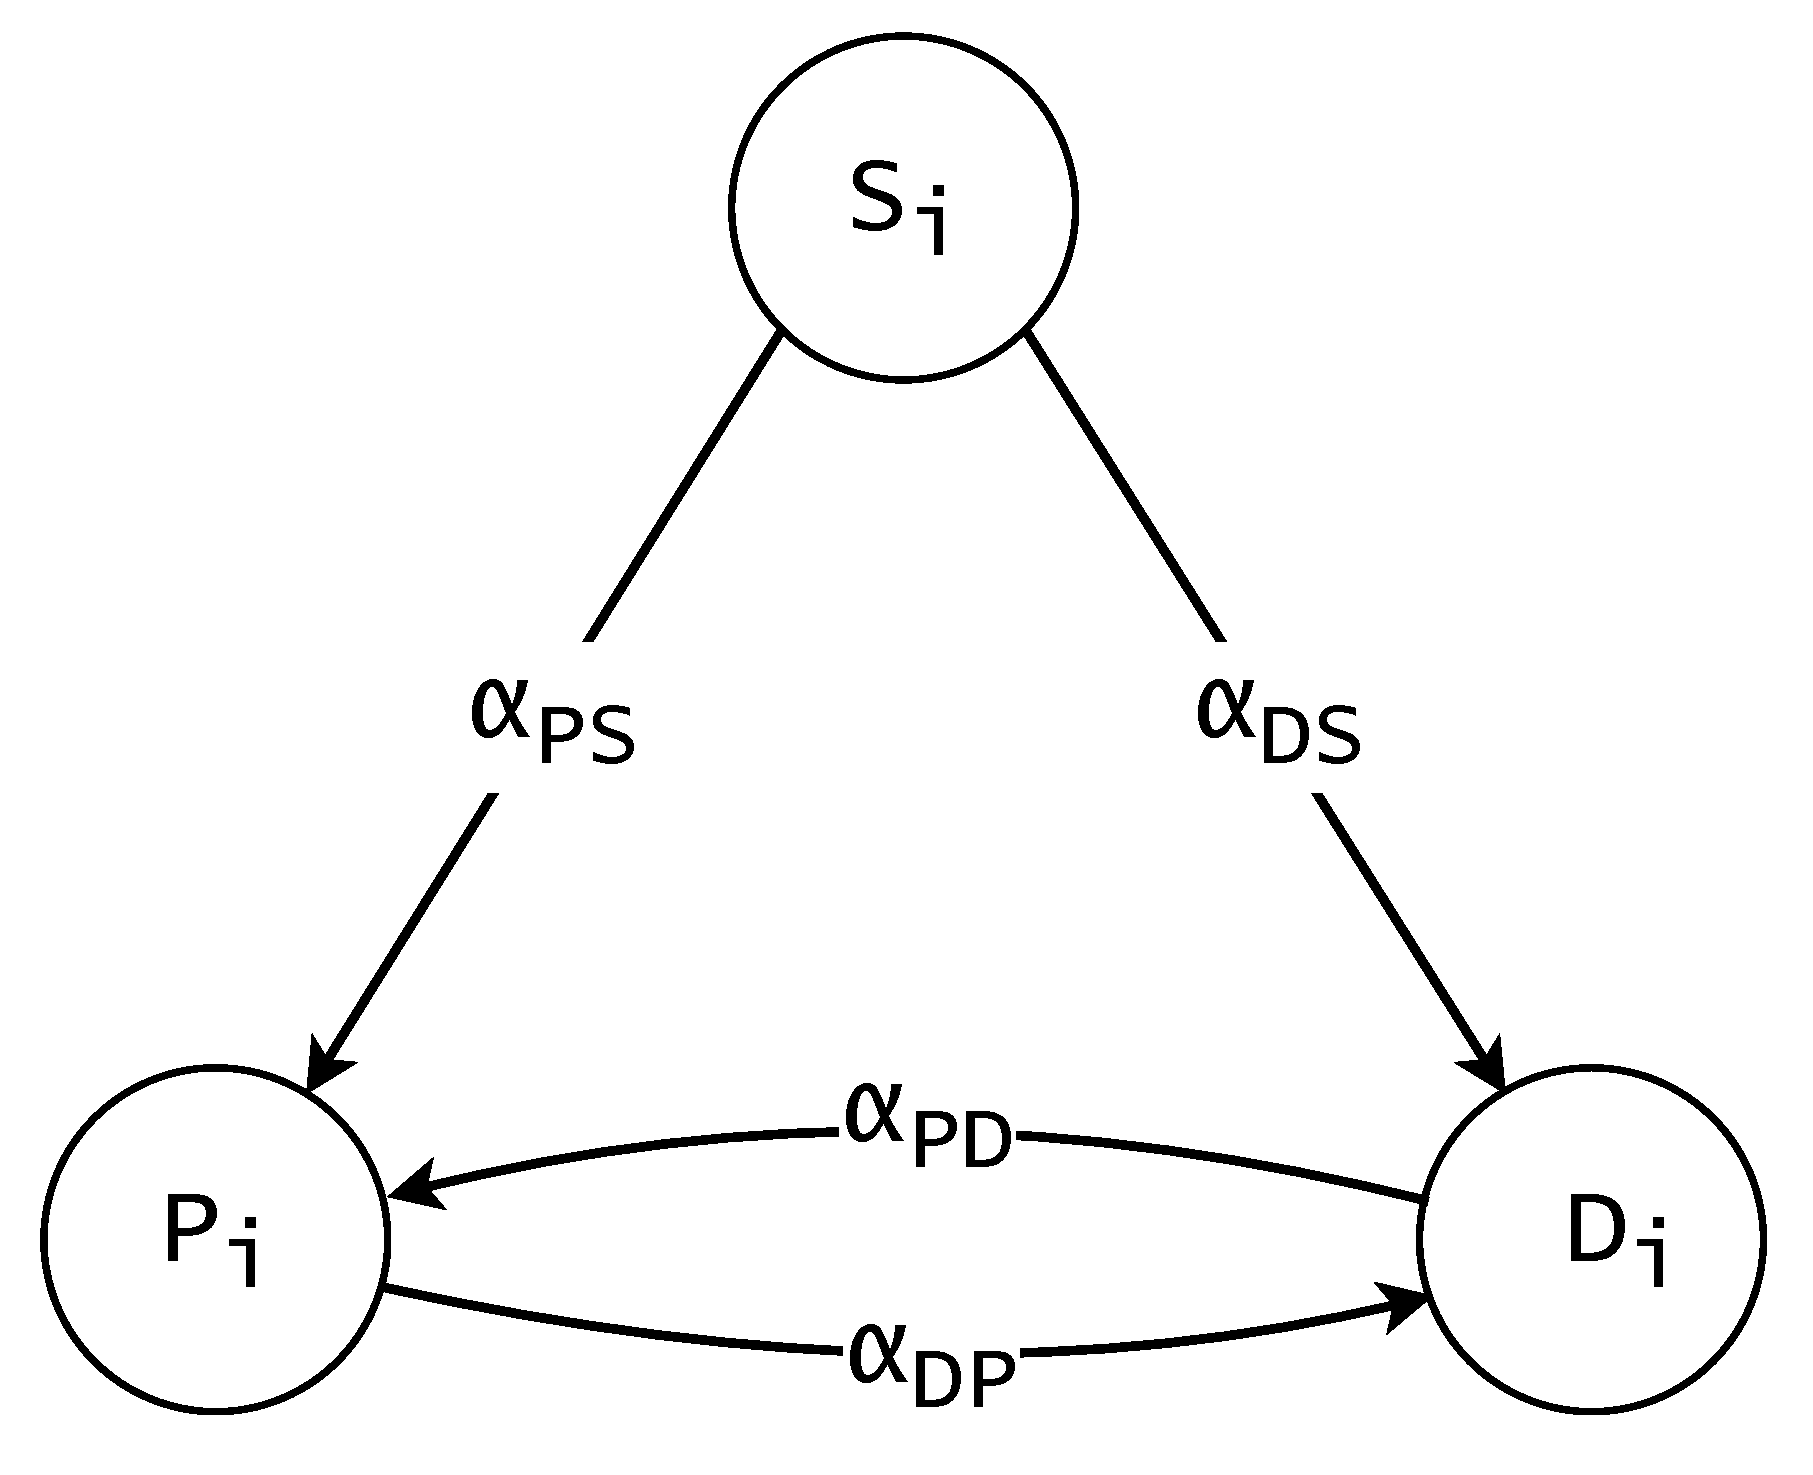
\includegraphics[width=0.4\textwidth,height=\textheight]{img/conceptmodel.pdf}

}

\caption{\label{fig-concept}\textbf{\emph{High-level schematic of the
dynamic model structure used in simulation.}} Arrows represent influence
coefficients \(\alpha\), corresponding to the terms in the system of
stochastic differential equations. \(D_i(t)\) and \(P_i(t)\) denote
depressive symptoms and social precariousness for individual \(i\), with
\(S_i\) representing static financial stress.
\textcolor{BrickRed}{In the simulation model, financial stress is specified as an external input to both depressive symptoms and social precariousness, and depression and precariousness are specified to be mutually coupled.}
Arrows depict influence pathways that are operationalized in our
quantitative model.
\textcolor{BrickRed}{This abstraction is informed by the causal discovery results and provides the structure for the simulation experiments.}}

\end{figure}%

\subsubsection{Model Calibration}\label{sec-calibration}

In our linear model, all parameters are derived analytically to
reproduce the empirical second-order moments observed in the HELIUS
dataset. The system treats depression (\(D\)) and social precariousness
(\(P\)) as jointly evolving under the influence of a shared external
stressor (\(S\)), forming a coupled system of Ornstein--Uhlenbeck
processes. Under the assumption of stationarity, the steady-state
covariances between these variables admit closed-form solutions for the
system's structural parameters.

We fix the adjustment rates \(\lambda_D = \lambda_P = 1\), which
normalizes the time scale given the cross-sectional nature of the HELIUS
data. To resolve the remaining degree of freedom, we treat the feedback
from precariousness to depression (\(\alpha_{DP}\)) as a free parameter,
and we solve algebraically for all other coefficients --- specifically
the direct effects of stress (\(\alpha_{DS}, \alpha_{PS}\)), the reverse
feedback from depression to precariousness (\(\alpha_{PD}\)), and the
noise terms (\(\sigma_D, \sigma_P\)). These solutions are expressed as
closed-form functions of the empirical covariances: \(\mathrm{Var}(D)\),
\(\mathrm{Var}(P)\), \(\mathrm{Var}(S)\), \(\mathrm{Cov}(D, P)\),
\(\mathrm{Cov}(D, S)\), and \(\mathrm{Cov}(P, S)\).

This structure creates a family of analytically calibrated models, each
consistent with the same observed covariances but differing in their
internal configuration. We constrain the space of valid solutions by
imposing that all structural parameters must be positive, reflecting the
assumption that stress and precariousness contribute adversely to
depression. This constraint restricts the allowable range of
\(\alpha_{DP}\) to approximately \([0, 0.698]\) (see Appendix
Section~\ref{sec-analcalibration}).

Figure~\ref{fig-tradeoff} illustrates how the remaining parameters
adjust as \(\alpha_{DP}\) increases to maintain consistency with the
empirical covariances. As \(\alpha_{DP}\) increases, \(\alpha_{PD}\)
tends to decrease, reflecting a compensatory trade-off between the
mutual influences of depression and precariousness. This interplay helps
preserve the model's match with observed covariances, without requiring
major shifts in external input strength. Meanwhile, the external
coupling terms --- \(\alpha_{DS}\) and \(\alpha_{PS}\) --- also shift to
absorb variance in a way that maintains alignment with the empirical
data. Notably, the noise amplitudes \(\sigma_D\) and \(\sigma_P\)
decline slightly as \(\alpha_{DP}\) increases. This indicates that more
of the observed variability is captured by deterministic interactions,
with less left to be explained by stochastic fluctuations.

\textcolor{BrickRed}{This remaining flexibility reflects non-identifiability of feedback strength in cross-sectional data. We therefore treat the resulting one-parameter family as a sensitivity analysis: each member matches the same empirical covariance structure, but differs in internal feedback configuration, allowing us to examine how intervention trajectories depend on plausible feedback regimes.}
Each represents a different plausible causal architecture, offering
insight into how internal dynamics modulate the system's responsiveness
to external stress --- even when the observed covariances remain
unchanged.

\begin{figure}

\centering{

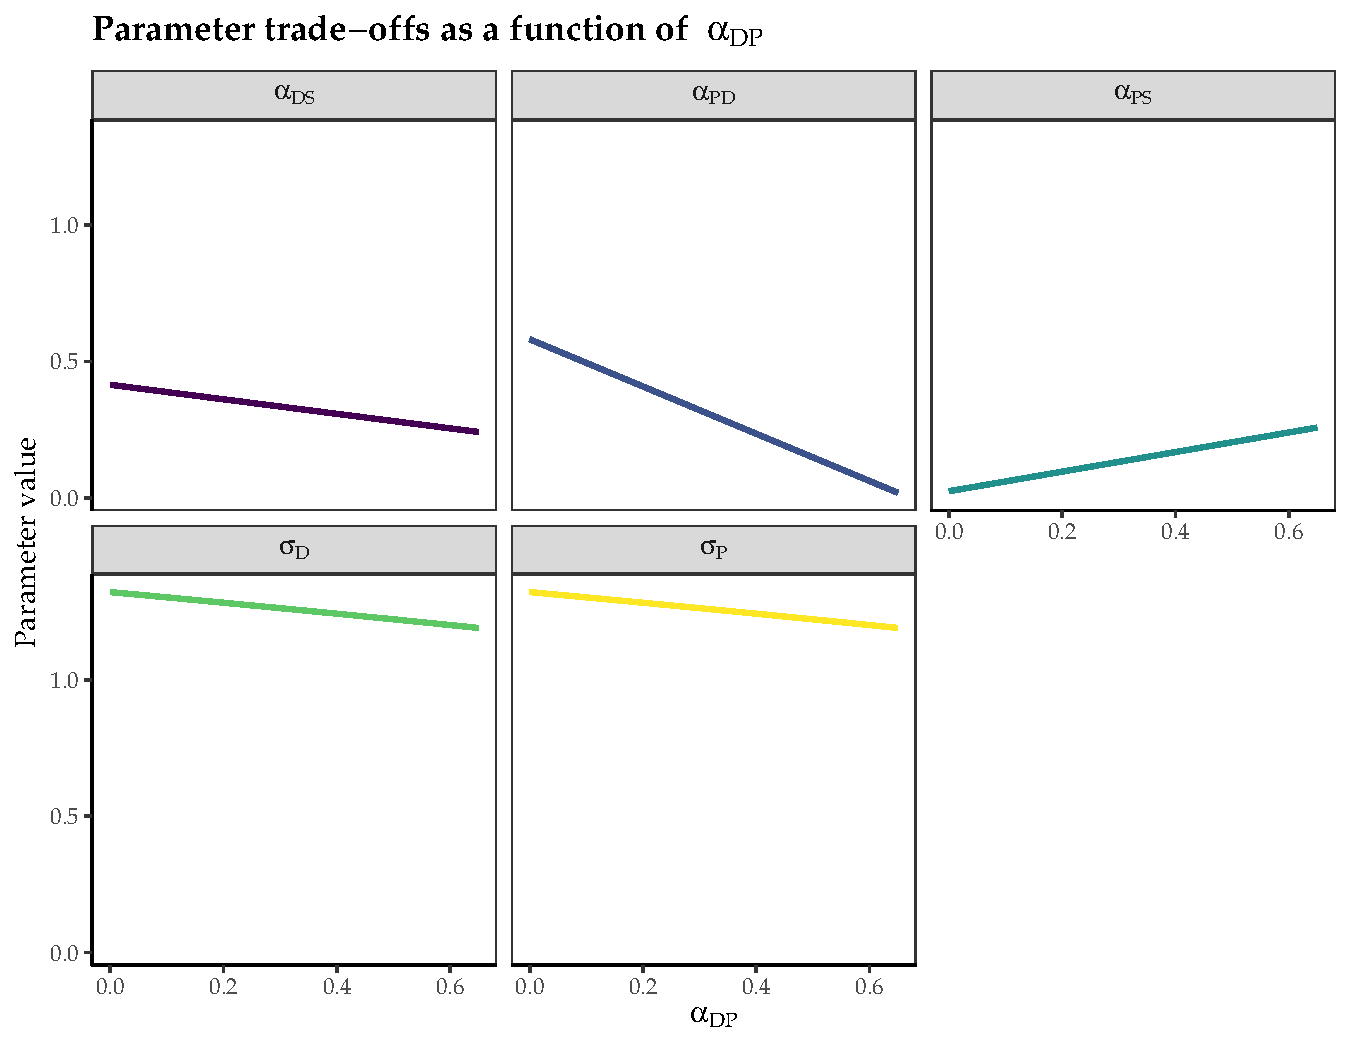
\includegraphics[width=0.85\textwidth,height=\textheight]{img/param_tradeoff.pdf}

}

\caption{\label{fig-tradeoff}\textbf{\emph{Trade-off curves showing how
calibrated parameters vary with coupling strength.}} Each line tracks
how a model parameter changes with the coupling coefficient
(\(\alpha_{DP}\)), which quantifies the influence of precariousness on
depression in the dynamical model. These adjustments preserve
consistency with empirical covariances from the HELIUS data. Together,
the curves illustrate that multiple internal configurations are equally
compatible with the data, highlighting how system dynamics can
reorganize as coupling strength varies.}

\end{figure}%

\subsubsection{Intervention Simulation}\label{intervention-simulation}

To evaluate how internal structure affects system responsiveness, we
simulate a family of linear models under an external support scenario.
Each model corresponds to a different value of \(\alpha_{DP}\),
representing the strength of influence from social precariousness to
depression. The range spans from 0 (no coupling) to 0.65 (maximal
admissible value), with all other parameters derived analytically to
preserve the empirical covariances observed in the HELIUS data (see
Figure~\ref{fig-tradeoff}).

\textcolor{BrickRed}{In each simulation, we represent external support by shifting the financial stress proxy for individual $i$ ($S_i$) downward by a common proportion toward the lowest observed value in the cohort. This is a stylized representation of stress-reducing policies that are expected to lower acute financial strain (for example, income support or benefits, debt relief, or related forms of financial assistance). We do not intervene directly on depression $D_i(t)$ or social precariousness $P_i(t)$. Instead, $D_i(t)$ and $P_i(t)$ evolve endogenously in response to the change in $S_i$ through the model couplings. We simulate 1000 virtual individuals per model, sampling baseline stress levels from the empirical distribution and lowering those levels by the same proportion (intervention level).}

We assess the system's behavior using two complementary approaches:

\begin{itemize}
\item
  Snapshot analysis captures the average levels of depression (\(D\))
  and precariousness (\(P\)) at selected time points (\(t = 100\),
  \(300\), \(500\)) following intervention onset. Since all linear
  models converge to the same equilibrium, this highlights how internal
  feedback affects the speed and pathway of adjustment.
\item
  Full trajectory simulation tracks system dynamics over time for two
  representative models: one with minimal (\(\alpha_{DP} = 0\)) and one
  with maximal (\(\alpha_{DP} = 0.65\)) feedback. Each simulation
  includes an intervention period followed by its withdrawal, revealing
  differences in reactivity, delay, and recovery stability.
\end{itemize}

Together, these simulations demonstrate how internal structure governs
not just whether change occurs, but how it unfolds --- shaping the pace,
persistence, and variability of response to external support.

\section{Results}\label{results}

\subsection{Causal Structure Linking Precariousness and
Depression}\label{causal-structure-linking-precariousness-and-depression}

\textcolor{BrickRed}{Because the estimated graphs are equivalence-class outputs and HELIUS is cross-sectional, we use these results to generate hypotheses rather than to identify causal effects. We distinguish adjacency stability, meaning whether a connection is repeatedly recovered, from orientation stability, meaning how consistently endpoint marks suggest the same possible direction across specifications. Unresolved orientations are treated as indeterminacy rather than as evidence for or against a directional effect. When stability is limited, we report the relation as indeterminate and refrain from directional interpretation.}

\begin{abbrbox}
\textbf{Abbreviations used in Results.}
\emph{P.emp} = employment precariousness; \emph{P.hou} = housing precariousness; \emph{P.soc} = social precariousness; \emph{S.fin} = recent financial stressors; \emph{S.rel} = recent relational stressors; \emph{PHQsum} = PHQ-9 sum score; \emph{anh} = anhedonia; \emph{app} = appetite; \emph{con} = concentration; \emph{dep} = depressed mood; \emph{ene} = energy; \emph{glt} = guilt; \emph{mot} = psychomotor change; \emph{slp} = sleep disturbance; \emph{sui} = suicidal ideation.
\end{abbrbox}

\subsubsection{Depression as sum score}\label{depression-as-sum-score}

Figure~\ref{fig-sum} provides a summary of how precariousness factors
collectively influence and are influenced by overall depression
severity,
\textcolor{BrickRed}{focusing on the estimated graph structure between precariousness factors (\textit{P.hou, P.emp, P.soc, S.rel, S.fin}) and the depression sum score (PHQsum), as returned by the FCI algorithm.}

\textcolor{BrickRed}{In panel (a) we see that employment precariousness (\textit{P.emp}) and social precariousness (\textit{P.soc}) are adjacent to PHQsum, but their endpoint marks do not consistently support an interpretation in which they precede depression; in fact, the most frequent patterns are often unresolved or oriented in the opposite direction. By contrast, financial stress (\textit{S.fin}) shows the most stable adjacency with \textit{PHQsum} and is more often oriented in a direction compatible with \textit{S.fin} preceding \textit{PHQsum}.}
While \emph{P.emp} and \emph{P.soc} are generally not recognized as
causes of other precariousness factors, \emph{S.fin} emerges as a
potential cause, as indicated by its circle edge endpoint.
\textcolor{BrickRed}{This pattern is summarized in the edge-type proportion matrix shown in panel (b). Panel (b) reports \emph{selection frequencies} of edge marks across bootstrap resamples (and specifications), not p-values or significance levels; values close to 0 or 1 indicate stability of the recovered mark under the procedure.}

\textcolor{BrickRed}{Relational stress (\textit{S.rel}) shows a less consistent pattern across specifications. In several settings, its links with depression and \textit{S.fin} include edge marks that are compatible with latent confounding, and orientations vary across algorithms and CI tests. Its connection to \textit{P.soc} is comparatively unstable: the proportion matrix in}
Figure~\ref{fig-sum-2}
\textcolor{BrickRed}{indicates that this adjacency is often absent, and when present the endpoint marks are frequently indeterminate. Housing precariousness (\textit{P.hou}) does not show a stable adjacency with depression in the aggregated summaries, but it is more consistently connected to \textit{P.emp} and \textit{S.fin}. For these links, directional information remains limited. Across bootstrap resamples and specifications, endpoint marks adjacent to P.hou are often unresolved, so the summaries do not distinguish whether \textit{P.hou} precedes \textit{P.emp}, follows it, or whether both are linked through unobserved confounders.}

The findings from the CCI algorithm (see Figure~\ref{fig-sum-cci}) are
largely consistent with those from the FCI analysis, with one key
distinction: CCI shows greater ambiguity in the directional relationship
between \emph{S.fin} and \emph{PHQsum}:
\textcolor{BrickRed}{CCI assigns an arrowhead at the \textit{PHQsum} endpoint on the \textit{S.fin}–\textit{PHQsum} adjacency in roughly 50\% of bootstraps, while the remaining cases display an undirected (circle) endpoint.}

Overall, CCI introduces greater uncertainty in edge orientations
relative to FCI, yielding more undirected endpoints and more frequent
bidirectional (confounded) edges, which in turn contribute to a slightly
higher overall count of arrowheads when directions are inferred.

\textcolor{BrickRed}{Importantly, we do not treat the FCI summary as "more correct" than the CCI summary. Rather, we treat the contrast as a reflection of how different algorithms encode uncertainty in this cross-sectional, finite-sample setting. In particular, CCI tends to return a higher share of bidirectional/confounded-type patterns and fewer strongly constraining tail marks, which we interpret as a more conservative treatment of ancestry under latent confounding/cyclicity and finite-sample variability. Accordingly, we report the stable \textit{S.fin}–\textit{PHQsum} adjacency as the main cross-method finding, and we treat any directional tendency (when present) as hypothesis-generating rather than identified.}

\textcolor{BrickRed}{Both algorithms frequently return adjacencies linking the stressors (\textit{S.rel}, \textit{S.fin}) and \textit{P.soc}. Across specifications, endpoint orientations are often consistent with the stressors preceding \textit{P.soc}, although a substantial fraction remain undetermined. With respect to depression, there is limited directional support for \textit{P.soc} $\rightarrow$ \textit{PHQsum}. When \textit{P.soc} and \textit{PHQsum} are adjacent, orientations more often point toward \textit{P.soc} or remain indeterminate. Similarly, \textit{P.emp} is rarely oriented as an upstream parent of its neighboring variables (\textit{P.hou}, \textit{PHQsum}, \textit{S.fin}). Inferred directions more often point toward \textit{P.emp} or remain unresolved. Finally, the links between \textit{P.hou} and (\textit{P.emp}, \textit{S.fin}) commonly include circle endpoints, indicating that the data and assumptions do not uniquely determine whether \textit{P.hou} is upstream, downstream, or connected via latent confounding.}

Causal relationships between five precariousness factors and depression
sum score (\emph{PHQsum}), as estimated using the FCI algorithm across
bootstrapped samples. (a) Aggregated causal graph showing the most
frequent edge types across bootstraps. Dashed edges indicate ties, with
a bold horizontal bar marking where the tie occurs. (b) Proportion
matrix summarizing edge types across all bootstraps. Each matrix cell
\([i, j]\) represents how often an edge from variable \(i\) to variable
\(j\) exhibited a particular edge mark---arrowhead, tail, circle, or no
edge---adjacent to \(j\). The edge mark in matrix\([i,j]\) reflects the
orientation of the edge ending at \(j\). For example, if
matrix\([i, j]\) shows a green arrowhead (\(>\)) and matrix\([j, i]\)
shows a blue circle (\(\circ\)), then the inferred relationship is
\(i \circarrow j\). Edge types are encoded by distinct colors: green for
arrowheads, coral for arrowtails, blue for circles, and light gray for
absence of an edge.
\textcolor{BrickRed}{Colors are blended and shaded by frequency, with greater opacity indicating higher selection frequency in the inferred edge type.}\footnote{\textcolor{BrickRed}{Within each run, the discovery algorithms rely on conditional independence tests that return p-values used to decide whether variables are conditionally independent at a chosen significance level $\alpha$. However, the proportion matrices we report do not display these p-values. Instead, each entry is a selection frequency of a discrete edge-mark output (arrowhead, tail, circle, or no edge), summarizing how often that mark is returned across bootstrap resamples (and across the pre-specified specification grid). Because these frequencies are not derived from a null-hypothesis test and are not calibrated to control Type I error, they should be interpreted as stability summaries rather than as p-values or significance levels.}}

\textcolor{BrickRed}{\textbf{Main takeaway.} In the aggregated analysis, the most stable cross-method finding is the \textit{S.fin}–\textit{PHQsum} adjacency; other precariousness domains show weaker or less stable connections, and orientations are frequently unresolved.}

\begin{figure}

\begin{minipage}{0.50\linewidth}

\centering{


\includegraphics[width=1\textwidth,height=\textheight]{img/FCI_depsum.png}

}

\subcaption{\label{fig-sum-1}FCI PAG}

\end{minipage}%
%
\begin{minipage}{0.50\linewidth}

\centering{

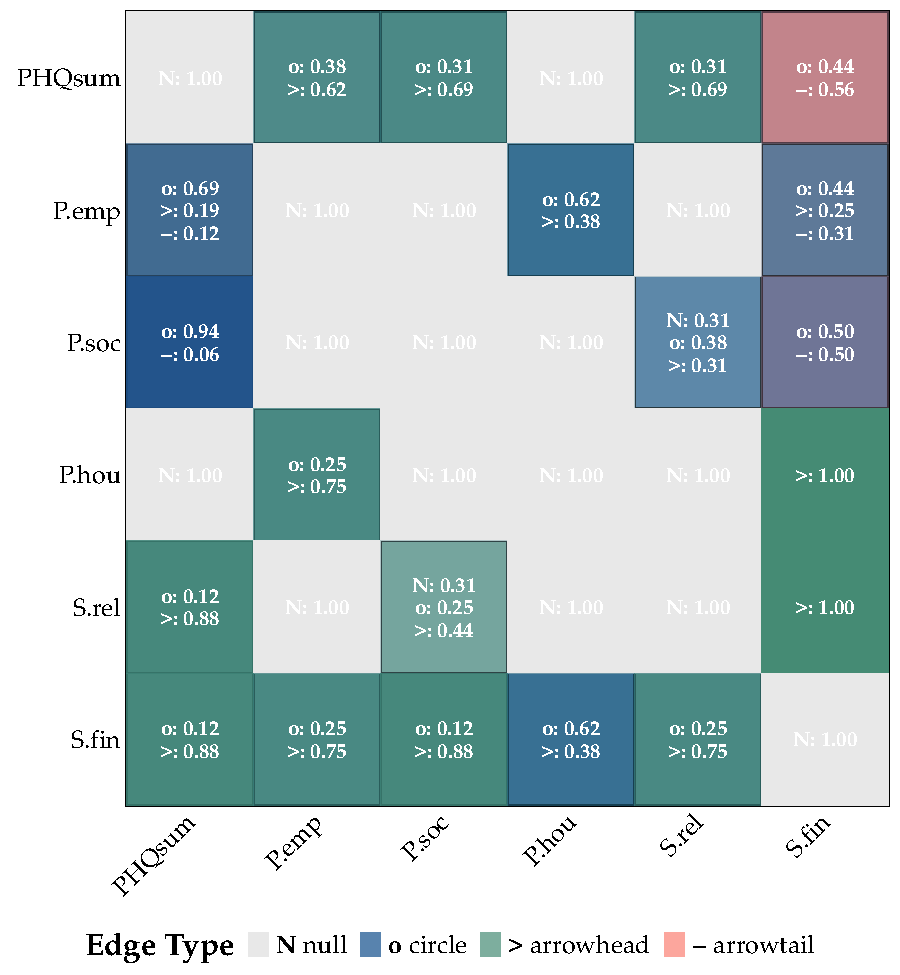
\includegraphics[width=1\textwidth,height=\textheight]{img/depsum_mat_fci.pdf}

}

\subcaption{\label{fig-sum-2}Proportion matrix}

\end{minipage}%

\caption{\label{fig-sum}\textcolor{BrickRed}{\textit{\textbf{Graph summaries of associations between precariousness factors and overall depression severity.}} In the FCI outputs, financial stress (\textit{S.fin}) shows the most \textcolor{BrickRed}{consistent adjacency} with depression severity (\textit{PHQsum}) across bootstrap resamples and specifications, whereas other precariousness domains show weaker or more variable connections.}
\textbf{(a)}
\textcolor{BrickRed}{Aggregated FCI summary graph showing the most frequent edge marks across bootstraps. The summary emphasizes the consistently recovered adjacency between \textit{S.fin} and \textit{PHQsum}, while other connections are more variable across specifications.}
Dashed edges indicate ties in the most frequent edge mark across the
specification grid, with a bold horizontal bar marking where the tie
occurs. \textbf{(b)} Proportion matrix (selection frequencies across
bootstrap resamples) summarizing edge marks across all bootstraps: each
matrix cell \([i, j]\) indicates how often a given edge from variable
\(i\) to variable \(j\) exhibited a particular edge mark (e.g.,
arrowhead, tail, or circle) adjacent to \(j\). Green indicates
arrowheads, coral tails, blue circle marks, and gray absence of an edge.
Colors are blended and shaded by frequency, with dominant symbols
appearing more opaque. For example, matrix{[}\(\mathit{S.fin}\),
\(\mathit{PHQsum}\){]} shows a green arrowhead and
matrix{[}\(\mathit{PHQsum}\), \(\mathit{S.fin}\){]} shows a coral tail,
\textcolor{BrickRed}{together indicating an edge mark pattern consistent with $\mathit{S.fin} \rightarrow \mathit{PHQsum}$ in the majority of bootstrapped graphs.}}

\end{figure}%

\subsubsection{Individual depression
symptom}\label{individual-depression-symptom}

Moving from the sum score representation to the disaggregated
symptom-level graph provides a more granular perspective on the causal
relationships between precariousness factors and depression symptoms.
Unlike the sum score graph, which aggregates all symptoms into a single
measure, the symptom-level graph in Figure~\ref{fig-sym} reveals the
heterogeneity in how specific symptoms (\emph{con} (concentration),
\emph{slp} (sleep), \emph{ene} (energy), \emph{app} (appetite),
\emph{mot} (motor), \emph{sui} (suicidal), \emph{anh} (anhedonia),
\emph{glt} (guilt), and \emph{dep} (depressed mood)) are influenced by,
and in turn influence, different forms of precariousness.

Figure~\ref{fig-sym-1} reveals a strong interdependence among symptoms
and suggests much presence of latent confounders, as indicated by
numerous bidirectional edges. In Figure~\ref{fig-sym-2}, the proportion
matrix indicates that arrowheads are the most frequently inferred edge
type. However, circle endpoints are particularly common for \emph{anh},
\emph{slp}, \emph{ene}, and \emph{sui}, reflecting uncertainty in the
causal direction among these symptoms. Notably, the only arrowtail
connection appears between \emph{dep} and \emph{anh}, suggesting that
anhedonia is a potential cause of depressed mood.

Looking at the symptom-precariousness connections, one of the key
patterns is that ties are most frequently found in the relationships
between individual symptoms and precariousness factors. This suggests
that these causal links may be less stable across different conditions.
Closer examination reveals that most ties arise due to discrepancies
between the Gaussian CI test and the RCoT test---with Gaussian CI
favoring arrowheads and RCoT more often predicting the absence of an
edge.

Despite these differences, some consistent patterns emerge across both
CI tests, particularly in the case of \emph{S.fin}, which appears to be
connected to nearly all other variables---though many of these
connections are marked by ties, reflecting uncertainty in
directionality. One exception is the stronger evidence suggesting that
\emph{S.fin} may cause changes in \emph{app}, while its relationships
with other symptoms, such as \emph{ene}, \emph{mot}, and \emph{dep},
remain ambiguous. Similarly, \emph{P.soc} exhibits numerous connections
with depressive symptoms, with most edges pointing toward \emph{P.soc}
rather than outward from it. This suggests that depressive symptoms,
particularly \emph{dep} and \emph{glt}, may contribute to worsening
social precariousness rather than the other way around. Additionally,
\emph{anh} also shows signs of a potential causal influence on
\emph{P.soc}, reinforcing the idea that social precariousness is more
often a consequence rather than a driver of depressive symptoms.

Other precariousness factors exhibit more uncertainty but still notable
relationships. \emph{S.rel} is connected to \emph{slp}, \emph{glt}, and
\emph{app}, though directionality remains unclear in many cases.
\emph{P.emp} also connects to symptoms like \emph{slp}, \emph{mot}, and
\emph{con}, but, like \emph{S.rel}, these relationships exhibit a 50/50
split in directionality, reflecting uncertainty in the inferred causal
paths. In line with the aggregated graph in Figure~\ref{fig-sum},
\emph{P.hou} does not appear to have any direct relationship with
depression symptoms but consistently shows associations with
\emph{P.emp} and \emph{S.fin}. The causal relationships among
precariousness factors remain largely unchanged from the aggregated
analysis, with \emph{S.fin} exhibiting the strongest tendency to
influence other precariousness factors.

Among depressive symptoms, \emph{dep}, \emph{glt}, and \emph{slp} appear
to be the most connected to precariousness factors, while \emph{P.soc}
has the most connections with symptoms, predominantly as a recipient
rather than a driver of influence. Within the symptom network,
\emph{slp}, \emph{sui}, and \emph{anh} emerge as causally influential
symptoms, as they exhibit more outgoing arrows compared to other
symptoms. On the other hand, \emph{con}, \emph{mot}, \emph{dep}, and
\emph{glt}, despite having high connectivity, predominantly receive
incoming arrows, indicating they are more likely effects rather than
causes. Considering both symptom-precariousness connections and
symptom-level dynamics, \emph{slp} emerges as a central symptom, given
its strong ties to precariousness factors and its influential role
within the symptom network. \emph{P.soc} appears to function as a bridge
between the depression and precariousness subsystems, as depressive
symptoms appear to feed back into social precariousness, reinforcing a
self-sustaining dynamic between depression and precarious conditions.

Finally, the results from CCI are largely consistent with those from
FCI, but with some key differences. CCI tends to favor arrowheads more
frequently, resulting in a greater number of bidirectional edges, which
suggests a higher involvement of latent confounders. Additionally, CCI
exhibits more tie situations, though, similar to FCI, most ties occur
between absence and arrowhead edges, reflecting the discrepancy between
the Gaussian CI test and RCoT---where the Gaussian test favors
arrowheads, while RCoT more often suggests the absence of an edge. For a
detailed visualization of the CCI-derived graph and proportion matrix,
see Figure~\ref{fig-sym-cci}.

\textcolor{BrickRed}{\textbf{Main takeaway.} At the symptom level, sleep disturbance (\textit{slp}) is highly connected, and multiple configurations are consistent with depressive symptoms feeding into social precariousness (\textit{P.soc}), but many symptom–precariousness directions are unstable across CI tests and specifications.}

\newgeometry{top=10mm, bottom=20mm, left=40mm, right=40mm}

\begin{figure}

\begin{minipage}{\linewidth}

\centering{

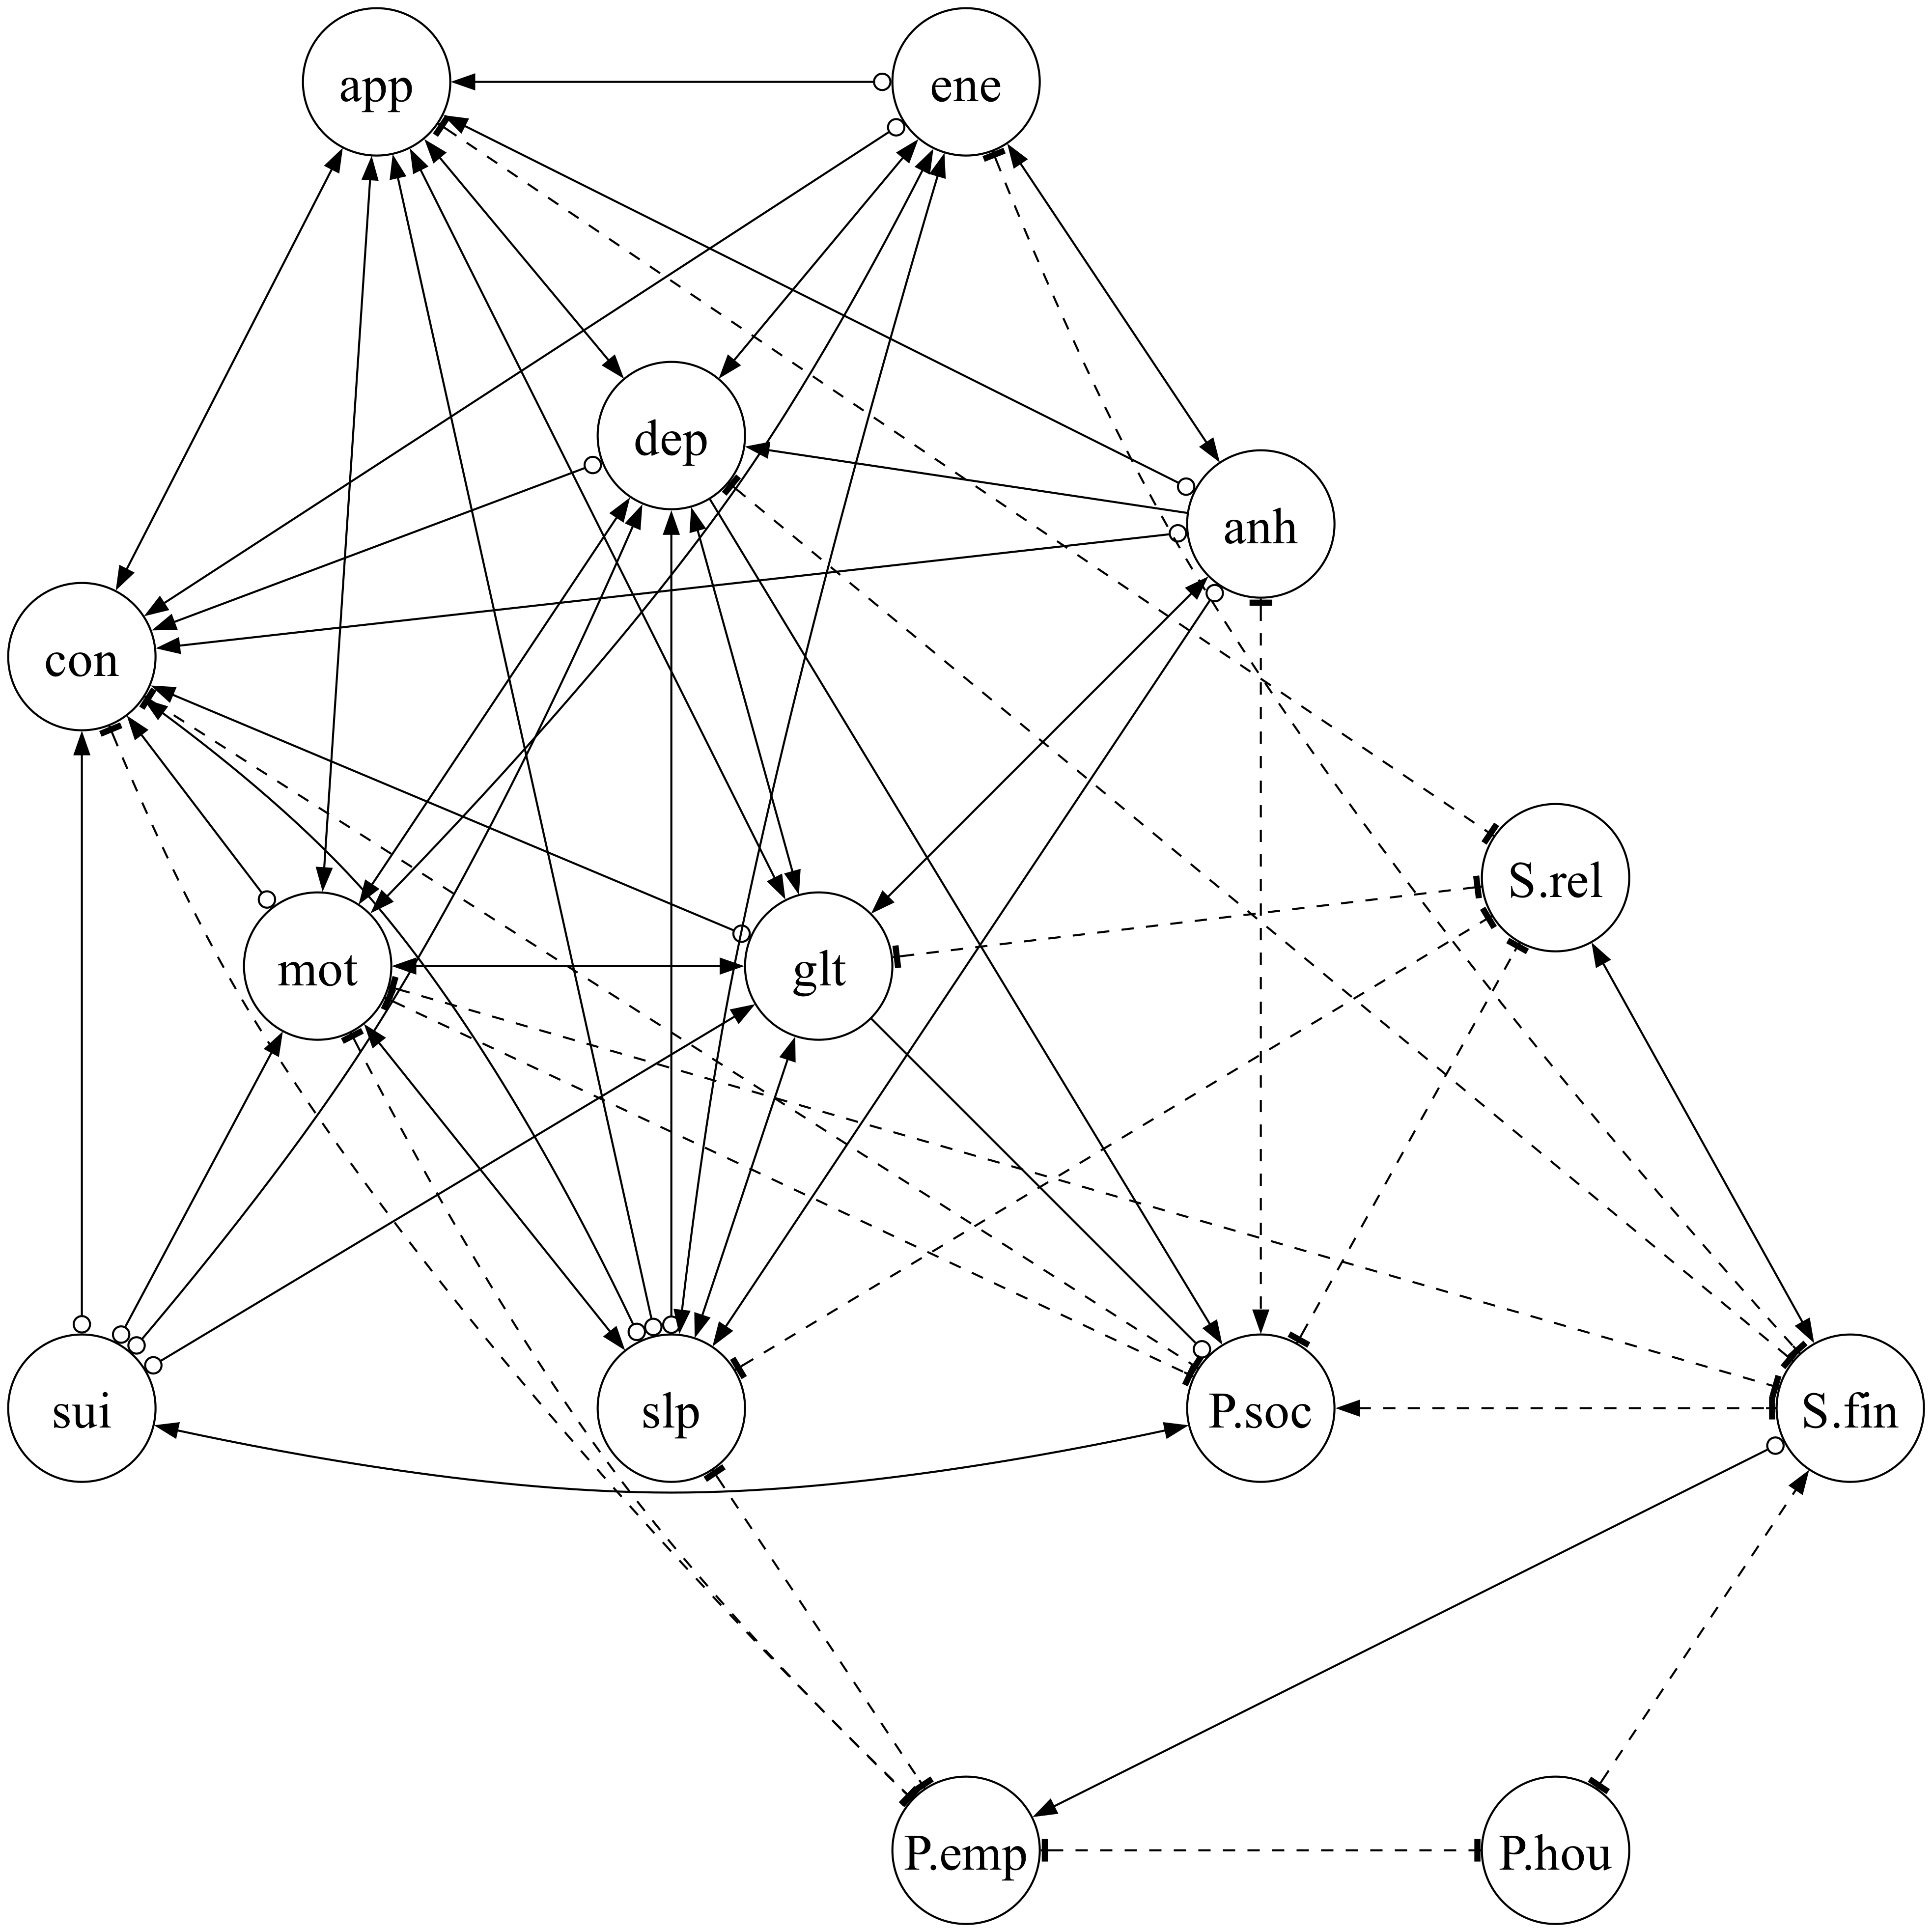
\includegraphics[width=0.6\textwidth,height=\textheight]{img/symptom_graph_FCI.png}

}

\subcaption{\label{fig-sym-1}FCI PAG}

\end{minipage}%
\newline
\begin{minipage}{\linewidth}

\centering{

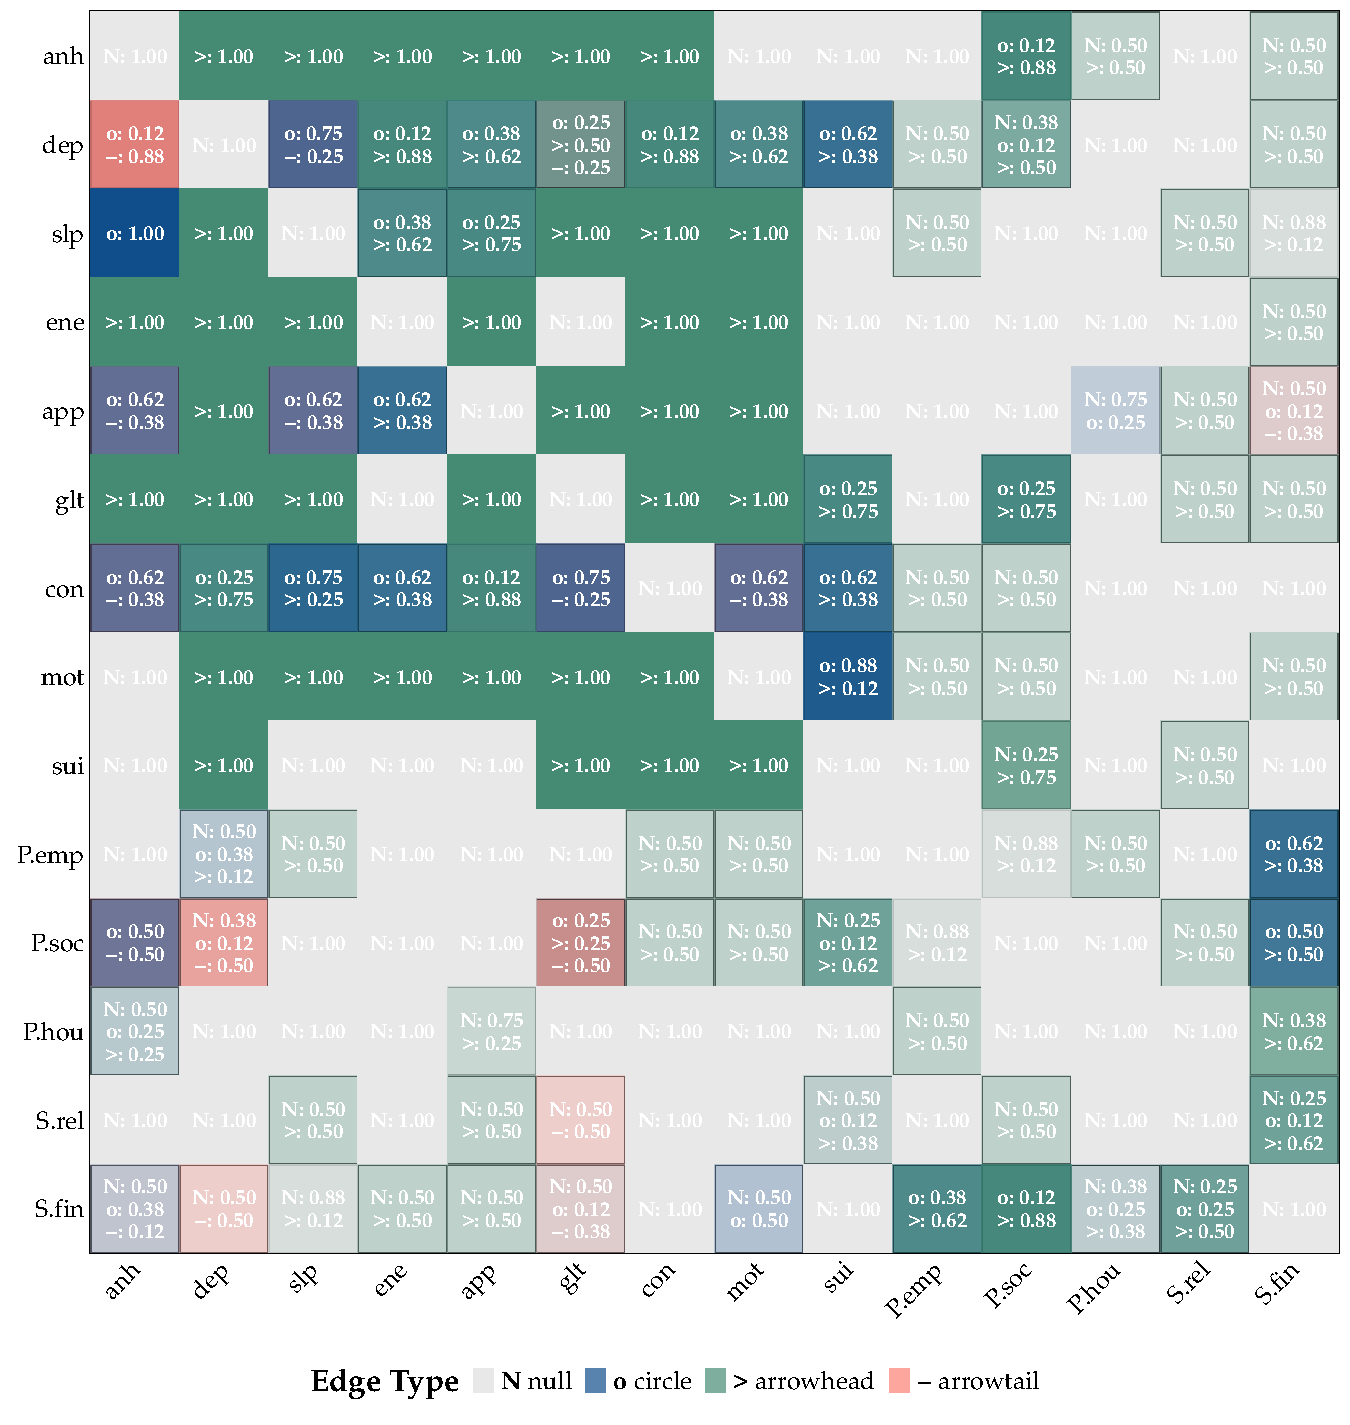
\includegraphics[width=0.6\textwidth,height=\textheight]{img/symptom_mat_fci.pdf}

}

\subcaption{\label{fig-sym-2}Proportion matrix}

\end{minipage}%

\caption{\label{fig-sym}\textbf{\emph{Causal pathways linking individual
depressive symptoms and precariousness factors.}} \textbf{(a)}
Aggregated FCI graph summarizing the most frequent edge types across
bootstraps. The pattern suggests that depressed mood (\emph{dep}), guilt
(\emph{glt}), and anhedonia (\emph{anh}) often direct influence into
social precariousness (\emph{P.soc}), indicating that \emph{P.soc} is
more likely a consequence of core depressive symptoms than their cause.
Sleep disturbance (\emph{slp}) emerges as central within the broader
network, with strong ties to several precariousness factors. Housing
precariousness (\emph{P.hou}) remains largely disconnected from
symptoms, instead linking to employment and financial stress.
\textbf{(b)} Proportion matrix showing edge-type frequencies across
bootstraps. Arrowheads are the most frequent endpoint overall, while
circle marks---reflecting uncertainty or latent confounding---are
particularly common for \emph{slp}, \emph{anh}, \emph{ene}, and
\emph{sui}.}

\end{figure}%

\restoregeometry

\subsubsection{Precariousness as sum
score}\label{precariousness-as-sum-score}

Lastly, we examine the relationships between individual symptoms and
overall precariousness, an aggregated measure represented by the sum of
five precariousness factors. This analysis provides a complementary
perspective, capturing broader patterns that may not be evident in the
disaggregated symptom-precariousness analysis. By aggregating
precariousness factors into a single score, this approach may capture
distributed relationships across different precariousness factors that
were previously overlooked in the disaggregated analysis.

Unlike the disaggregated graph in Figure~\ref{fig-sym}, the aggregated
symptom-precariousness graph (Figure~\ref{fig-presum-1}) shows greater
certainty in causal directions, with ties occurring only in edges
involving the overall precariousness factor. This is even more evident
in the proportion matrix (Figure~\ref{fig-presum-2}), where
symptom-to-symptom interactions almost fully converge to a single edge
type. Additionally, all symptom interactions are connected either
through bidirectional edges or a combination of an arrowhead and a
circle, suggesting a strong presence of latent confounders.

Examining the symptom-precariousness connections, we observe a stronger
overall trend of depressive symptoms influencing precariousness, rather
than the other way around. Specifically, \emph{anh}, \emph{dep}, and
\emph{slp} frequently emerge as sources of influence on precariousness,
whereas \emph{app}, \emph{glt}, and \emph{mot} exhibit more uncertainty
in directionality, often resulting in circle endpoints. This pattern
suggests that when precariousness factors are aggregated, the dominant
causal flow is from depressive symptoms to precariousness, rather than
precariousness driving depression. Particularly, \emph{dep} emerges as
the strongest predictor of precariousness, exhibiting the highest
proportion of arrowtails, consistent with findings from the
disaggregated analysis.

Comparing this with the CCI-derived graph (Figure~\ref{fig-presum-cci}),
several key differences stand out. The CCI results reveal that most
symptoms are interconnected through bidirectional edges, suggesting a
strong presence of latent confounders. However, \emph{dep} appears to be
a distinct exception, as it is predominantly caused by nearly all other
symptoms, with one exception \emph{sui}, which does not contribute to
\emph{dep}. Similarly, \emph{con} is influenced by multiple symptoms,
albeit with weaker support compared to \emph{dep}. Most interestingly,
the CCI results highlight a distinct feedback loop between \emph{dep}
and overall precariousness, represented by a tail-tail edge
(\textemdash ). This suggests a possible reinforcing cycle between
depression and overall precariousness, where depression not only arises
from precarious conditions but also contributes to their persistence,
creating a self-sustaining dynamic.

\textcolor{BrickRed}{Across multiple levels of analysis, our results show consistent connections between precariousness and depression, with the most stable adjacency linking financial stress (\textit{S.fin}) to depressive outcomes. Across many specifications, edge marks are more often compatible with financial stress preceding depression, although directionality remains partly indeterminate and varies with modeling choices. Other precariousness dimensions, especially social precariousness, more often appear downstream of depressive symptoms or remain unresolved. At the symptom level, \textit{dep} and \textit{slp} stand out for their connectivity to precariousness factors, with several configurations consistent with feedback between these factors involving social precariousness. On this basis, we use a simplified three-node simulation model of depression, financial stress, and social precarity to examine how alternative plausible feedback strengths, which cannot be identified from cross-sectional data, shape trajectories under stress-reducing scenarios.}

\textcolor{BrickRed}{\textbf{Main takeaway.} When precariousness is aggregated, symptom-to-precariousness orientations appear more consistent than in the fully disaggregated setting, and some configurations are compatible with feedback between depression and overall precariousness, though directionality remains method-dependent.}

\newgeometry{top=10mm, bottom=20mm, left=40mm, right=40mm}

\begin{figure}

\begin{minipage}{\linewidth}

\centering{

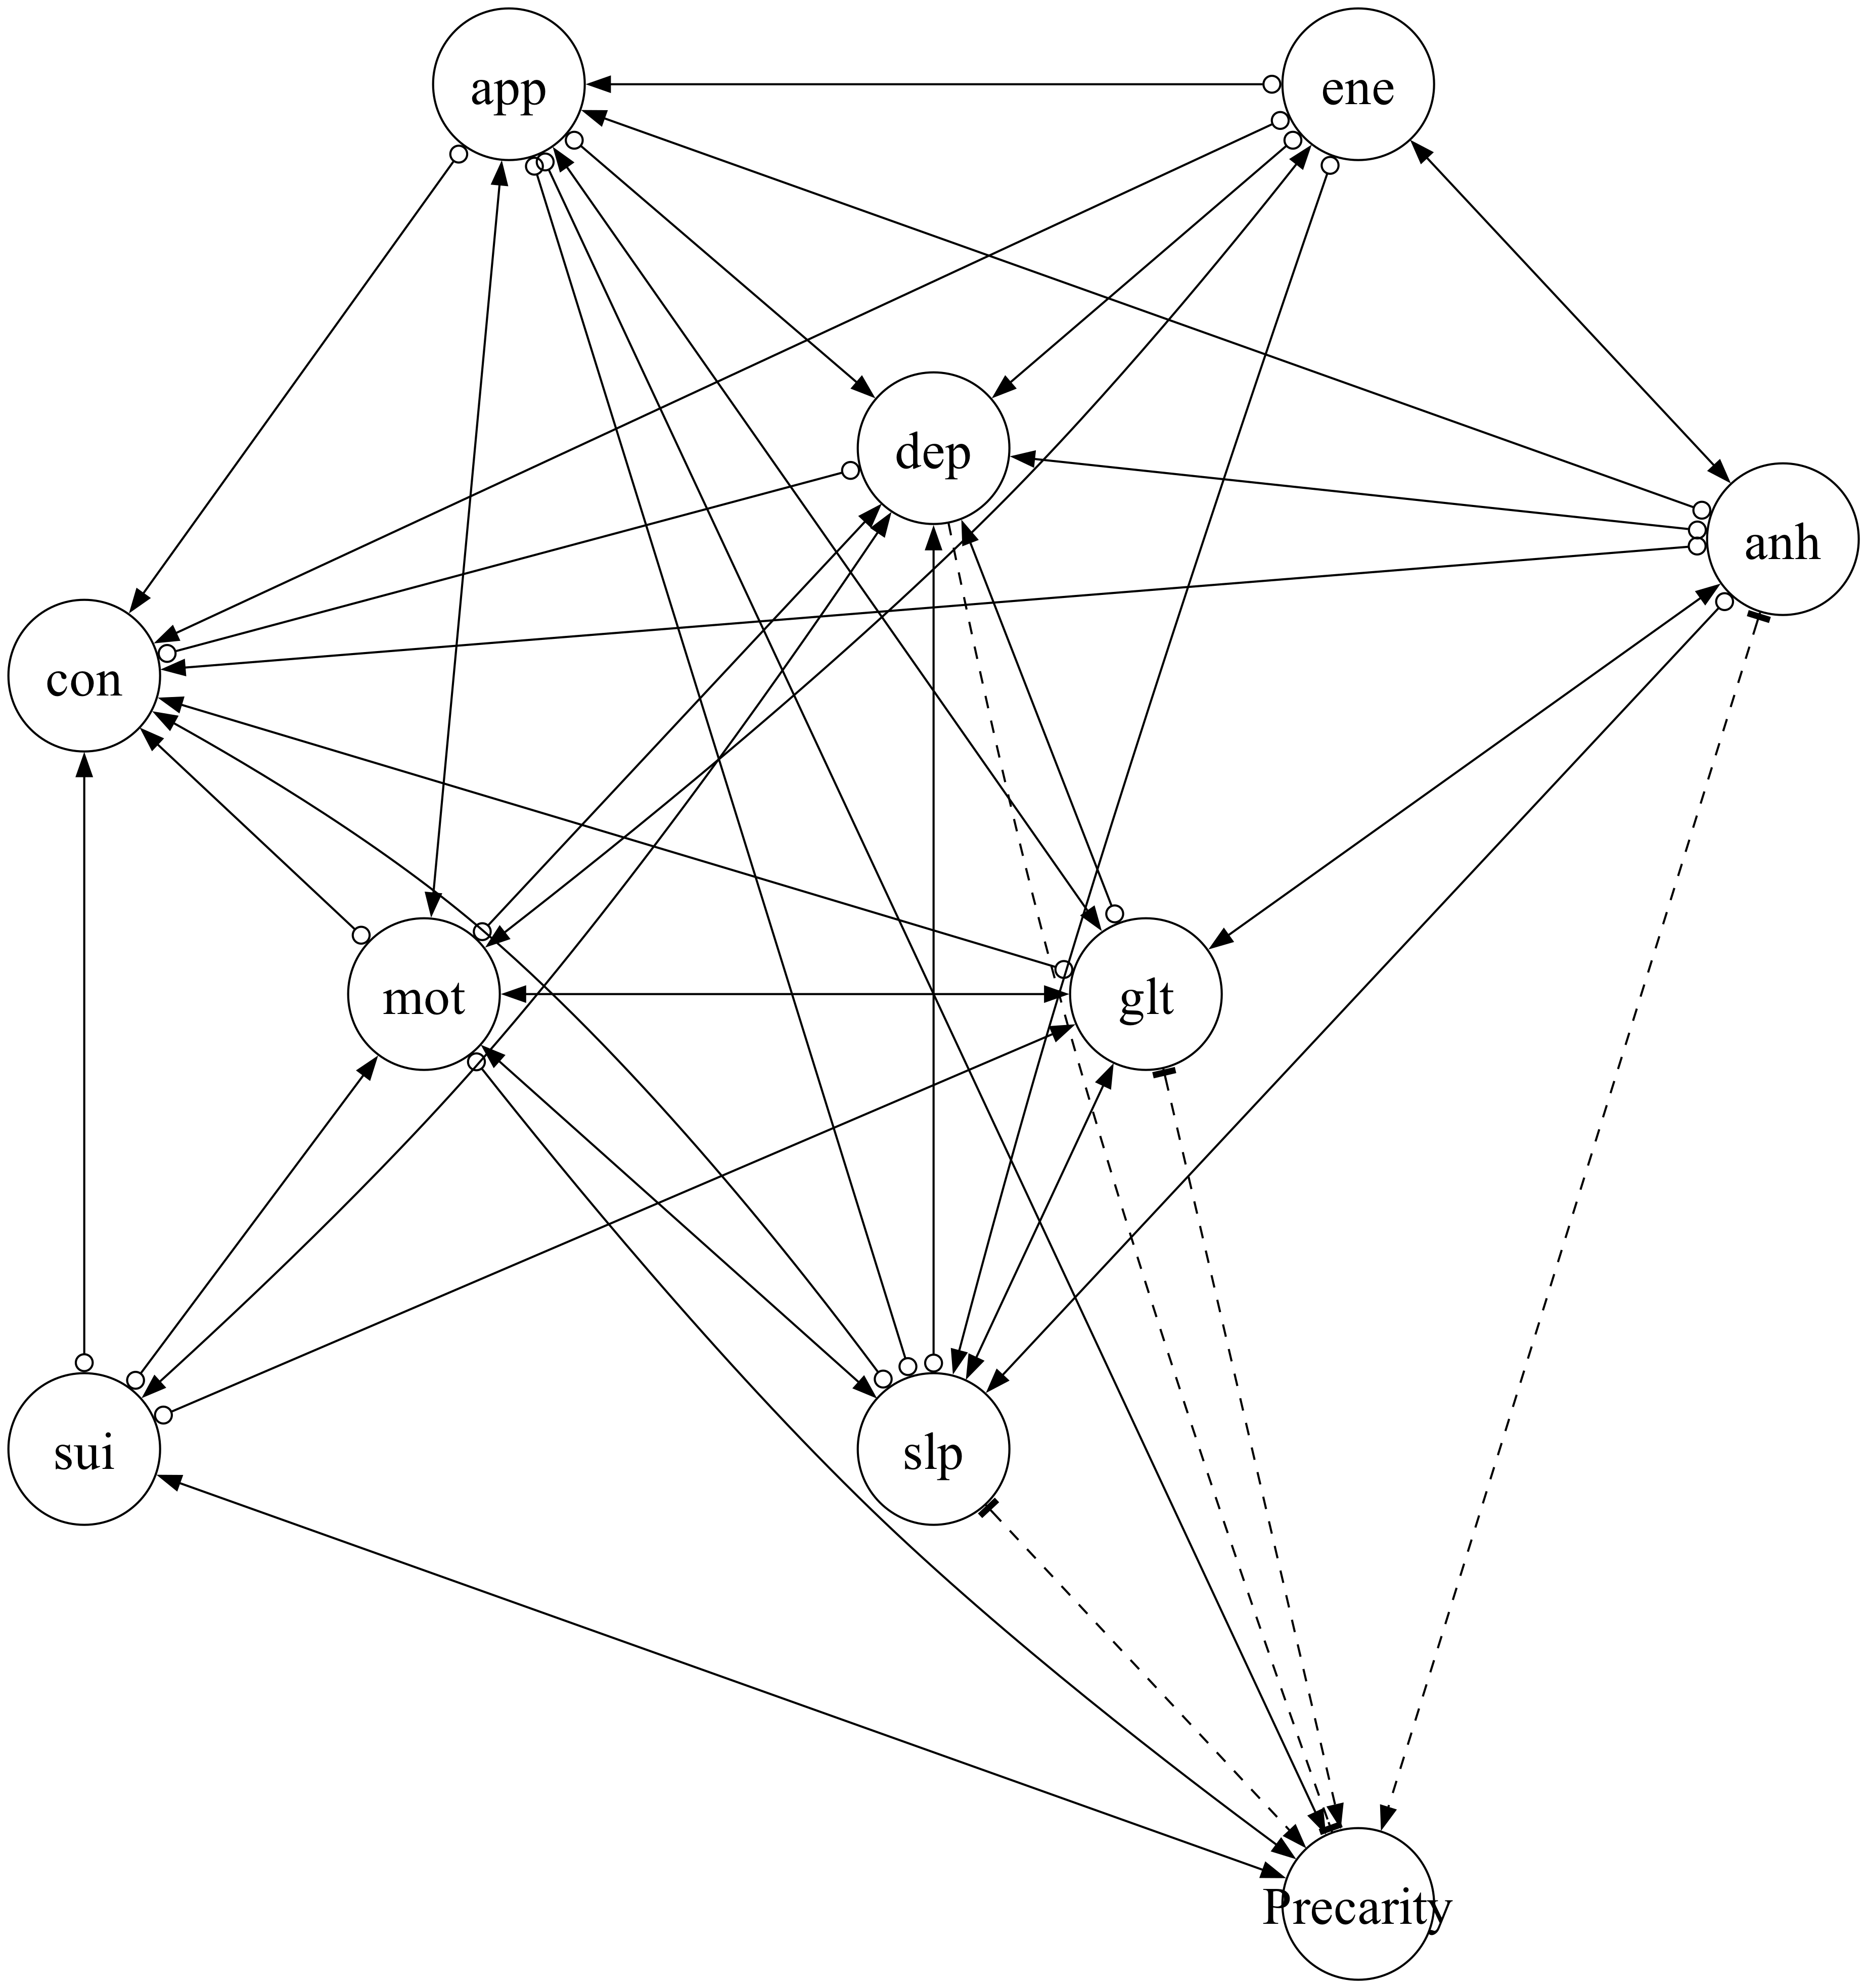
\includegraphics[width=0.6\textwidth,height=\textheight]{img/presum_graph_FCI.png}

}

\subcaption{\label{fig-presum-1}FCI PAG}

\end{minipage}%
\newline
\begin{minipage}{\linewidth}

\centering{

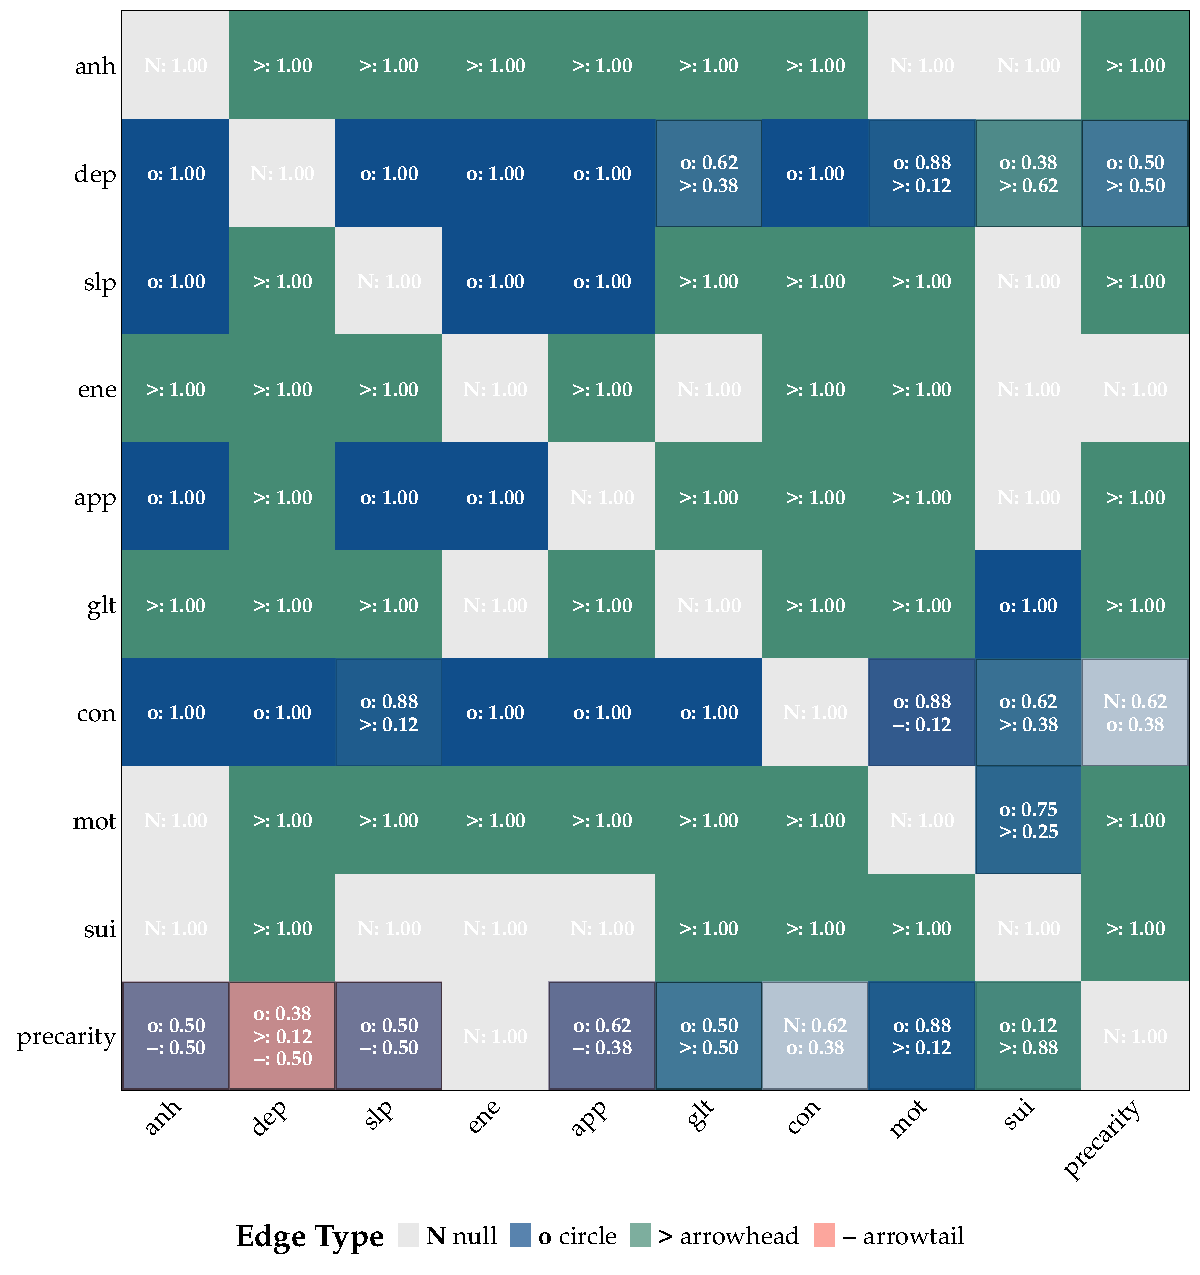
\includegraphics[width=0.6\textwidth,height=\textheight]{img/presum_mat_fci.pdf}

}

\subcaption{\label{fig-presum-2}Proportion matrix}

\end{minipage}%

\caption{\label{fig-presum}\textbf{\emph{Causal pathways between overall
precariousness and individual depressive symptoms.}} \textbf{(a)}
Aggregated FCI graph summarizing the most frequent edge types across
bootstraps. The edge pattern indicates that depressive
symptoms---particularly anhedonia (\emph{anh}), depressed mood
(\emph{dep}), and sleep disturbance (\emph{slp})---more often direct
influence into overall precariousness, rather than the reverse. By
contrast, symptoms such as appetite (\emph{app}), guilt (\emph{glt}),
and motor disturbance (\emph{mot}) show greater uncertainty in
directionality. \textbf{(b)} Proportion matrix showing edge-type
frequencies across bootstraps. Symptom-to-symptom connections converge
strongly on single edge types, with most interactions either
bidirectional or split between arrowhead and circle marks, consistent
with the presence of latent confounders.}

\end{figure}%

\restoregeometry

\subsection{Simulating the Dynamics Between Precariousness and
Depression Under
Intervention}\label{simulating-the-dynamics-between-precariousness-and-depression-under-intervention}

To assess how internal structure influences the system's responsiveness
to external support, we simulated a set of linear models consistent with
the observed data. The data constrain the strength of connections from
financial stress to both depression and precariousness, as well as the
total strength of feedback between these two domains. However, within
these bounds, multiple feedback configurations are compatible with the
data, differing in the dominant direction of influence. We characterize
these alternatives by the strength of the pathway from precariousness to
depression (\(\alpha_{DP}\); see trade-off in
Figure~\ref{fig-tradeoff}). For each model, we generate a virtual
population of 1,000 individuals, with baseline financial stress sampled
from the HELIUS data. We then simulate an external intervention that
reduces each individual's financial stress (\(S\)) proportionally toward
the minimum observed value in the dataset. While individuals begin with
different baseline stress levels, the intervention applies a shared
proportional reduction across the population. This intervention defines
the external input, while variation in \(\alpha_{DP}\) reflects
different assumptions about internal feedback from precariousness to
depression. We examine system behavior in two complementary ways: (1) by
analyzing average levels of depression and precariousness at selected
time points following intervention onset, and (2) by simulating full
temporal trajectories under sustained intervention followed by recovery,
using two representative cases at the extremes of the \(\alpha_{DP}\)
range.

Figure~\ref{fig-intervention} summarizes how variation in
\(\alpha_{DP}\) shapes system-level responses to external support. In
Panel A, during the early phase of intervention, depression and
precariousness exhibit contrasting patterns. Depression declines more
rapidly in scenarios with lower \(\alpha_{DP}\), where its dynamics are
driven more directly by the external stressor \(S\). As \(\alpha_{DP}\)
increases, \(D\) becomes more dependent on precariousness (\(P\)), which
itself adjusts more slowly---delaying the depressive response.
Precariousness, by contrast, shows slightly faster early reductions in
scenarios with higher \(\alpha_{DP}\). This reflects a shift in
influence: as \(\alpha_{DP}\) increases, \(P\) becomes more directly
responsive to \(S\) (via increasing \(\alpha_{PS}\)) and less influenced
by \(D\), allowing it to adjust more promptly to changes in the
stressor.

Despite these short-term differences, all scenarios ultimately converge
to similar steady-state levels under sustained intervention. AS the
systm approaches convergence, some variation remains, particularly in
\(P\), where gradients between models are still visible. This
convergence highlights that the key distinctions lie not in whether
intervention is effective, but in how quickly and through which pathways
change unfolds.

Panel B shows full time trajectories for two representative cases: one
with minimal internal feedback (\(\alpha_{DP} = 0\)) and one at the
upper admissible limit (\(\alpha_{DP} = 0.65\)). In both, there is a
temporary intervention period. When \(\alpha_{DP} = 0\), depression
responds rapidly to the reduction in stress and rebounds shortly after
support is withdrawn. In contrast, when \(\alpha_{DP}\) is high, \(D\)
responds more gradually and recovers more slowly---reflecting its
increased dependence on the slower-changing \(P\). Precariousness
declines in both scenarios during intervention and returns to baseline
afterward, but with a slightly sharper drop in the higher
\(\alpha_{DP}\) condition. This occurs because \(P\) becomes more
directly responsive to \(S\), as consistency with the data requires
\(\alpha_{PS}\) to increase with \(\alpha_{DP}\) (see
Figure~\ref{fig-tradeoff}). These parameter shifts reflect trade-offs
needed to preserve the empirical covariances, with further details
provided in Appendix Section~\ref{sec-analcalibration}.

These asymmetries further highlight how internal structure---not just
external inputs---shapes the system's trajectory. Specifically, changes
in coupling parameters reconfigure how stress reduction propagates
through the system, altering the speed and pathway of response even when
long-run outcomes remain unchanged.

\newgeometry{top=15mm, bottom=20mm, left=40mm, right=40mm}

\begin{figure}

\centering{

\includegraphics[width=0.8\textwidth,height=\textheight]{img/intervention_linear.pdf}

}

\caption{\label{fig-intervention}\textbf{\emph{System response to
external intervention across variations in internal structure.}}
\textbf{(A)} \emph{Mean levels of depression (\(D\)) and precariousness
(\(P\)) at key time points.} At time steps 100, 300, and 500, we compare
models that differ in the coupling coefficient \(\alpha_{DP}\), which
represents the strength of depression's influence on precariousness in
the dynamical model. The x‑axis shows intervention strength, defined as
the proportional reduction of financial stress (\(S\)) relative to its
baseline (with higher values indicating more external financial
support). Each line corresponds to a different model, color-coded from
weak (purple) to strong (yellow) coupling. Models with weaker coupling
exhibit faster early reductions in \(D\), while stronger coupling shifts
the response toward \(P\), producing more immediate declines in
precariousness. \textbf{(B)} \emph{Full temporal trajectories under weak
coupling versus strong coupling.} Time series illustrate intervention
onset (step 300) and withdrawal (step 1500) for two representative
cases: one with no coupling (\(\alpha_{DP} = 0\)) and one with strong
coupling (\(\alpha_{DP} = 0.65\)). Depression responds more gradually
and persistently under strong coupling, whereas precariousness adjusts
more quickly.}

\end{figure}%

\restoregeometry

\section{Discussion}\label{discussion}

This study combined constraint-based causal discovery and dynamical
modeling to investigate how depression and socioeconomic precariousness
interact and how their internal structure modulates responsiveness to
intervention. Consistent with prior work linking financial strain to
psychological distress (Ezzy, 1993; Lund et al., 2010),
\textcolor{BrickRed}{the most consistent finding from the causal discovery stage is the stable adjacency between recent financial stressors (\textit{S.fin}) and depression (PHQsum / symptoms) across bootstrap resamples and across our prespecified specification grid. Beyond this adjacency, directional information is substantially less stable: endpoint marks vary across algorithms and CI tests, and many orientations remain unresolved.}
\textcolor{BrickRed}{
Across bootstrap resamples and across our prespecified specification grid, the most consistent finding from the causal discovery stage is the stable adjacency between recent financial stressors (\textit{S.fin}) and depression (PHQsum / symptoms). Beyond this adjacency, directional information is substantially less stable: endpoint marks vary across algorithms and CI tests, and many orientations remain unresolved. We therefore emphasize patterns that replicate across methods and interpret orientation marks conservatively, as equivalence-class (ancestral-constraint) information rather than identified causal effects. In particular, any directional tendency involving \textit{S.fin} and depression is treated as a data-compatible hypothesis, while the stable \textit{S.fin}--depression connection motivates the broader hypothesis that economic stressors may contribute to cycles of psychosocial risk.}
\textcolor{BrickRed}{
With this framing, the causal discovery stage serves to identify which structural motifs are consistently supported (and where direction collapses into indeterminacy), and the simulation stage then explores how different plausible feedback regimes—compatible with the observed moments and those stable motifs—translate into different intervention trajectories.}

\textcolor{BrickRed}{Several estimated configurations are compatible with mutually reinforcing dynamics, but the present analyses do not identify a single reinforcement pathway. Instead, they delineate the stable motifs and key uncertainties, motivating follow-up work with stronger identifying information to clarify reinforcement mechanisms and quantify policy-relevant effects.}
At the symptom level, our analysis aligns with established theories of
psychopathology and provides a more fine-grained map of potential causal
relationships, generating concrete, testable hypotheses. It points to
possible limitations of prevailing models, as some observed
symptom--symptom links may be shaped by shared confounders rather than
direct causal influence. This suggests that, in some contexts, broader
mechanisms or clusters of symptoms may provide more effective units of
analysis and intervention than individual symptoms alone.
\textcolor{BrickRed}{Within this framework, sleep disturbance emerged as a candidate initiating symptom, with directed connections to both symptom-level and precariousness variables. This aligns with longitudinal findings that identify sleep disruption as an early signal for depressive episodes and social withdrawal}
(Alvaro et al., 2013; Zawadzki et al., 2013). Depressed mood, another
core symptom, occupied a central position in the network.
\textcolor{BrickRed}{It was influenced by symptoms such as anhedonia and guilt, and it also showed directed links to social precariousness. This pattern is consistent with pathways in which internal psychological states contribute to external vulnerability. The CCI algorithm further returned a candidate feedback relation between depressed mood and overall precariousness, which is in line with social drift theories in depression, where declining mental health can lead to social exclusion, job instability, and housing insecurity, reinforcing depressive cycles}
(Boschloo et al., 2015; Compton \& Shim, 2015).

In contrast, social precariousness itself appeared more often as an
effect than a cause, receiving arrows from symptoms like depressed mood
and guilt but rarely sending them. This asymmetry supports prior
observations that indicators of social vulnerability often reflect
downstream consequences of poor mental health, though the relationships
are likely bidirectional over time (Lund et al., 2010). Although our
findings are based on Amsterdam-specific data, they align with research
in other high-income urban settings, where structural inequalities such
as poverty, unemployment, and housing insecurity consistently predict
poor psychological outcomes (Fryers et al., 2003; Weich \& Lewis, 1998).
\textcolor{BrickRed}{While local contexts may alter specific pathways, these parallels suggest that similar mechanisms could operate elsewhere; replication in other populations is needed to assess generalizability.}

\textcolor{BrickRed}{These results suggest several implications for intervention design. Symptoms such as sleep disturbance, which show broad connectivity to both symptom and precariousness variables, may be useful targets for prevention in some settings, potentially reducing escalation into more persistent depressive states or worsening social vulnerability. In addition, symptoms that appear embedded in candidate feedback relations linking psychological and social domains, such as depressed mood, may offer leverage points for disrupting mutually reinforcing cycles.}
Importantly, interventions targeting such cycles may have ripple effects
across domains. For instance, evidence suggests that treating core
depressive symptoms can improve social functioning, employment
engagement, and housing stability, particularly when combined with
social or financial supports (Lund et al., 2018; McDaid et al., 2019).
These dual benefits underscore the value of integrated, cross-domain
strategies that simultaneously address internal symptoms and external
stressors, and show promise of the external validity of our analysis.

\textcolor{BrickRed}{Our results also highlight why single-point interventions may fail to produce lasting change. The estimated graphs include several reciprocal links spanning psychological symptoms and structural risk factors, which could re-amplify vulnerability after temporary relief.}
Supporting this, recent simulation work shows that feedback loops, even
when modest in strength, can substantially diminish the long-term impact
of isolated interventions unless multiple reinforcing links are
simultaneously disrupted (Park, Li, et al., 2025). Our own simulations
support this view: while all models converged to similar long-term
outcomes under sustained support,
\textcolor{BrickRed}{differences in internal structure, particularly the assumed direction and strength of coupling between precariousness and depression, produced systematic variation in how quickly and through which pathways systems responded to intervention.}
Stronger coupling from precariousness to depression slowed recovery and
prolonged depression, showing that internal architecture can be as
important as external input. This supports growing calls for
systems-oriented mental health perspectives (Borsboom, 2017). Rather
than assuming uniform responses, more durable outcomes may require (1)
targeting early-acting symptoms, (2) sustaining support where recovery
is slow, and (3) combining structural and psychological interventions.
Tailoring strategies to match the system's architecture can improve
effectiveness, particularly in populations with layered vulnerabilities.
\textcolor{BrickRed}{In this context, clarifying plausible causal structure is important for designing more effective and equitable interventions.}

\textcolor{BrickRed}{Because the intervention variables are measured proxies and the data are cross-sectional, the simulations should be interpreted as scenario analyses of proxy shifts.}
\textcolor{BrickRed}{We interpret the causal discovery results as equivalence-class constraints and stability summaries, and we treat them as hypothesis-generating inputs that motivate future longitudinal or quasi-experimental evaluation.}
\textcolor{BrickRed}{Two limitations are particularly relevant for interpreting the estimated graph summaries. First, selection bias is a plausible concern in this setting. HELIUS has a modest participation rate, and our analyses condition on completion of the questionnaire items used in the current study. Conditioning on participation and complete-case inclusion can induce associations among measured variables, including collider-type dependencies, which could appear as edges in graph learning. Because the discovery procedures used here do not explicitly model selection, we cannot separate selection-induced associations from associations that would persist under representative sampling without additional information. Methodological work on causal discovery under selection mechanisms is currently active. Recent SCM-based developments formalize selection as conditioning on a selection variable and characterize when such conditioning induces spurious associations that need not reflect target-population relations}
(Chen et al., 2024).
\textcolor{BrickRed}{In light of these theoretical developments, future work could incorporate explicit models of participation and missingness, weighting strategies, or auxiliary design information, with the goal of evaluating how robust the recovered adjacency patterns are to plausible selection mechanisms.}
\textcolor{BrickRed}{Second, even in the absence of selection bias, edge orientations can remain ambiguous in cross-sectional data with measurement error and finite samples. In our results, many directions vary across algorithms, conditional independence tests, and resampling, particularly for symptom-level relations, which likely reflects limited statistical signals in high-dimensional settings. We therefore avoid treating orientation patterns as identified directionality and instead report them as stability summaries. 
Future work could combine theory-guided subgraph restriction with longitudinal or quasi-experimental data, and could assess orientation stability under a wider range of tuning choices or alternative conditional-independence tests, to determine which directional constraints persist under designs with stronger identifying information.}
\textcolor{BrickRed}{A further limitation is that we do not examine whether the recovered motifs differ across ethnicity, gender, age, or SES, despite HELIUS being a multi-ethnic cohort. This question matters because both participation and item nonresponse may vary across subgroups, so subgroup-specific analyses would be more sensitive to selection and measurement differences, making it difficult to separate genuine structural heterogeneity from artifacts of differential missingness, measurement non-invariance, or reduced statistical information per group. We view subgroup heterogeneity as an important direction for future work, ideally paired with explicit checks of measurement comparability and robustness to plausible selection mechanisms.}

Moreover, some relations showed sensitivity to the choice of conditional
independence (CI) test. The Gaussian CI test, which assumes linearity
and Gaussian noise, often produced denser graphs, plausibly because
partial-correlation tests can be more permissive for weak linear
associations in large samples. In contrast, RCoT avoids strict Gaussian
assumptions and can capture nonlinear dependencies, but it relies on
kernel-based approximations (via random Fourier features) and, in
practice, performance can vary with variable type and distributional
properties. In particular, kernels commonly used in this setting (e.g.,
RBF kernels) are optimized for smooth relationships among continuous
variables and may behave differently for ordinal or mixed-type measures,
which is relevant for HELIUS (Howlett, 2001).
\textcolor{BrickRed}{Two complementary directions could help address this in future work. First, CI testing could be adapted to better handle mixed data structures, for example by employing hybrid kernels or test procedures that explicitly combine continuous and discrete similarity measures, and by systematically evaluating sensitivity across a wider range of CI tests and tuning choices. Second, applying additional discovery families may be informative under alternative identifying assumptions. 
For example, functional-model identification approaches that exploit non-Gaussianity or additive-noise assumptions—such as LiNGAM}
(Shimizu et al., 2006) \textcolor{BrickRed}{and additive-noise models}
(Hoyer et al.,
2008)\textcolor{BrickRed}{—can be useful under acyclicity and stronger functional-form restrictions, although these assumptions do not align with our target setting and we therefore treat them as a complementary extension rather than a primary approach here. Relatedly, invariance-based approaches such as Invariant Causal Prediction (ICP;}
Peters et al.
(2016)\textcolor{BrickRed}{) aim to identify causal drivers of a response by leveraging stability of the conditional distribution across multiple environments (e.g., interventions, sites, policy contexts, or time periods). This is appealing for "what drives depression?" questions, but it requires meaningful environment structure that is not available for our central variables in the baseline data from the HELIUS cohort, and standard ICP targets acyclic parent sets; extensions exist but still require environments. We therefore view ICP as a promising direction for future work once data with explicit environment variation become available, for example through quasi-experimental designs, pre/post-policy contrasts, or longitudinal settings that generate meaningful differences across waves.}

Although the CCI algorithm is explicitly designed to detect cycles,
aside from the connection between precarity and depression in the
aggregate precarity setting, we found little clear evidence of feedback:
most candidate loops appeared only as bidirectional edges, which may
reflect latent confounding or statistical imprecision. This could point
to either an absence of strong feedback at the symptom and the
precariousness factor levels or limitations in the sensitivity of
full-graph discovery approaches applied to densely interconnected
variables. More focused strategies, such as local structure tests or
theory-guided subgraph modeling, may help resolve these ambiguities.
Moreover, our analyses relied solely on observational data from the
Amsterdam population. Some structural uncertainties, particularly those
involving latent confounding or bidirectional influence, may ultimately
require interventional or semi-interventional designs. Extensions such
as LLC (Hyttinen et al., 2012), NODAGS-Flow (Sethuraman et al., 2023),
or Bicycle (Rohbeck et al., 2024), which integrate observational and
interventional data, could be especially valuable where such data are
available.

\textcolor{BrickRed}{Because the simulation uses a linear Ornstein–Uhlenbeck specification calibrated to match the same empirical second-order moments, some qualitative response patterns, such as differences in adjustment speed as coupling varies, are expected properties of linear relaxation dynamics. We therefore do not interpret the OU behavior itself as a novel dynamical finding. Rather, we use it as a transparent baseline to carry forward the most stable motif identified in the discovery stage and to treat feedback strength as a sensitivity/uncertainty dimension, rather than fixing a single value that is not well constrained in the present setting.}

Finally, the structure of our dynamical model introduces important
limitations. The model focused on a restricted set of variables
(depression, social precariousness, and financial stress). This design
was intentionally simplified to isolate core mechanisms of interest, but
it necessarily omits other relevant domains of precariousness,
additional stressors, and potential unintended consequences of
intervention. In addition, while the linear formulation offered
analytical tractability and transparent calibration, it likely
oversimplifies the true dynamics of depression and socioeconomic
precariousness.
\textcolor{BrickRed}{A growing body of evidence suggests that psychosocial systems are fundamentally nonlinear. Empirical and theoretical work points to phenomena such as threshold effects, where improvements only occur after a tipping point is crossed}
(Leemput et al., 2014; Park, Waldorp, et al., 2025);
\textcolor{BrickRed}{saturation, where the impact of support diminishes as basic needs are met}
(Cramer et al., 2010);
\textcolor{BrickRed}{and path dependence, where past adversity shapes sensitivity to future stressors}
(Wichers et al., 2016).
\textcolor{BrickRed}{These behaviors are not well captured by linear dynamics, yet they may be essential for understanding why some individuals remain trapped in high-risk states while others recover more easily. Future modeling efforts should therefore incorporate mechanisms such as saturating input-response functions (e.g., sigmoidal form) and state-dependent feedback where coupling strength varies by system state. Such nonlinear terms would allow the model to capture threshold-type deterioration (feedback becoming disproportionately strong beyond a critical depression level) as well as recovery nonlinearities, where improvements in precariousness translate into delayed or amplified reductions in depression only after crossing a recovery threshold. Incorporating such features would allow models to capture not just average effects but also the critical conditions under which meaningful change becomes possible, clarifying whether some subgroups require forceful, threshold-crossing interventions, while others may benefit from sustained, moderate support.}

As public health research has long shown, social and psychological
systems do not always respond passively to external inputs; internal
constraints can limit the impact of even well-intentioned policies
(Savigny \& Adam, 2009; Wagenaar \& Burris, 2013).
\textcolor{BrickRed}{By combining causal discovery with computational modeling, researchers and policymakers can summarize candidate structural constraints and examine how alternative system architectures might respond under different intervention scenarios.}
More broadly, this study offers a generalizable framework for
investigating complex mental health dynamics. Causal discovery supports
principled hypothesis generation from observational data, while
dynamical modeling enables exploration of how hypothesized structures
behave under external change. Together, these tools move us beyond
static descriptions toward mechanistic insight with direct relevance for
real-world mental health policy and intervention design. Future research
should build on this foundation by developing richer, more nuanced
dynamical models grounded in longitudinal and interventional data.
Incorporating time, multiple domains of precarity, and adaptive feedback
processes would help assess whether the mechanisms proposed manifest in
actual mental health trajectories. Ultimately, we hope this study
encourages further integration of causal structure learning and systems
modeling in efforts to understand and improve mental health outcomes
under conditions of socioeconomic precariousness.

\section{References}\label{references}

\phantomsection\label{refs}
\begin{CSLReferences}{1}{0}
\bibitem[\citeproctext]{ref-alvaro2013systematic}
Alvaro, P. K., Roberts, R. M., \& Harris, J. K. (2013). A systematic
review assessing bidirectionality between sleep disturbances, anxiety,
and depression. \emph{Sleep}, \emph{36}(7), 1059--1068.

\bibitem[\citeproctext]{ref-borsboom2017network}
Borsboom, D. (2017). A network theory of mental disorders. \emph{World
Psychiatry}, \emph{16}(1), 5--13.

\bibitem[\citeproctext]{ref-boschloo2015network}
Boschloo, L., Van Borkulo, C. D., Rhemtulla, M., Keyes, K. M., Borsboom,
D., \& Schoevers, R. A. (2015). The network structure of symptoms of the
diagnostic and statistical manual of mental disorders. \emph{PloS One},
\emph{10}(9), e0137621.

\bibitem[\citeproctext]{ref-butterworth2012role}
Butterworth, P., Olesen, S. C., \& Leach, L. S. (2012). The role of
hardship in the association between socio-economic position and
depression. \emph{Australian \& New Zealand Journal of Psychiatry},
\emph{46}(4), 364--373.

\bibitem[\citeproctext]{ref-chen2024modeling}
Chen, L., Zoeter, O., \& Mooij, J. M. (2024). Modeling latent selection
with structural causal models. \emph{arXiv Preprint arXiv:2401.06925}.

\bibitem[\citeproctext]{ref-compton2015social}
Compton, M. T., \& Shim, R. S. (2015). The social determinants of mental
health. \emph{Focus}, \emph{13}(4), 419--425.

\bibitem[\citeproctext]{ref-cramer2010comorbidity}
Cramer, A. O., Waldorp, L. J., Van Der Maas, H. L., \& Borsboom, D.
(2010). Comorbidity: A network perspective. \emph{Behavioral and Brain
Sciences}, \emph{33}(2-3), 137--150.

\bibitem[\citeproctext]{ref-deb2002fast}
Deb, K., Pratap, A., Agarwal, S., \& Meyarivan, T. (2002). A fast and
elitist multiobjective genetic algorithm: NSGA-II. \emph{IEEE
Transactions on Evolutionary Computation}, \emph{6}(2), 182--197.

\bibitem[\citeproctext]{ref-dojer2016learning}
Dojer, N. (2016). Learning bayesian networks from datasets joining
continuous and discrete variables. \emph{International Journal of
Approximate Reasoning}, \emph{78}, 116--124.

\bibitem[\citeproctext]{ref-elsenburg2025clustering}
Elsenburg, L. K., Nicolaou, M., Galenkamp, H., Lakerveld, J., \&
Stronks, K. (2025). The clustering of disadvantage in different life
dimensions across ethnic groups: A network analysis of indicators of
precariousness in the HELIUS study. \emph{Social Science \& Medicine},
117970.

\bibitem[\citeproctext]{ref-entner2010causal}
Entner, D., \& Hoyer, P. O. (2010). On causal discovery from time series
data using FCI. \emph{Probabilistic Graphical Models}, \emph{16}.

\bibitem[\citeproctext]{ref-epskamp2018personalized}
Epskamp, S., Borkulo, C. D. van, Veen, D. C. van der, Servaas, M. N.,
Isvoranu, A.-M., Riese, H., \& Cramer, A. O. (2018). Personalized
network modeling in psychopathology: The importance of contemporaneous
and temporal connections. \emph{Clinical Psychological Science},
\emph{6}(3), 416--427.

\bibitem[\citeproctext]{ref-ezzy1993unemployment}
Ezzy, D. (1993). Unemployment and mental health: A critical review.
\emph{Social Science \& Medicine}, \emph{37}(1), 41--52.

\bibitem[\citeproctext]{ref-fone2014effect}
Fone, D., White, J., Farewell, D., Kelly, M., John, G., Lloyd, K.,
Williams, G., \& Dunstan, F. (2014). Effect of neighbourhood deprivation
and social cohesion on mental health inequality: A multilevel
population-based longitudinal study. \emph{Psychological Medicine},
\emph{44}(11), 2449--2460.

\bibitem[\citeproctext]{ref-forre2018constraint}
Forré, P., \& Mooij, J. M. (2018). Constraint-based causal discovery for
non-linear structural causal models with cycles and latent confounders.
\emph{Proceedings of the 34th Conference on Uncertainty in Artificial
Intelligence (UAI 2018)}, 269--278.

\bibitem[\citeproctext]{ref-nsga2R}
Franz, R., \& Nakamura, R. (2015). \emph{nsga2R: Elitist non-dominated
sorting genetic algorithm for multi-objective optimization}.
\url{https://CRAN.R-project.org/package=nsga2R}

\bibitem[\citeproctext]{ref-fryers2003social}
Fryers, T., Melzer, D., \& Jenkins, R. (2003). Social inequalities and
the common mental disorders: A systematic review of the evidence.
\emph{Social Psychiatry and Psychiatric Epidemiology}, \emph{38}(5),
229--237.

\bibitem[\citeproctext]{ref-galenkamp2017measurement}
Galenkamp, H., Stronks, K., Snijder, M. B., \& Derks, E. M. (2017).
Measurement invariance testing of the PHQ-9 in a multi-ethnic population
in europe: The HELIUS study. \emph{BMC Psychiatry}, \emph{17}, 1--14.

\bibitem[\citeproctext]{ref-gruebner2017cities}
Gruebner, O., Rapp, M. A., Adli, M., Kluge, U., Galea, S., \& Heinz, A.
(2017). Cities and mental health. \emph{Deutsches {Ä}rzteblatt
International}, \emph{114}(8), 121.

\bibitem[\citeproctext]{ref-howlett2001radial}
Howlett, R. J. (2001). \emph{Radial basis function networks 1: Recent
developments in theory and applications}.

\bibitem[\citeproctext]{ref-hoyer2008nonlinear}
Hoyer, P., Janzing, D., Mooij, J. M., Peters, J., \& Schölkopf, B.
(2008). Nonlinear causal discovery with additive noise models.
\emph{Advances in Neural Information Processing Systems}, \emph{21}.

\bibitem[\citeproctext]{ref-hyttinen2012learning}
Hyttinen, A., Eberhardt, F., \& Hoyer, P. O. (2012). Learning linear
cyclic causal models with latent variables. \emph{The Journal of Machine
Learning Research}, \emph{13}(1), 3387--3439.

\bibitem[\citeproctext]{ref-kroenke2001phq}
Kroenke, K., Spitzer, R. L., \& Williams, J. B. (2001). The PHQ-9:
Validity of a brief depression severity measure. \emph{Journal of
General Internal Medicine}, \emph{16}(9), 606--613.

\bibitem[\citeproctext]{ref-van2014critical}
Leemput, I. A. van de, Wichers, M., Cramer, A. O., Borsboom, D.,
Tuerlinckx, F., Kuppens, P., Van Nes, E. H., Viechtbauer, W., Giltay, E.
J., Aggen, S. H., et al. (2014). Critical slowing down as early warning
for the onset and termination of depression. \emph{Proceedings of the
National Academy of Sciences}, \emph{111}(1), 87--92.

\bibitem[\citeproctext]{ref-lindsay2000moment}
Lindsay, B. G., Pilla, R. S., \& Basak, P. (2000). Moment-based
approximations of distributions using mixtures: Theory and applications.
\emph{Annals of the Institute of Statistical Mathematics}, \emph{52},
215--230.

\bibitem[\citeproctext]{ref-lorant2003socioeconomic}
Lorant, V., Deliège, D., Eaton, W., Robert, A., Philippot, P., \&
Ansseau, M. (2003). Socioeconomic inequalities in depression: A
meta-analysis. \emph{American Journal of Epidemiology}, \emph{157}(2),
98--112.

\bibitem[\citeproctext]{ref-lund2010poverty}
Lund, C., Breen, A., Flisher, A. J., Kakuma, R., Corrigall, J., Joska,
J. A., Swartz, L., \& Patel, V. (2010). Poverty and common mental
disorders in low and middle income countries: A systematic review.
\emph{Social Science \& Medicine}, \emph{71}(3), 517--528.

\bibitem[\citeproctext]{ref-lund2018social}
Lund, C., Brooke-Sumner, C., Baingana, F., Baron, E. C., Breuer, E.,
Chandra, P., Haushofer, J., Herrman, H., Jordans, M., Kieling, C., et
al. (2018). Social determinants of mental disorders and the sustainable
development goals: A systematic review of reviews. \emph{The Lancet
Psychiatry}, \emph{5}(4), 357--369.

\bibitem[\citeproctext]{ref-mcdaid2019economic}
McDaid, D., Park, A.-L., \& Wahlbeck, K. (2019). The economic case for
the prevention of mental illness. \emph{Annual Review of Public Health},
\emph{40}(1), 373--389.

\bibitem[\citeproctext]{ref-mckee2017living}
McKee, M., Reeves, A., Clair, A., \& Stuckler, D. (2017). Living on the
edge: Precariousness and why it matters for health. \emph{Archives of
Public Health}, \emph{75}, 1--10.

\bibitem[\citeproctext]{ref-mooij2020constraint}
Mooij, J. M., \& Claassen, T. (2020). Constraint-based causal discovery
using partial ancestral graphs in the presence of cycles.
\emph{Conference on Uncertainty in Artificial Intelligence}, 1159--1168.

\bibitem[\citeproctext]{ref-neapolitan2004learning}
Neapolitan, R. E. et al. (2004). \emph{Learning bayesian networks} (Vol.
38). Pearson Prentice Hall Upper Saddle River.

\bibitem[\citeproctext]{ref-park2025role}
Park, K., Li, X., Waldorp, L., Lees, M., \& Vasconcelos, V. V. (2025).
\emph{The role of feedback loops in dynamical symptom networks}.

\bibitem[\citeproctext]{ref-park2024discovering}
Park, K., Waldorp, L. J., \& Ryan, O. (2024). Discovering cyclic causal
models in psychological research. \emph{Advances. In/Psychology},
\emph{2}, e72425.

\bibitem[\citeproctext]{ref-park2025individual}
Park, K., Waldorp, L., \& Vasconcelos, V. V. (2025). \emph{The
individual-and population-level mechanistic implications of statistical
networks of symptoms}.

\bibitem[\citeproctext]{ref-pearl2009causality}
Pearl, J. (2009). \emph{Causality}. Cambridge university press.

\bibitem[\citeproctext]{ref-peters2016causal}
Peters, J., Bühlmann, P., \& Meinshausen, N. (2016). Causal inference by
using invariant prediction: Identification and confidence intervals.
\emph{Journal of the Royal Statistical Society Series B: Statistical
Methodology}, \emph{78}(5), 947--1012.

\bibitem[\citeproctext]{ref-pevalin2017impact}
Pevalin, D. J., Reeves, A., Baker, E., \& Bentley, R. (2017). The impact
of persistent poor housing conditions on mental health: A longitudinal
population-based study. \emph{Preventive Medicine}, \emph{105},
304--310.

\bibitem[\citeproctext]{ref-rahimi2007random}
Rahimi, A., \& Recht, B. (2007). Random features for large-scale kernel
machines. \emph{Advances in Neural Information Processing Systems},
\emph{20}.

\bibitem[\citeproctext]{ref-rehm2019global}
Rehm, J., \& Shield, K. D. (2019). Global burden of disease and the
impact of mental and addictive disorders. \emph{Current Psychiatry
Reports}, \emph{21}, 1--7.

\bibitem[\citeproctext]{ref-richardson2002ancestral}
Richardson, T., \& Spirtes, P. (2002). Ancestral graph markov models.
\emph{The Annals of Statistics}, \emph{30}(4), 962--1030.

\bibitem[\citeproctext]{ref-ridley2020poverty}
Ridley, M., Rao, G., Schilbach, F., \& Patel, V. (2020). Poverty,
depression, and anxiety: Causal evidence and mechanisms. \emph{Science},
\emph{370}(6522), eaay0214.

\bibitem[\citeproctext]{ref-rohbeck2024}
Rohbeck, M., Clarke, B., Mikulik, K., Pettet, A., Stegle, O., \&
Ueltzhöffer, K. (2024). Bicycle: Intervention-based causal discovery
with cycles. In F. Locatello \& V. Didelez (Eds.), \emph{Proceedings of
the third conference on causal learning and reasoning} (Vol. 236, pp.
209--242). PMLR.

\bibitem[\citeproctext]{ref-ronnblad2019precarious}
Rönnblad, T., Grönholm, E., Jonsson, J., Koranyi, I., Orellana, C.,
Kreshpaj, B., Chen, L., Stockfelt, L., \& Bodin, T. (2019). Precarious
employment and mental health. \emph{Scandinavian Journal of Work,
Environment \& Health}, \emph{45}(5), 429--443.

\bibitem[\citeproctext]{ref-rugulies2023work}
Rugulies, R., Aust, B., Greiner, B. A., Arensman, E., Kawakami, N.,
LaMontagne, A. D., \& Madsen, I. E. (2023). Work-related causes of
mental health conditions and interventions for their improvement in
workplaces. \emph{The Lancet}, \emph{402}(10410), 1368--1381.

\bibitem[\citeproctext]{ref-runge2019detecting}
Runge, J., Nowack, P., Kretschmer, M., Flaxman, S., \& Sejdinovic, D.
(2019). Detecting and quantifying causal associations in large nonlinear
time series datasets. \emph{Science Advances}, \emph{5}(11), eaau4996.

\bibitem[\citeproctext]{ref-desavigny2009systems}
Savigny, D. de, \& Adam, T. (Eds.). (2009). \emph{Systems thinking for
health systems strengthening}. Alliance for Health Policy; Systems
Research, World Health Organization.

\bibitem[\citeproctext]{ref-sethuraman2023nodags}
Sethuraman, M. G., Lopez, R., Mohan, R., Fekri, F., Biancalani, T., \&
Hütter, J.-C. (2023). NODAGS-flow: Nonlinear cyclic causal structure
learning. \emph{International Conference on Artificial Intelligence and
Statistics}, 6371--6387.

\bibitem[\citeproctext]{ref-shimizu2006linear}
Shimizu, S., Hoyer, P. O., Hyvärinen, A., Kerminen, A., \& Jordan, M.
(2006). A linear non-gaussian acyclic model for causal discovery.
\emph{Journal of Machine Learning Research}, \emph{7}(10).

\bibitem[\citeproctext]{ref-snijder2017cohort}
Snijder, M. B., Galenkamp, H., Prins, M., Derks, E. M., Peters, R. J.,
Zwinderman, A. H., \& Stronks, K. (2017). Cohort profile: The healthy
life in an urban setting (HELIUS) study in amsterdam, the netherlands.
\emph{BMJ Open}, \emph{7}(12), e017873.

\bibitem[\citeproctext]{ref-spirtes2001causation}
Spirtes, P., Glymour, C., \& Scheines, R. (2001). \emph{Causation,
prediction, and search}. MIT press.

\bibitem[\citeproctext]{ref-spirtes_causal_1995}
Spirtes, P., Meek, C., \& Richardson, T. (1995). Causal inference in the
presence of latent variables and selection bias. \emph{Proceedings of
the {Eleventh} Conference on {Uncertainty} in Artificial Intelligence},
499--506.

\bibitem[\citeproctext]{ref-storn1997differential}
Storn, R., \& Price, K. (1997). Differential evolution--a simple and
efficient heuristic for global optimization over continuous spaces.
\emph{Journal of Global Optimization}, \emph{11}, 341--359.

\bibitem[\citeproctext]{ref-strobl2019}
Strobl, E. V. (2019). A constraint-based algorithm for causal discovery
with cycles, latent variables and selection bias. \emph{International
Journal of Data Science and Analytics}, \emph{8}(1), 33--56.
\url{https://doi.org/10.1007/s41060-018-0158-2}

\bibitem[\citeproctext]{ref-strobl2019approximate}
Strobl, E. V., Zhang, K., \& Visweswaran, S. (2019). Approximate
kernel-based conditional independence tests for fast non-parametric
causal discovery. \emph{Journal of Causal Inference}, \emph{7}(1),
20180017.

\bibitem[\citeproctext]{ref-stronks2020higher}
Stronks, K., Şekercan, A., Snijder, M., Lok, A., Verhoeff, A. P., Kunst,
A. E., \& Galenkamp, H. (2020). Higher prevalence of depressed mood in
immigrants' offspring reflects their social conditions in the host
country: The HELIUS study. \emph{PLoS One}, \emph{15}(6), e0234006.

\bibitem[\citeproctext]{ref-stronks2013unravelling}
Stronks, K., Snijder, M. B., Peters, R. J., Prins, M., Schene, A. H., \&
Zwinderman, A. H. (2013). Unravelling the impact of ethnicity on health
in europe: The HELIUS study. \emph{BMC Public Health}, \emph{13}, 1--10.

\bibitem[\citeproctext]{ref-van2021advancing}
Van Der Wal, J. M., Van Borkulo, C. D., Deserno, M. K., Breedvelt, J.
J., Lees, M., Lokman, J. C., Borsboom, D., Denys, D., Holst, R. J. van,
Smidt, M. P., et al. (2021). Advancing urban mental health research:
From complexity science to actionable targets for intervention.
\emph{The Lancet Psychiatry}, \emph{8}(11), 991--1000.

\bibitem[\citeproctext]{ref-wagenaar2013public}
Wagenaar, A. C., \& Burris, S. (2013). \emph{Public health law research:
Theory and methods}. John Wiley \& Sons.

\bibitem[\citeproctext]{ref-weich1998poverty}
Weich, S., \& Lewis, G. (1998). Poverty, unemployment, and common mental
disorders: Population based cohort study. \emph{Bmj}, \emph{317}(7151),
115--119.

\bibitem[\citeproctext]{ref-wichers2016critical}
Wichers, M., Groot, P. C., Psychosystems, E., Group, E., et al. (2016).
Critical slowing down as a personalized early warning signal for
depression. \emph{Psychotherapy and Psychosomatics}, \emph{85}(2),
114--116.

\bibitem[\citeproctext]{ref-WHO_2022}
World Health Organization. (2022). \emph{Mental disorders}. World Health
Organization.
\url{https://www.who.int/news-room/fact-sheets/detail/mental-disorders}

\bibitem[\citeproctext]{ref-zawadzki2013rumination}
Zawadzki, M. J., Graham, J. E., \& Gerin, W. (2013). Rumination and
anxiety mediate the effect of loneliness on depressed mood and sleep
quality in college students. \emph{Health Psychology}, \emph{32}(2),
212.

\bibitem[\citeproctext]{ref-zhang2012kernel}
Zhang, K., Peters, J., Janzing, D., \& Schölkopf, B. (2011).
Kernel-based conditional independence test and application in causal
discovery. \emph{Proceedings of the 27th Conference on Uncertainty in
Artificial Intelligence (UAI 2011)}, 804--813.

\end{CSLReferences}

\section{Appendix}\label{sec-appendix}

\subsection{HELIUS study}\label{sec-helius}

The HELIUS (HEalthy LIfe in an Urban Setting) study is a large-scale,
multiethnic cohort study conducted in Amsterdam. Participants were
randomly selected from the municipality register and stratified by
ethnic origin to ensure balanced representation across six major groups.
Invitation letters were sent by mail, followed by a reminder after two
weeks. Non-respondents were contacted via home visits where applicable.

Of those invited, approximately 55\% responded (Dutch: 55\%, Surinamese:
62\%, Ghanaian: 57\%, Turkish: 46\%, Moroccan: 48\%). Among those
contacted, 50\% agreed to participate (Dutch: 60\%, Surinamese: 51\%,
Ghanaian: 61\%, Turkish: 41\%, Moroccan: 43\%), resulting in an overall
participation rate of 28\%.

Participants completed either a digital or paper version of the
questionnaire, with assistance offered when needed, and received a
confirmation letter for a physical examination appointment.

At baseline (2011--2015), 24,780 individuals were enrolled. Of these,
23,936 participants completed the questionnaire that included items
relevant to precariousness. After excluding individuals with missing
data on key variables, the final analytical sample consisted of 21,628
participants.

The HELIUS study received approval from the Medical Ethics Committee of
the Academic Medical Center (AMC), and written informed consent was
obtained from all participants prior to enrollment.

\subsection{Causal Discovery Primer}\label{sec-causalprimer}

\textcolor{BrickRed}{Here, we provide a short primer for interpreting PAG/MAAG/CPDAG outputs and edge marks used in the Results. Readers who want a more detailed tutorial-style introduction and simulation-based demonstrations of finite-sample behavior can consult}
Park et al. (2024). As shown in Table 1, the resulting graphs from FCI
and CCI differ slightly (\emph{PAG}: partial ancestral graph;
\emph{MAAG}: maximal almost ancestral graph) due to their reliance on
different underlying assumptions. Despite these differences, both graphs
belong to the class of \emph{ancestral graphs}, which are designed to
encode causal relationships between variables, where the presence of an
edge indicates causal \emph{ancestry.}

\textcolor{BrickRed}{A common question is how these graphs can carry causal meaning without time-ordered measurements. The key point is that constraint-based methods do not orient edges by temporal precedence; they orient edges by exploiting the link between causal structure and (conditional) independence. Under the causal Markov assumption, a given causal graph implies a set of conditional-independence relations in the observational distribution (via d-separation for DAGs/CPDAGs; and via the appropriate separation criterion for ancestral graphs and PAGs, which are designed to represent latent confounding and selection). Under faithfulness-type assumptions, the conditional independencies observed in the data are taken to reflect these graph-implied separations rather than accidental parameter cancellations. The algorithms then search for graph structures consistent with the inferred (in)dependence pattern, and they orient endpoints only when the implied constraints rule out competing ancestral relations within the corresponding equivalence class.}
(Forré \& Mooij, 2018; Mooij \& Claassen, 2020; Pearl, 2009; Richardson
\& Spirtes, 2002; Spirtes et al., 2001)

In these graphs, directed edges, \(A \stararrow B\), indicate that \(B\)
is not an ancestor of \(A\) in every graph within the Markov equivalence
class, \(Equiv(G)\).
\textcolor{BrickRed}{Importantly, these endpoint marks encode \emph{ancestral constraints} within an equivalence class (e.g., "B is not an ancestor of A"), and should not be interpreted as identified causal effects from A to B.}
The Markov equivalence class represents a set of graphs that encode the
same conditional independence relationships, ensuring that the same
\emph{d-separation} conditions hold across all graphs in the class
(Spirtes et al., 2001). Conversely, an edge marked as \(A \startail B\)
indicates that \(B\) is an ancestor of \(A\) across all graphs in
\(Equiv(G)\). Circle endpoints, \(A \starcirc B\), represent ambiguity
in the ancestral relationship, meaning \(B\)'s ancestral status relative
to \(A\) varies across graphs in \(Equiv(G)\).\footnote{\(*\) serves as
  a \textit{meta-symbol}, representing one of the three possible
  edge-endpoints. For instance, \(A \tailstar B\) can indicate any of
  the following edges: \(A\) \textemdash~\(B\), \(A\tailarrow B\), or
  \(A \tailcirc B\) (Park et al., 2024).} Finally, when an edge is
represented as \(A \arrowarrow B\), it implies that neither \(A\) nor
\(B\) is an ancestor of the other, suggesting the presence of a latent
confounder influencing both variables.

\begin{table}[ht]
\centering
\small % Make the font size smaller
\caption{Assumptions of causal discovery algorithms}
\begin{tabular}{lccccc}
\toprule
Algorithm & Acyclicity & \makecell{Causal \\ sufficiency} & 
\makecell{Absence of \\ selection bias} & Linearity & Output \\ 
\midrule
PC  & $\checkmark$ & $\checkmark$ & $\checkmark$ & $\checkmark$ & CPDAG \\ 
FCI & $-^{a}$ & $\checkmark$ & $-^{a}$ & $-^{a}$ & PAG \\ 
CCI & x & x & x & $\checkmark$ & \makecell{\footnotesize(partially oriented) \\ MAAG} \\ 
\bottomrule
\end{tabular}
\caption*{\footnotesize{\textit{Note}. $^{a}$The FCI algorithm, introduced by Spirtes (1995), is a constraint-based causal discovery method for DAGs that accounts for latent confounding and selection bias. Mooij \& Claassen (2020) later showed its applicability to cyclic causal discovery with latent confounding under general faithfulness and Markov conditions, assuming non-linear causal relationships. \textcolor{BrickRed}{In HELIUS, participation and missingness may violate the “absence of selection bias” assumption; we discuss implications in the main-text limitations.}}}
\end{table}

The algorithms also differ in how they detect cycles and represent
cyclic relationships in their resulting graphs. In CCI's MAAG, \(A\)
\textemdash~\(B\) indicates that \(A\) is an ancestor of \(B\), and
simultaneously \(B\) is an ancestor of \(A\), referring to a cyclic
relationship between \(A \stackedarrows B\). FCI, on the other hand,
identifies potential cycles more subtly. In its PAG, fully-connected
nodes with circle endpoints (\(\circirc\)) may suggest the presence of
cyclic structures. FCI, therefore, provides a sufficient condition to
distinguish variables that are not part of a cycle, offering a more
nuanced approach to handling cyclic relationships (Mooij \& Claassen,
2020).

Table 1 highlights further differences in the assumptions underlying
these algorithms. CCI operates under the assumption of a linear system,
whereas FCI, particularly when used to infer cyclic relationships,
assumes a non-linear system without selection bias and adheres to more
general faithfulness and Markov conditions (i.e.,
\emph{\(\sigma\)-separation} and \emph{\(\sigma\)-faithfulness} setting)
(Forré \& Mooij, 2018). When the respective assumptions of each
algorithm are met, their inferred cyclic relationships align with those
illustrated in Figure~\ref{fig-examplegraphs}.

While CCI's MAAG provides an explicit representation of cyclic
relationships, it has certain theoretical limitations, as the MAAG may
not always fully preserve d-separation relations from the original
graph, \(\mathcal{G}\) (Strobl, 2019). Given these considerations, we
examine and compare results from both algorithms, placing more weight on
the FCI results, which are presented in the main results section, while
discussing CCI results where relevant, with detailed findings provided
in Section~\ref{sec-cci}. A full discussion of causal discovery concepts
and algorithmic details is beyond the scope of this paper; however,
readers seeking a more in-depth understanding can refer to Park et al.
(2024) for a comprehensive exploration of these methods and their
applications.

\begin{figure}

\begin{minipage}{0.33\linewidth}

\centering{

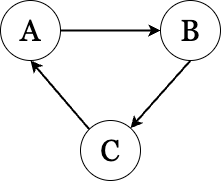
\includegraphics[width=0.6\textwidth,height=\textheight]{img/original_DCG.png}

}

\subcaption{\label{fig-examplegraphs-1}Example graph \(\mathcal{G}\)}

\end{minipage}%
%
\begin{minipage}{0.33\linewidth}

\centering{

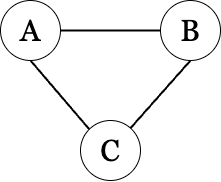
\includegraphics[width=0.6\textwidth,height=\textheight]{img/FCI_graph.png}

}

\subcaption{\label{fig-examplegraphs-2}Corresponding MAAG}

\end{minipage}%
%
\begin{minipage}{0.33\linewidth}

\centering{

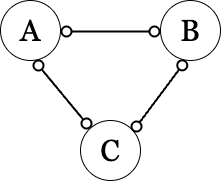
\includegraphics[width=0.6\textwidth,height=\textheight]{img/CCI_graph.png}

}

\subcaption{\label{fig-examplegraphs-3}Corrsponding PAG}

\end{minipage}%

\caption{\label{fig-examplegraphs}\textbf{\emph{Example graph
\(\mathcal{G}\) featuring a cycle and the corresponding MAAG from CCI
and PAG from FCI.}}}

\end{figure}%

The graph produced by the PC algorithm is a \emph{CPDAG} (completed
partially directed acyclic graph), where directed edges (\(A\) → \(B\))
indicate that \(A\) is a direct cause (parent) of \(B\). Unlike FCI and
CCI, the CPDAG does not include circle symbols. Instead, when the PC
algorithm cannot determine the direction of causality, it represents
this uncertainty with bidirectional arrows. While the PC algorithm
serves as a useful reference, its strict assumptions --- acyclicity and
the absence of latent confounders---limit its applicability in more
complex scenarios. For this reason, our primary focus remains on the
results obtained from FCI and CCI, with all PC algorithm results
provided in Section~\ref{sec-pc} for completeness.

\subsection{Precariousness Domains Based on Elsenburg et
al.~(2025)}\label{precariousness-domains-based-on-elsenburg-et-al.-2025}

\textcolor{BrickRed}{We began from the domain definitions and candidate indicators in}
Elsenburg et al. (2025),
\textcolor{BrickRed}{listed below. Before graph learning, we screened candidates for measurement quality and within-domain coherence among precariousness indicators (e.g., missingness, variability, and inter-item correlations). Indicators that were largely disconnected from the remaining precariousness indicators were not carried forward, because they primarily entered as isolated variables while substantially increasing computational cost.}

\begin{enumerate}
\def\labelenumi{\arabic{enumi}.}
\tightlist
\item
  EMPLOYMENT PRECARIOUSNESS
\end{enumerate}

\begin{itemize}
\tightlist
\item
  \texttt{H1\_Arbeidsparticipatie}: Working status
\item
  \texttt{H1\_WerkSit}: Which work situation most applies to you?
\item
  \texttt{H1\_RecentErv8}: Experiences past 12 months: h. You were
  sacked from your job or became unemployed (\emph{reverse})
\end{itemize}

\begin{enumerate}
\def\labelenumi{\arabic{enumi}.}
\setcounter{enumi}{1}
\tightlist
\item
  FINANCIAL PRECARIOUSNESS
\end{enumerate}

\begin{itemize}
\tightlist
\item
  \texttt{H1\_InkHhMoeite}: During the past year, did you have problems
  managing your household income?
\item
  \texttt{H1\_RecentErv9}: Experiences past 12 months: i. You had a
  major financial crisis (\emph{reverse})
\end{itemize}

\begin{enumerate}
\def\labelenumi{\arabic{enumi}.}
\setcounter{enumi}{2}
\tightlist
\item
  HOUSING PRECARIOUSNESS
\end{enumerate}

\begin{itemize}
\tightlist
\item
  \texttt{veilig\_2012}: Score safety (veiligheid) in 2012
  (\emph{reverse})
\item
  \texttt{vrz\_2012}: Score level of resources (niveau voorzieningen) in
  2012 (\emph{reverse})
\item
  \texttt{P\_HUURWON}: Percentage Huurwoningen
\end{itemize}

\begin{enumerate}
\def\labelenumi{\arabic{enumi}.}
\setcounter{enumi}{3}
\tightlist
\item
  CULTURAL PRECARIOUSNESS
\end{enumerate}

\begin{itemize}
\tightlist
\item
  \texttt{H1\_Discr\_sumscore}: Perceived discrimination: sum score of 9
  items (range 9-45)
\item
  \texttt{H1\_SBSQ\_meanscore}: Health literacy: SBSQ meanscore (range
  1-5) (\emph{reverse})
\item
  \texttt{A\_BED\_RU}: Aantal bedrijfsvestigingen; cultuur, recreatie,
  overige diensten (\emph{reverse})
\end{itemize}

\begin{enumerate}
\def\labelenumi{\arabic{enumi}.}
\setcounter{enumi}{4}
\tightlist
\item
  SOCIAL PRECARIOUSNESS
\end{enumerate}

\begin{itemize}
\tightlist
\item
  \texttt{H1\_RecentErv5}: Experiences past 12 months: e. Your steady
  relationship ended (\emph{reverse})
\item
  \texttt{H1\_RecentErv6}: Experiences past 12 months: f.~A long-term
  friendship with a good friend or family member was broken off
  (\emph{reverse})
\item
  \texttt{H1\_RecentErv7}: Experiences past 12 months: g. You had a
  serious problem with a good friend or family member, or neighbour
  (\emph{reverse})
\item
  \texttt{H1\_SSQT}: SSQT (frequency of social contact): sum score of 5
  items (range 5-20) (\emph{reverse})
\item
  \texttt{H1\_SSQSa}: SSQS (adequacy of social contact): sum score of 5
  items, category 3 and 4 not combined (range 5-20) (\emph{reverse})
\end{itemize}

\begin{center}

\includegraphics{draft_v3_SSM_anonymized_LE_KS_files/figure-pdf/unnamed-chunk-12-1.pdf}
\end{center}

\begin{itemize}
\item
  \textbf{High} Correlations: \texttt{emp\_stat} (employment status) and
  \texttt{work\_sit} (work situation) have a strong positive correlation
  of 0.82. This suggests that individuals with higher employment status
  tend to have more secure or favorable work situations.
  \texttt{soc\_freq} (social contact frequency) shows a strong positive
  correlation with \texttt{soc\_adq} (social adequacy) at 0.61. This
  indicates that individuals with more frequent social contact also tend
  to have higher perceived adequacy of social interactions.
\item
  \textbf{Moderate} Correlations: \texttt{nb\_safe} (neighborhood
  safety) and \texttt{nb\_res} (resources) have a moderate positive
  correlation of 0.39, suggesting that areas with higher safety also
  have better resources. \texttt{hea\_lit} (health literacy) has
  moderate correlations with \texttt{emp\_stat} (0.26) and
  \texttt{work\_sit} (0.25), which could mean that higher health
  literacy is associated with better employment situations.
  \texttt{frd\_brk12} (friendship breakups) and \texttt{conf12}
  (conflicts) have a notable correlation of 0.43, indicating a
  relationship between having conflicts and friendship losses.
\item
  \textbf{Low to Moderate} Correlations in Financial Precariousness:
  \texttt{inc\_dif} (income difficulties) has a moderate correlation
  with \texttt{fincri12} (financial crisis) at 0.49. This aligns with
  the expected relationship, where individuals who experience general
  income difficulties are more likely to report financial crises.
\item
  \textbf{Low} Correlations (0.1 - 0.2): Many variables, such as
  \texttt{discrim} (discrimination), \texttt{unemp12} (unemployment
  experience), and \texttt{rel\_end12} (relationship end), have low
  correlations with other variables, suggesting relatively independent
  relationships in the context of this dataset.
\end{itemize}

\subsubsection{Exploratory Factor Analysis
(EFA)}\label{exploratory-factor-analysis-efa}

\begin{center}

\includegraphics[width=0.55\textwidth,height=\textheight]{draft_v3_SSM_anonymized_LE_KS_files/figure-pdf/unnamed-chunk-13-1.pdf}
\end{center}

\begin{center}

\includegraphics[width=0.7\textwidth,height=\textheight]{draft_v3_SSM_anonymized_LE_KS_files/figure-pdf/unnamed-chunk-14-1.pdf}
\end{center}

\paragraph{Factor Loadings (Pattern
Matrix)}\label{factor-loadings-pattern-matrix}

\begin{itemize}
\tightlist
\item
  \textbf{MR1}: High loadings on \texttt{emp\_stat} and
  \texttt{work\_sit} suggest this factor captures \emph{employment}
  precariousness.
\item
  \textbf{MR2}: Strong loadings on \texttt{soc\_freq} and
  \texttt{soc\_adq} indicate \emph{social} precariousness.
\item
  \textbf{MR3}: Key items like \texttt{frd\_brk12}, \texttt{conf12}, and
  \texttt{fincri12}, suggest recent \emph{stressful events}.
\item
  \textbf{MR4}: High loadings on \texttt{nb\_res} and \texttt{cul\_rec}
  may reflect \emph{community resources} precariousness.
\item
  \textbf{MR5}: Variables \texttt{nb\_safe} and \texttt{nb\_rent} with
  high loadings indicate \emph{housing} precariousness.
\end{itemize}

\paragraph{Variance Explained}\label{variance-explained}

The factors cumulatively explain \textbf{38\%} of the variance, with MR1
being the most influential factor. Each factor contributes a smaller
proportion to the total variance (MR1 at 12\%, MR2 at 9\%, etc.).

\paragraph{Factor Intercorrelations}\label{factor-intercorrelations}

Factors are moderately correlated, especially between \emph{MR1 and
MR5}, and \emph{MR2 and MR3}. This indicates that while distinct, these
factors are related---reasonable in a complex socio-economic context.

\paragraph{Model Fit Statistics}\label{model-fit-statistics}

RMSEA (0.071) suggest an acceptable fit. Tucker Lewis Index (0.802)
suggests moderate reliability for the model.

\paragraph{Summary}\label{summary}

The 5-factor model appears interpretable and captures distinct
dimensions of precariousness: \emph{employment, social, stressors,
community resources, and housing precariousness}. Although the overall
fit and explained variance could be stronger, these factors offer
insights into the underlying structure of the data, highlighting key
areas of precariousness.

\subsubsection{PCA}\label{pca}

\begin{center}

\includegraphics[width=0.7\textwidth,height=\textheight]{draft_v3_SSM_anonymized_LE_KS_files/figure-pdf/unnamed-chunk-15-1.pdf}
\end{center}

\begin{itemize}
\tightlist
\item
  Component Retention: The scree plot shows a clear ``elbow'' after the
  first component. This steep drop suggests that most variance is
  explained by the first component. After Dimension 5, the percentage of
  explained variance decreases slightly more gradually, indicating
  diminishing returns for adding more components. If we need to choose
  multiple components, retaining the first 5 components seems
  reasonable, as they capture most of the variance (cumulatively
  explaining about 54.7\% of the total variance).
\end{itemize}

\begin{center}

\includegraphics{draft_v3_SSM_anonymized_LE_KS_files/figure-pdf/unnamed-chunk-16-1.pdf}
\end{center}

\paragraph{Explained variance (contributions) of
variables}\label{explained-variance-contributions-of-variables}

It shows the importance of variables within each component.

\begin{itemize}
\item
  \textbf{Dim1}: High contributions are observed from
  \texttt{emp\_stat}, \texttt{work\_sit}, \texttt{inc\_dif}, and
  \texttt{fincri12}, suggesting that this dimension captures aspects of
  \emph{employment and financial} security.
\item
  \textbf{Dim2}: While \texttt{emp\_stat} and \texttt{work\_sit} overlap
  with Dim1, the strong contributions from \texttt{frd\_brk12} and
  \texttt{rel\_end12} indicate that this dimension captures a focus on
  \emph{recent relationship stressors}.
\item
  \textbf{Dim3}: \texttt{cul\_rec}, \texttt{nb\_res} have the highest
  contributions, indicating this dimension likely represents
  \emph{community and cultural} factors.
\item
  \textbf{Dim4}: \texttt{soc\_freq} and \texttt{soc\_adq} stand out in
  this dimension, suggesting an emphasis on \emph{social}
  precariousness.
\item
  \textbf{Dim5}: \texttt{nb\_safe} and \texttt{nb\_rent} are the top
  contributors, pointing to \emph{housing} security as key themes in
  this component.
\end{itemize}

\paragraph{Cos² Values}\label{cosuxb2-values}

Cos² (squared cosine) values, or the quality of representation, show how
well each variable is represented by each dimension. where higher cos²
values (closer to 1) indicate better representation of a variable by a
component.

\begin{center}

\includegraphics[width=0.7\textwidth,height=\textheight]{draft_v3_SSM_anonymized_LE_KS_files/figure-pdf/unnamed-chunk-17-1.pdf}
\end{center}

\begin{itemize}
\item
  \textbf{Dim.1}: Variables \texttt{emp\_stat}, \texttt{work\_sit},
  \texttt{inc\_dif}, and \texttt{fincri12} show high cos² values,
  meaning that PC1 primarily captures variations in employment and
  financial difficulties. This component could represent
  \emph{employment \& finance} precariousness.
\item
  \textbf{Dim.2}: Variables \texttt{work\_sit}, \texttt{emp\_stat},
  \texttt{frd\_brk12}, and \texttt{conf12} are well-represented in this
  component, suggesting PC2 captures aspects of \emph{recent
  relationship stressors}.
\item
  \textbf{Dim.3}: Variables \texttt{nb\_res} and \texttt{cul\_rec} load
  strongly on PC3. This may represent community or cultural resources,
  indicating that this component is associated with \emph{neighborhood
  resources}.
\item
  \textbf{Dim.4}: This component has high cos² values for
  \texttt{nb\_res}, \texttt{cul\_rec}, \texttt{soc\_freq}, and
  \texttt{soc\_adq.} While \texttt{nb\_res} and \texttt{cul\_rec} are
  also prominent in PC3, PC4 uniquely captures nuanced differentiation
  in \emph{social} precariousness.
\item
  \textbf{Dim.5}: \texttt{nb\_safe} and \texttt{nb\_rent} are
  well-represented by PC5. This component might capture \emph{housing}
  precariousness.
\end{itemize}

\subsubsection{ICA}\label{ica}

\begin{center}

\includegraphics[width=0.7\textwidth,height=\textheight]{draft_v3_SSM_anonymized_LE_KS_files/figure-pdf/unnamed-chunk-18-1.pdf}
\end{center}

\paragraph{Dominant Variables per
Component:}\label{dominant-variables-per-component}

For each Independent Component (IC), we can identify variables with
\emph{high absolute} values in each column. These values indicate that
the IC captures a strong, independent signal associated with these
variables.

\begin{itemize}
\item
  \textbf{IC1}: \texttt{soc\_freq} and \texttt{soc\_adq} have strong
  negative loadings on this component, indicating that this component
  might represent \emph{social} precariousness.
\item
  \textbf{IC2}: \texttt{frd\_brk12}, \texttt{conf12},
  \texttt{rel\_end12}, \texttt{fincri12} and \texttt{unemp12} have the
  most substantial loadings on this component, all with negative signs.
  This might point to a \emph{recent relational or social stressor}
  component.
\item
  \textbf{IC3}: \texttt{nb\_res} and \texttt{cul\_rec} show notable
  negative loadings, pointing to a focus on \emph{community resource}
  precariousness.
\item
  \textbf{IC4}: High loadings for \texttt{nb\_safe}, \texttt{nb\_rent},
  \texttt{nb\_res}, \texttt{cul\_rec}, and \texttt{discrim} suggest a
  theme of \emph{housing and community-based} precariousness, reflecting
  both safety and social challenges within the neighborhood context.
\item
  \textbf{IC5}: \texttt{emp\_stat} and \texttt{work\_sit} both have
  strong negative loadings on this component, suggesting it captures
  \emph{employment} precariousness.
\end{itemize}

\subsubsection{Hierarchical clustering}\label{hierarchical-clustering}

\paragraph{Using Euclidean distance}\label{using-euclidean-distance}

\begin{itemize}
\tightlist
\item
  Ward.D's method: Minimizes the variance within clusters, producing
  more compact and spherical clusters.
\item
  Single linkage: Groups clusters based on the minimum distance between
  points.
\item
  Complete linkage: Groups clusters based on the maximum distance
  between points.
\item
  Average linkage: Uses the average distance between all pairs of points
  in the two clusters.
\end{itemize}

\begin{figure}

\begin{minipage}{0.50\linewidth}
\begin{center}

\includegraphics{draft_v3_SSM_anonymized_LE_KS_files/figure-pdf/unnamed-chunk-19-1.pdf}
\end{center}
\end{minipage}%
%
\begin{minipage}{0.50\linewidth}
\begin{center}

\includegraphics{draft_v3_SSM_anonymized_LE_KS_files/figure-pdf/unnamed-chunk-19-2.pdf}
\end{center}
\end{minipage}%
\newline
\begin{minipage}{0.50\linewidth}
\begin{center}

\includegraphics{draft_v3_SSM_anonymized_LE_KS_files/figure-pdf/unnamed-chunk-19-3.pdf}
\end{center}
\end{minipage}%
%
\begin{minipage}{0.50\linewidth}
\begin{center}

\includegraphics{draft_v3_SSM_anonymized_LE_KS_files/figure-pdf/unnamed-chunk-19-4.pdf}
\end{center}
\end{minipage}%

\end{figure}%

\subparagraph{Consistent Groupings (Across All or Most
Methods)}\label{consistent-groupings-across-all-or-most-methods}

\begin{itemize}
\item
  \texttt{emp\_stat} and \texttt{work\_sit}: This pair consistently
  clusters together across all linkage methods, suggesting that they are
  closely related variables, likely capturing a similar aspect of the
  data (possibly employment status or employment-related information).
\item
  \texttt{nb\_safe}, \texttt{nb\_res}, and \texttt{nb\_rent}: These
  variables are often grouped closely in several methods (especially
  Ward.D, average, and complete linkage). This suggests a similarity or
  common theme among them, potentially related to neighborhood or
  housing precariousness.
\item
  \texttt{soc\_freq} and \texttt{soc\_adq}: These two variables
  frequently cluster together, indicating they likely measure aspects of
  social frequency and adequacy in similar ways. They appear together in
  Ward.D, average, and complete linkage.
\item
  \texttt{frd\_brk12} and \texttt{conf12}: These variables are often
  clustered closely (though they sometimes join with other variables
  like rel\_end12), suggesting they may capture aspects of relationship
  or social conflict. This pair appears in close proximity, especially
  in average and Ward.D.
\end{itemize}

\subparagraph{Inconsistent Groupings (Variability Across
Methods)}\label{inconsistent-groupings-variability-across-methods}

\begin{itemize}
\item
  \texttt{hea\_lit}: This variable shows inconsistent clustering across
  methods. In Ward.D, it joins with \texttt{fincri12}, while in other
  methods, it's often more isolated or grouped with variables that do
  not appear similar. This may suggest that \texttt{hea\_lit} does not
  strongly correlate with other variables, or it has multidimensional
  aspects affecting its grouping across methods.
\item
  \texttt{discrim}: This variable also shows variable groupings. In
  Ward.D, it is grouped with \texttt{hea\_lit}, while in other methods
  (e.g., complete and single linkage), it clusters differently,
  sometimes on its own. This variability may indicate that
  \texttt{discrim} has weaker associations with the main clusters in the
  data or overlaps partially with multiple clusters.
\item
  Social and Financial Variables (\texttt{inc\_dif}, \texttt{fincri12},
  \texttt{unemp12}): These variables appear together in some methods
  (e.g., Ward.D clusters \texttt{fincri12} and \texttt{inc\_dif}), but
  in others, they are spread out. This inconsistency suggests that
  social and financial variables may not have strong or consistent ties
  across different methods, perhaps due to capturing different aspects
  of precariousness.
\end{itemize}

\subparagraph{Summary}\label{summary-1}

The consistent clusters are likely capturing distinct thematic
dimensions of the data (e.g., employment, housing, social contact),
while the inconsistent variables may reflect multifaceted or weakly
correlated attributes that do not fit neatly into one cluster.

\paragraph{Using Mutual Information}\label{using-mutual-information}

Using mutual information (MI) as a basis for hierarchical clustering
differs from using traditional distance measures (like Euclidean
distance) in a few key ways.

\begin{center}

\includegraphics[width=0.6\textwidth,height=\textheight]{draft_v3_SSM_anonymized_LE_KS_files/figure-pdf/unnamed-chunk-20-1.pdf}
\end{center}

\subparagraph{Comparison to Euclidean Distance
Clustering}\label{comparison-to-euclidean-distance-clustering}

\begin{itemize}
\item
  \textbf{Housing and Community} Cluster: The variables
  \texttt{nb\_safe}, \texttt{nb\_res}, \texttt{nb\_rent}, and
  \texttt{cul\_rec} cluster together, indicating a strong association
  among housing-related and community-based factors. This suggests a
  shared theme of housing or community precariousness. This grouping is
  also observed in the Euclidean-based clustering, but it appears more
  tightly connected here, potentially due to the non-linear
  relationships highlighted by mutual information.
\item
  \textbf{Employment and Social Support} Cluster: \texttt{emp\_stat} and
  \texttt{work\_sit} form a cluster, linking employment status and work
  situation together as they did in Euclidean-based clustering. These
  remain closely associated regardless of the distance metric used.
  \texttt{soc\_freq} and \texttt{soc\_adq}, related to social contact
  frequency and adequacy, cluster nearby, indicating they have a
  stronger non-linear relationship with employment variables. This is a
  subtle difference as Euclidean distance might not capture this
  association as effectively.
\item
  \textbf{Financial Stressor} Cluster: \texttt{inc\_dif} and
  \texttt{fincri12}, representing income difficulties and recent
  financial crises, consistently cluster together in both approaches,
  showing a strong association, likely linear. However, mutual
  information-based clustering links these financial stressors with
  social support variables, suggesting that financial challenges may
  have complex dependencies with social support in this dataset.
\item
  \textbf{Relational Stressor} Cluster: \texttt{frd\_brk12},
  \texttt{conf12}, \texttt{discrim}, \texttt{hea\_lit},
  \texttt{unemp12}, and \texttt{rel\_end12} form a \emph{looser} cluster
  focused on social and relational stressors (e.g., friendship breakup,
  conflicts, and discrimination). Compared to Euclidean clustering,
  \texttt{discrim} and \texttt{hea\_lit} (health literacy) appear closer
  to relational stressors here, indicating that non-linear relationships
  might play a larger role in linking these variables.
\end{itemize}

\subparagraph{Summary}\label{summary-2}

In conclusion, mutual information-based clustering provides an
alternative perspective that can reveal more intricate associations
between variables, especially for those with non-linear relationships.
Compared to Euclidean clustering, it shows a similar high-level
structure but emphasizes nuanced connections between variables,
particularly around social support, employment, and financial stress.

\subsubsection{Conclusions on Precariousness
factors}\label{conclusions-on-precariousness-factors}

\textcolor{BrickRed}{Based on the consistent findings across multiple analyses, we excluded the variables}
\texttt{discrim}, \texttt{hea\_lit}, \texttt{unemp12}, and
\texttt{rel\_end12},
\textcolor{BrickRed}{because they did not map cleanly onto any precariousness domain and showed little association with the remaining precariousness indicators (see the correlation table above). Retaining them would mainly add weakly connected or isolated variables to the subsequent graph learning step and materially increase computational cost, with limited gain in interpretability. Therefore, we propose retaining the following key precariousness factors:}

\begin{itemize}
\tightlist
\item
  Employment Precariousness: \texttt{emp\_stat}, \texttt{work\_sit}
\item
  Social Precariousness: \texttt{soc\_freq}, \texttt{soc\_adq}
\item
  Housing Precariousness: \texttt{nb\_safe}, \texttt{nb\_res},
  \texttt{nb\_rent}, \texttt{cul\_rec}
\item
  Recent Relational Stressors: \texttt{frd\_brk12}, \texttt{conf12}
\item
  Recent Financial Stressors: \texttt{fincri12}, \texttt{inc\_dif}
\end{itemize}

We construct each precariousness factor by calculating the mean value of
the combined variables. Below, we present the updated correlation table
for the newly composed factors, along with the corresponding
distributions of all variables to be used in the causal discovery
analysis.

\begin{center}

\includegraphics{draft_v3_SSM_anonymized_LE_KS_files/figure-pdf/unnamed-chunk-21-1.pdf}
\end{center}

\begin{center}

\includegraphics{draft_v3_SSM_anonymized_LE_KS_files/figure-pdf/unnamed-chunk-22-1.pdf}
\end{center}

\subsection{Results from CCI algorithm}\label{sec-cci}

\begin{figure}

\begin{minipage}{0.50\linewidth}

\centering{


\includegraphics[width=1\textwidth,height=\textheight]{img/CCI_depsum.png}

}

\subcaption{\label{fig-sum-cci-1}CCI MAAG}

\end{minipage}%
%
\begin{minipage}{0.50\linewidth}

\centering{

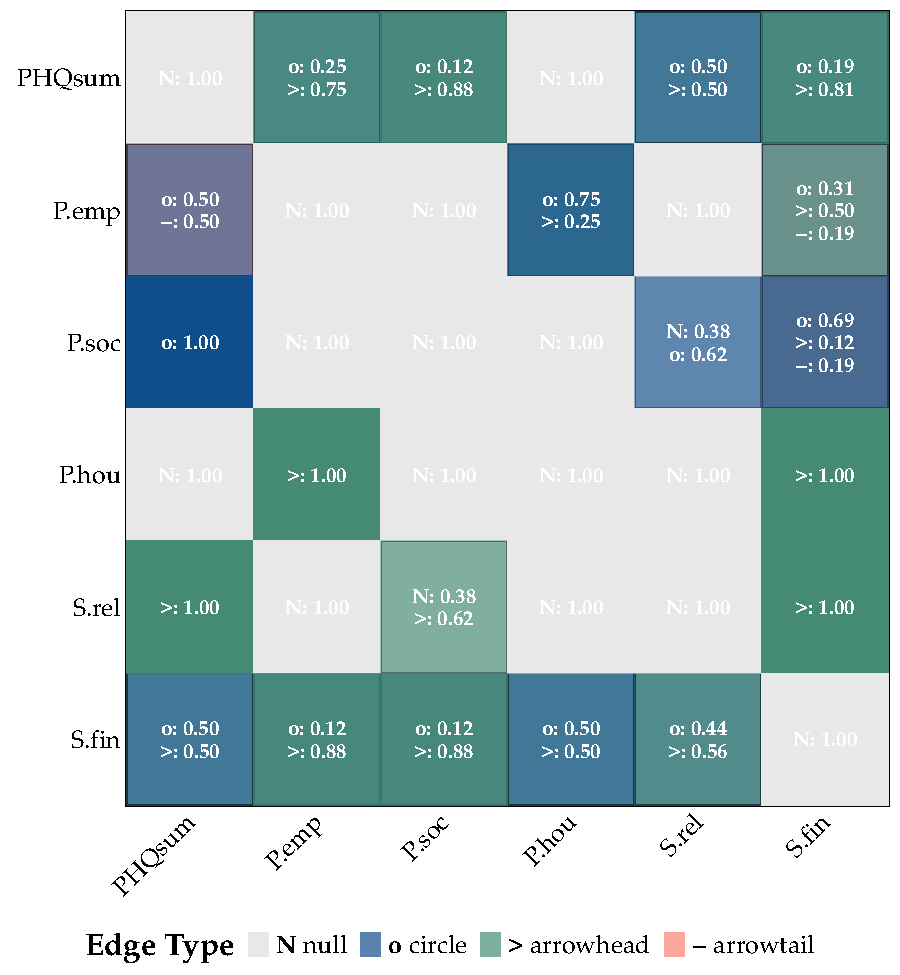
\includegraphics[width=1\textwidth,height=\textheight]{img/depsum_mat_cci.pdf}

}

\subcaption{\label{fig-sum-cci-2}Proportion matrix}

\end{minipage}%

\caption{\label{fig-sum-cci}\textbf{\emph{Causal pathways between
precariousness factors and overall depression severity, estimated with
CCI.}} \textbf{(a)} Aggregated CCI graph (MAAG) summarizing the most
frequent edge types across bootstraps. Compared to FCI, the CCI
algorithm produces more ambiguous orientations, with fewer clear
directional arrows. \textbf{(b)} Proportion matrix showing edge-type
frequencies across bootstraps. More undirected and bidirectional edges
appear relative to FCI, reflecting increased uncertainty and potential
latent confounding in the estimated structure.}

\end{figure}%

\begin{figure}

\begin{minipage}{\linewidth}

\centering{

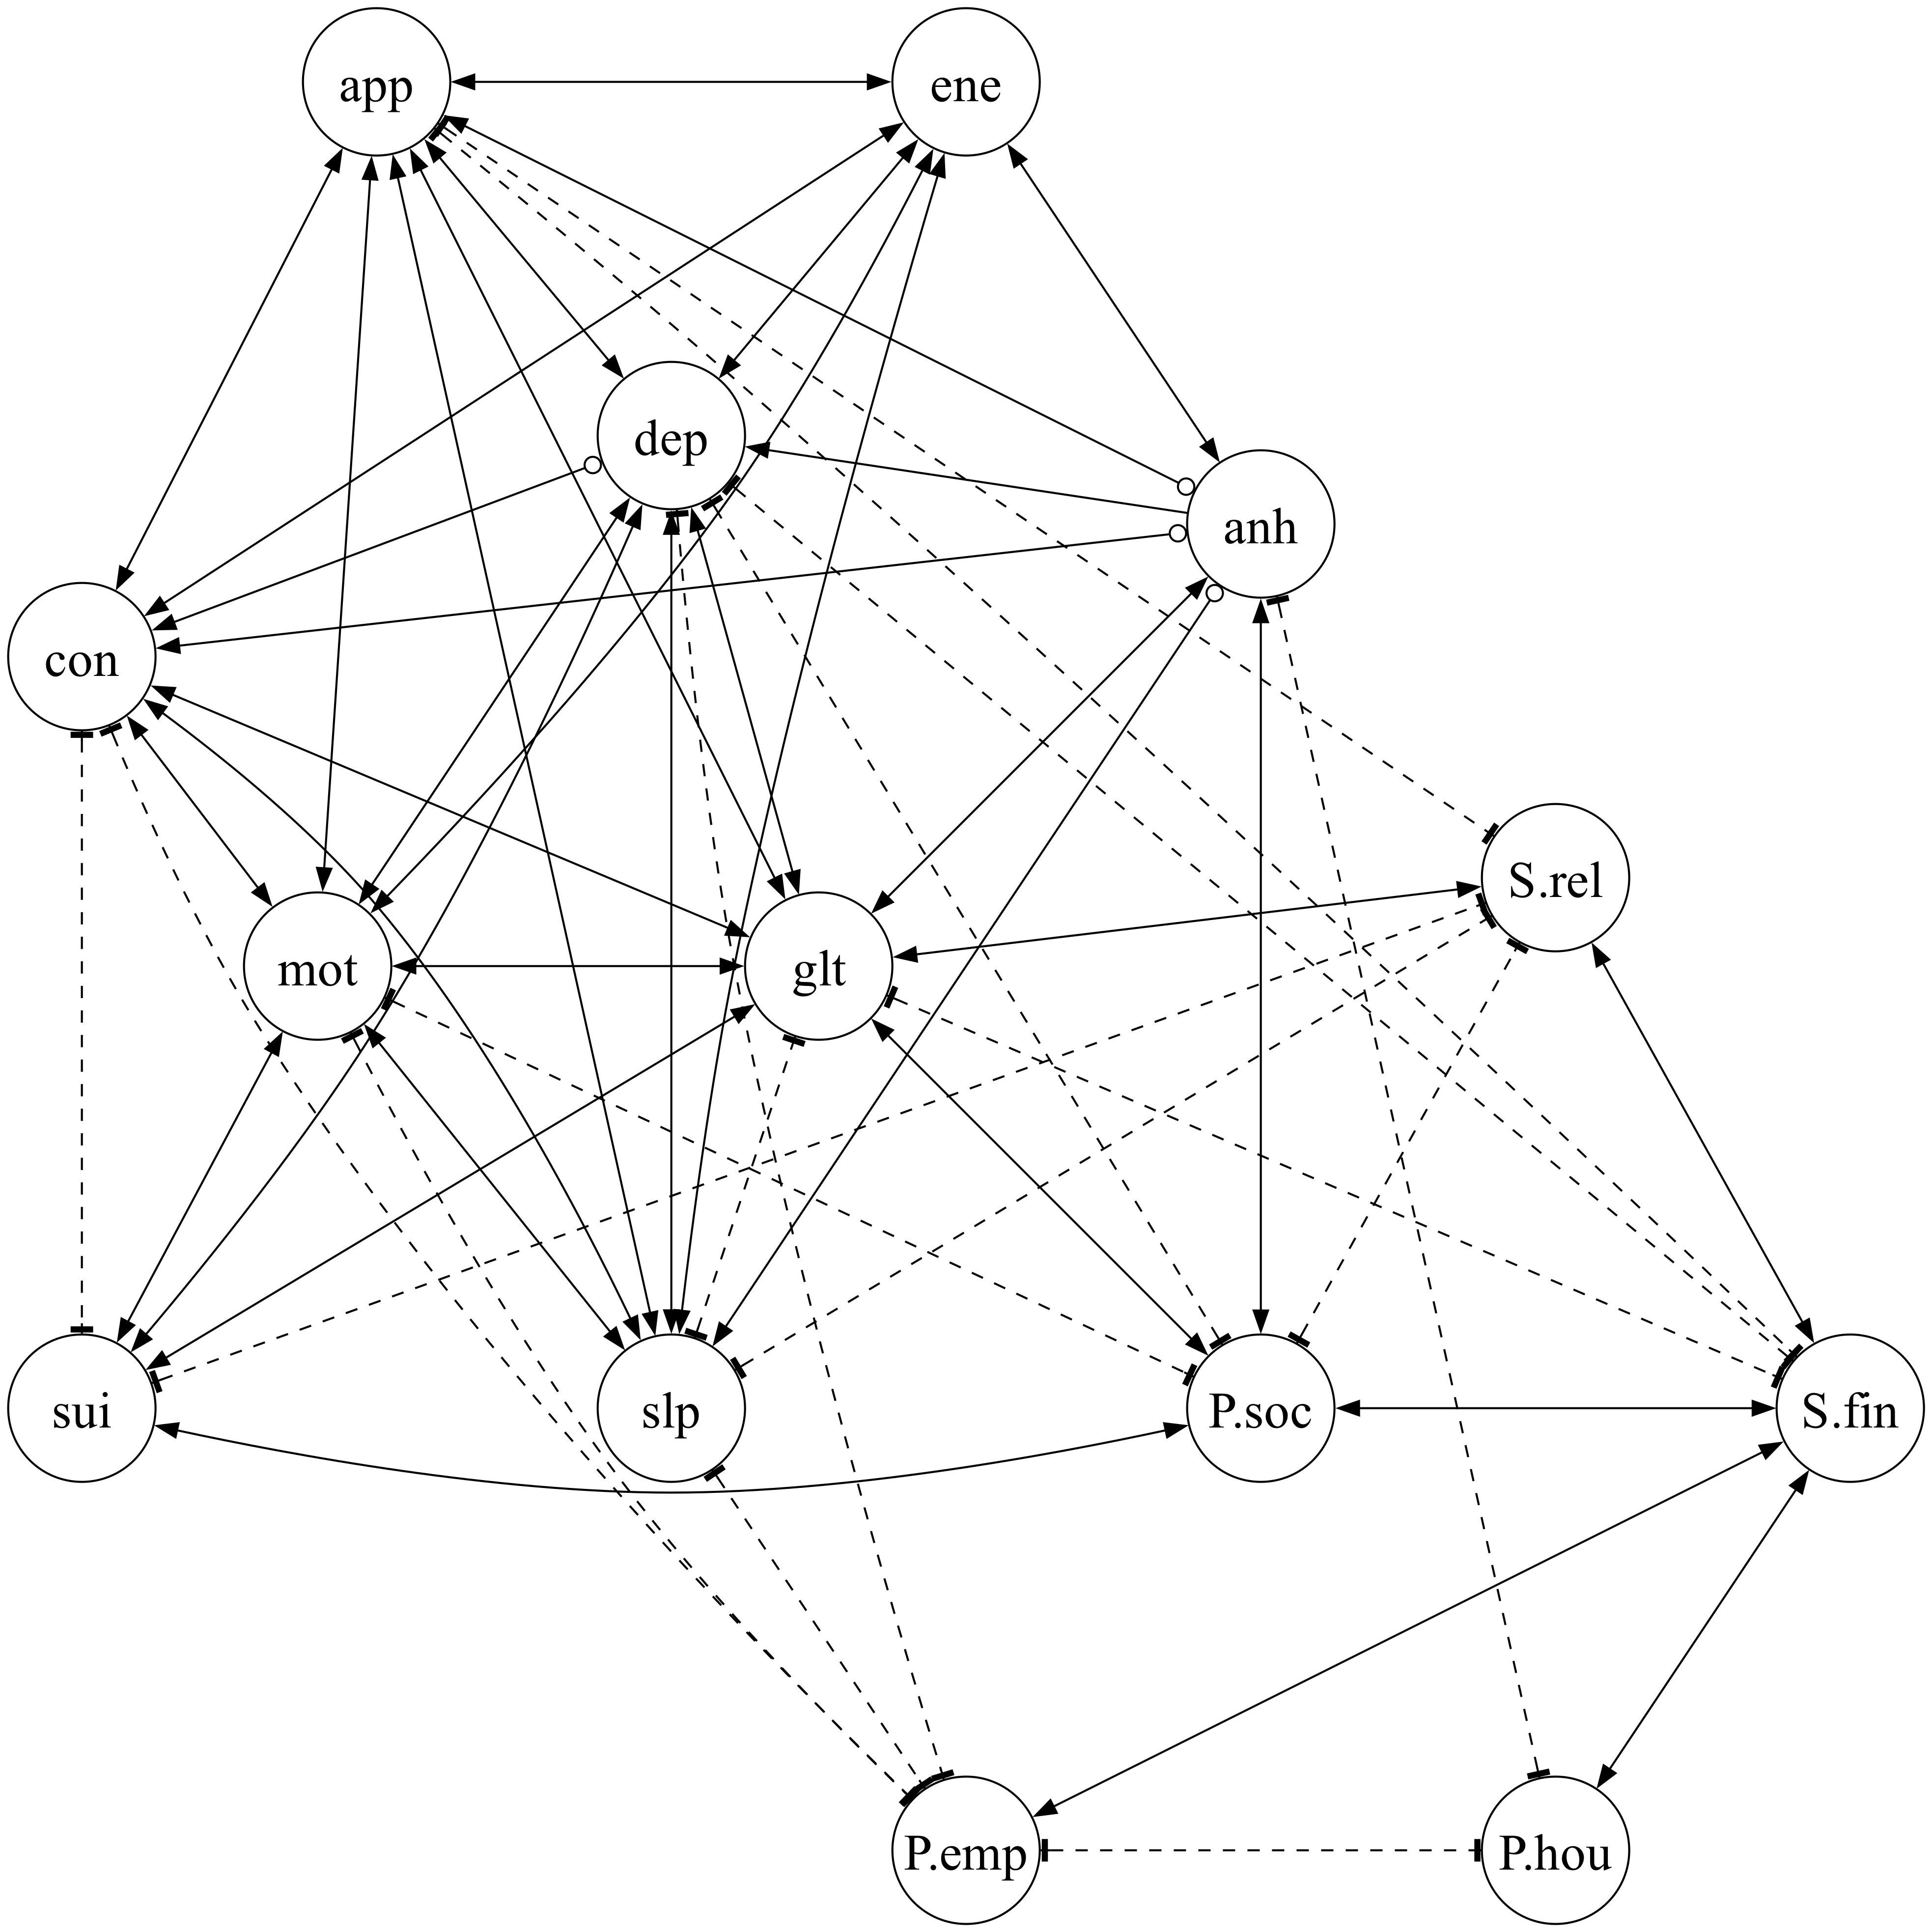
\includegraphics[width=0.6\textwidth,height=\textheight]{img/symptom_graph_CCI.png}

}

\subcaption{\label{fig-sym-cci-1}CCI MAAG}

\end{minipage}%
\newline
\begin{minipage}{\linewidth}

\centering{

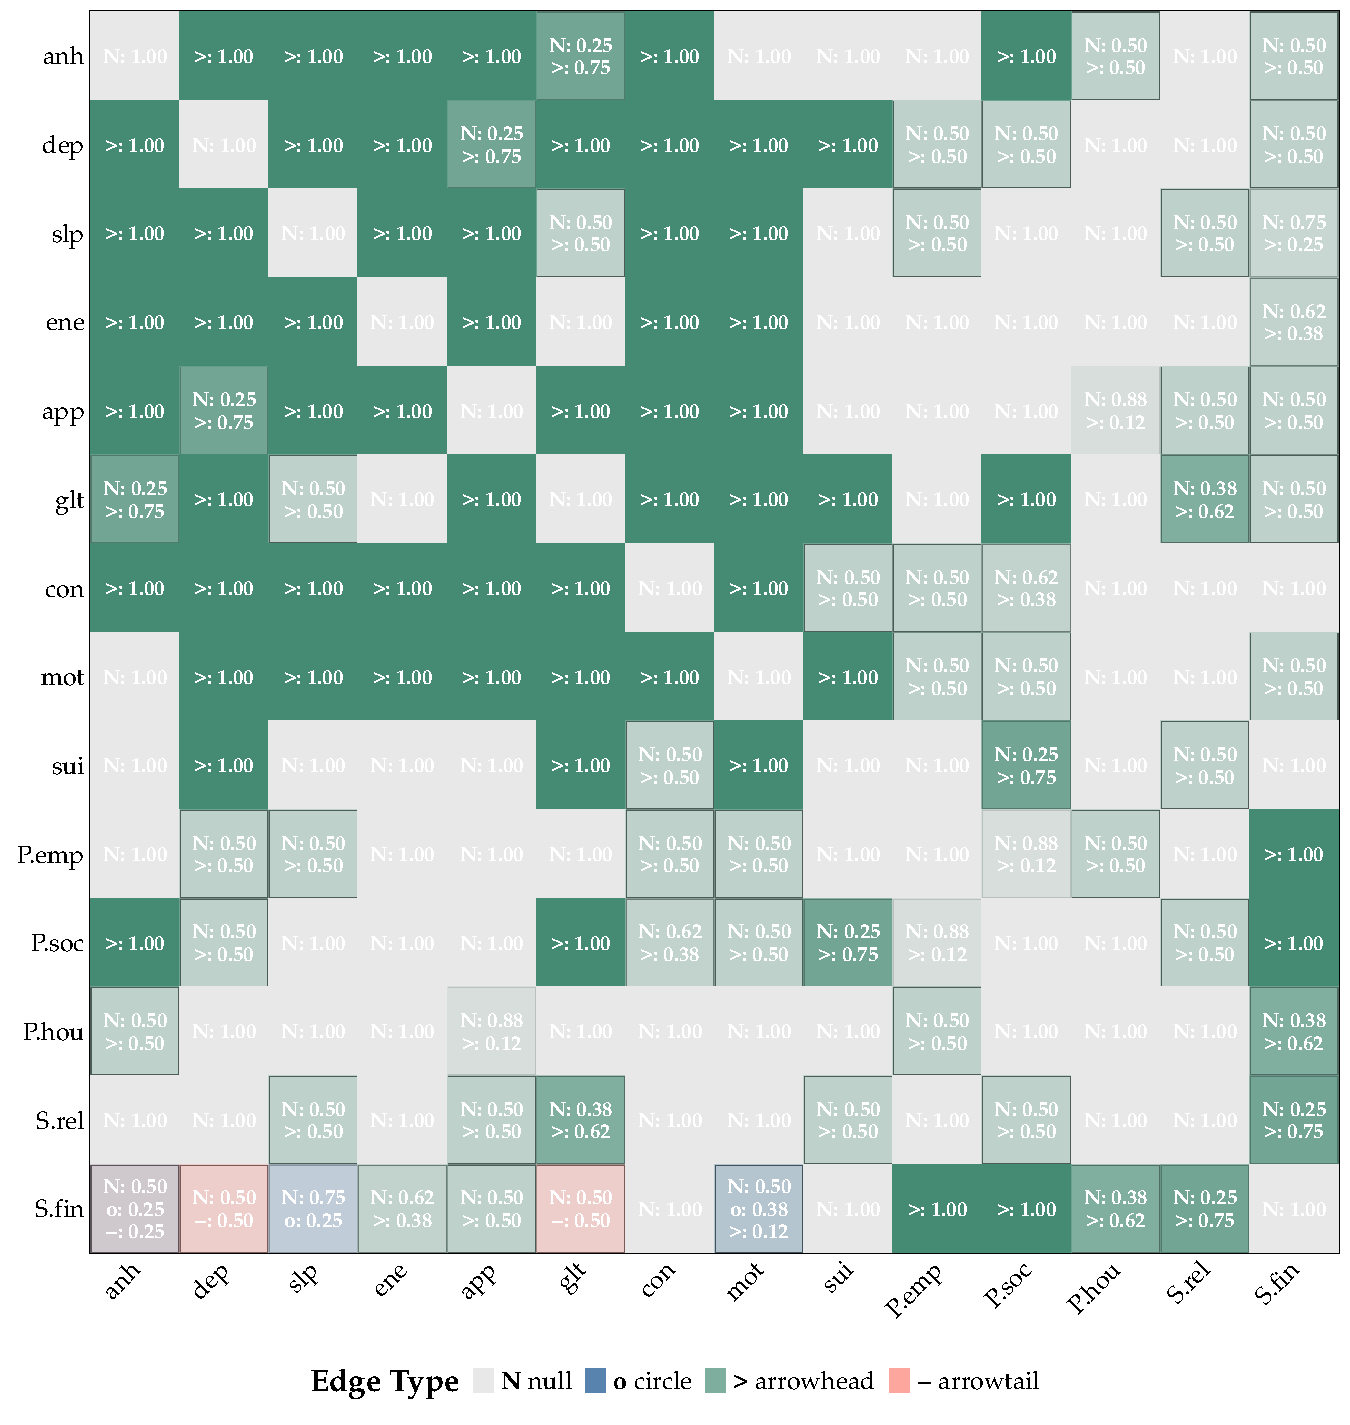
\includegraphics[width=0.6\textwidth,height=\textheight]{img/symptom_mat_cci.pdf}

}

\subcaption{\label{fig-sym-cci-2}Proportion matrix}

\end{minipage}%

\caption{\label{fig-sym-cci}\textbf{\emph{Causal pathways linking
individual depressive symptoms and precariousness factors, estimated
with CCI.}} \textbf{(a)} Aggregated CCI graph (MAAG) summarizing
symptom--precariousness relationships. CCI yields a denser network with
more bidirectional edges, consistent with stronger involvement of latent
confounders. \textbf{(b)} Proportion matrix showing edge-type
frequencies across bootstraps. Compared to FCI, CCI favors arrowheads
more often, resulting in more bidirectional or confounded edges between
symptoms and precariousness factors.}

\end{figure}%

\newgeometry{top=10mm, bottom=20mm, left=40mm, right=40mm}

\begin{figure}

\begin{minipage}{\linewidth}

\centering{

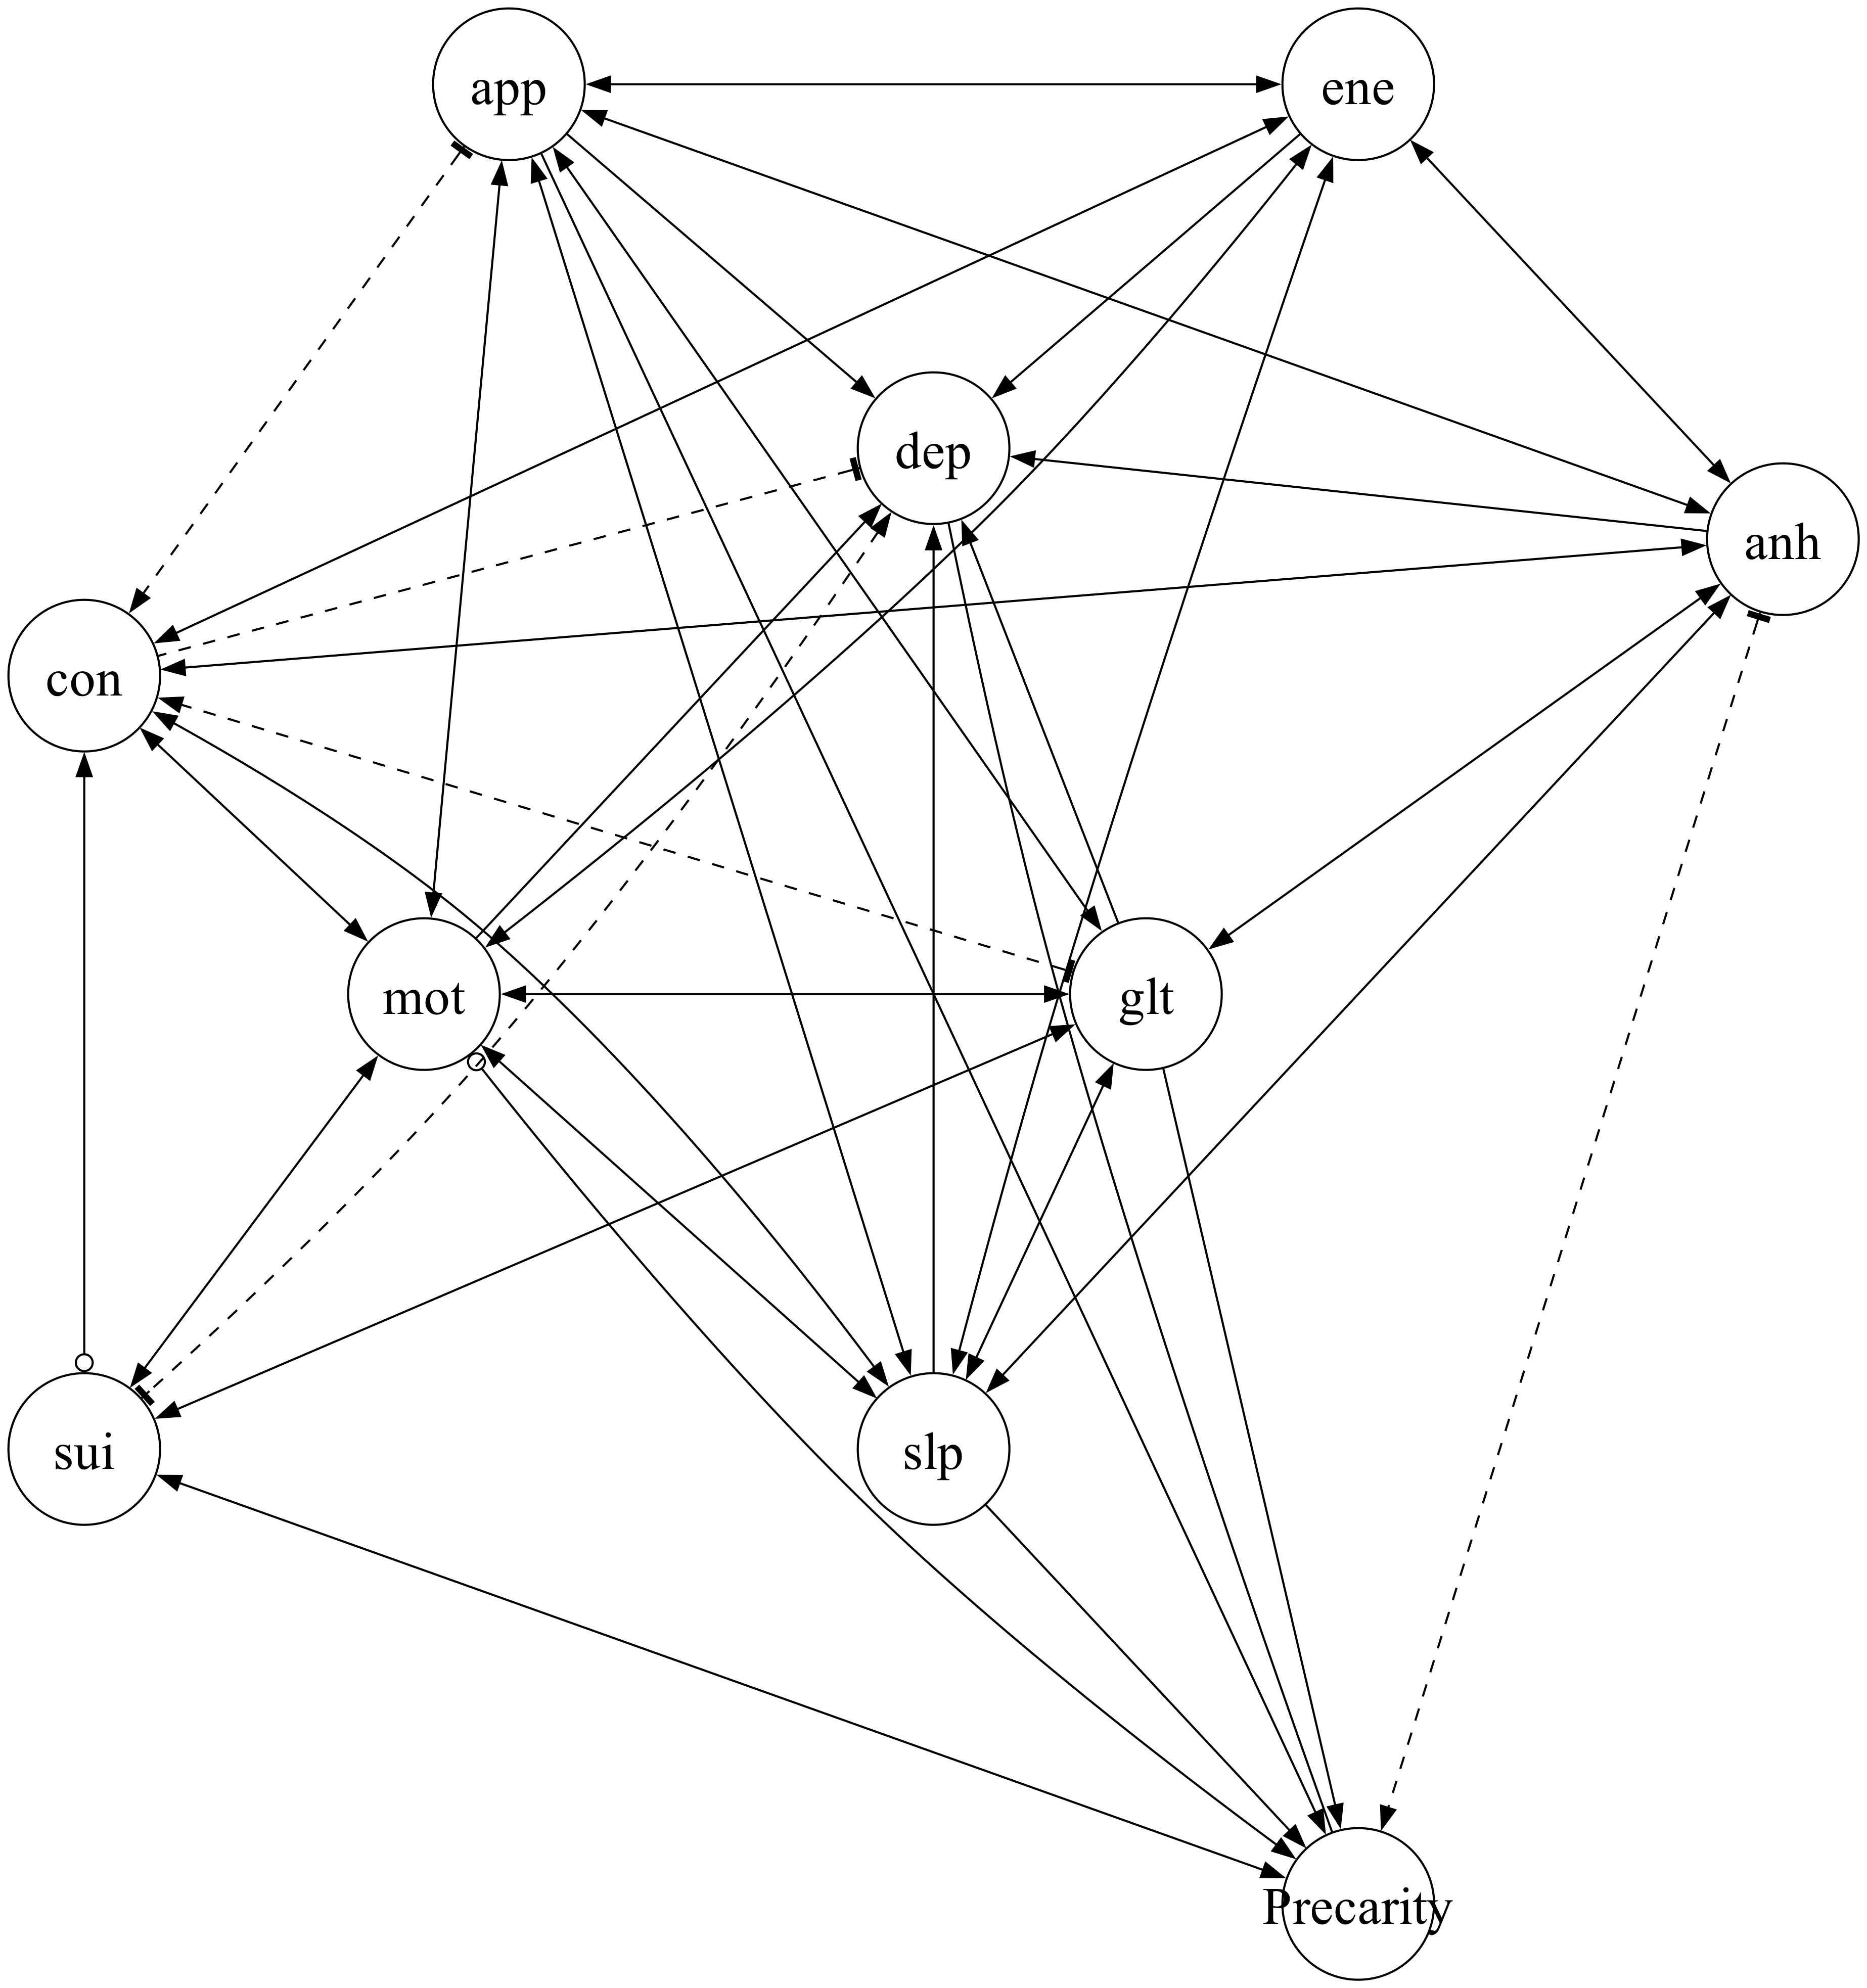
\includegraphics[width=0.6\textwidth,height=\textheight]{img/presum_graph_CCI.png}

}

\subcaption{\label{fig-presum-cci-1}CCI MAAG}

\end{minipage}%
\newline
\begin{minipage}{\linewidth}

\centering{

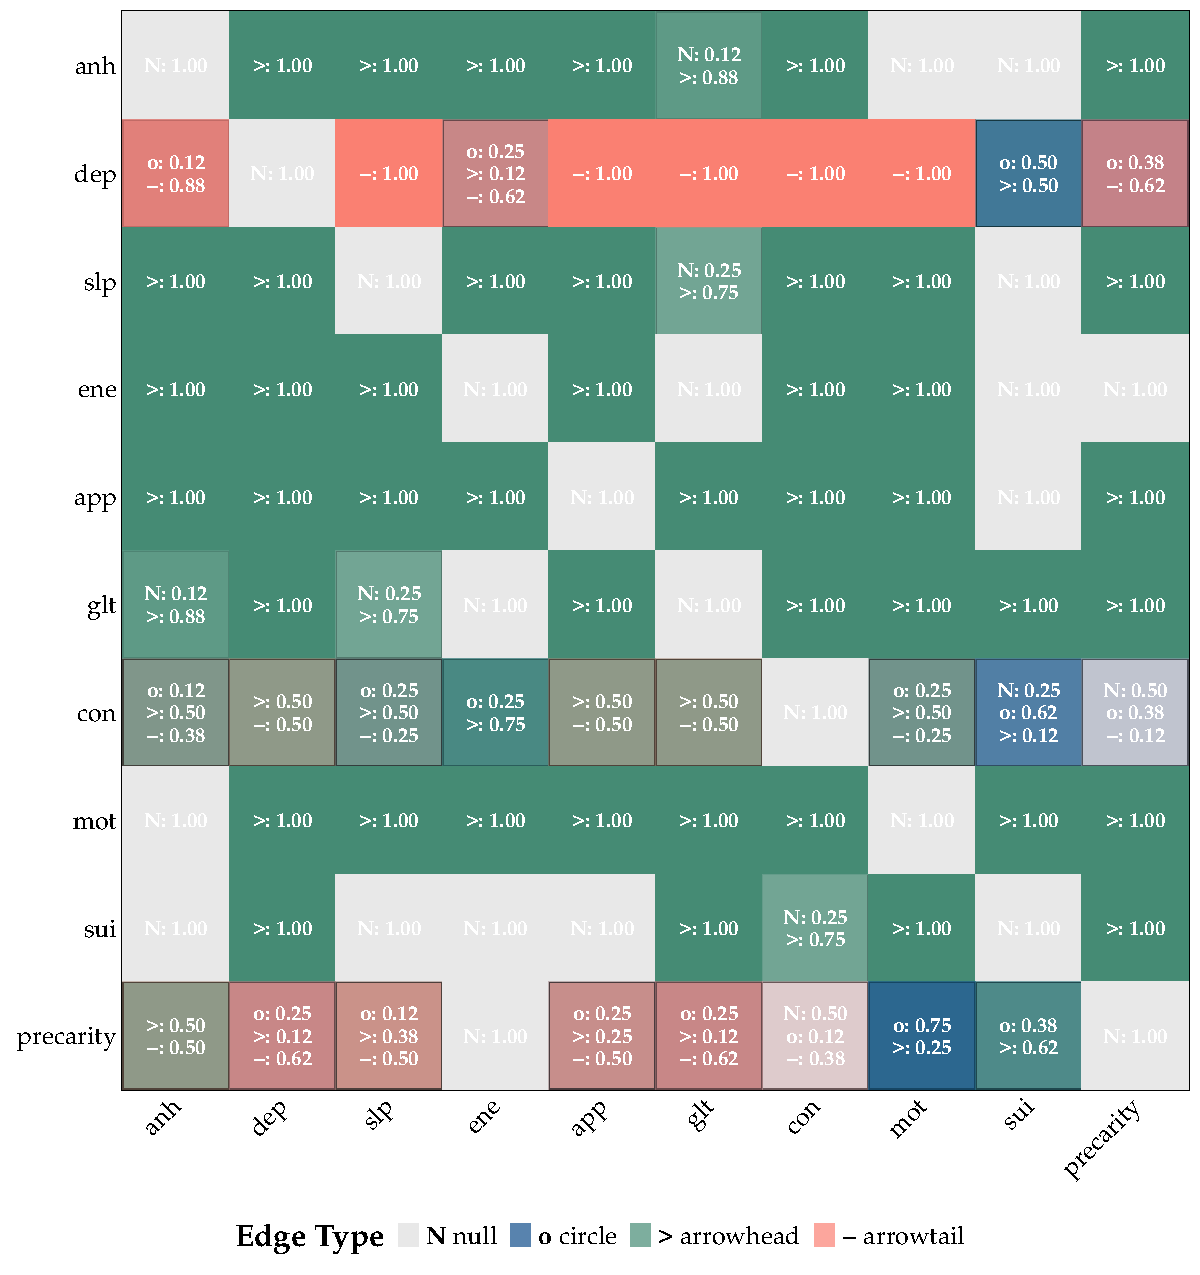
\includegraphics[width=0.6\textwidth,height=\textheight]{img/presum_mat_cci.pdf}

}

\subcaption{\label{fig-presum-cci-2}Proportion matrix}

\end{minipage}%

\caption{\label{fig-presum-cci}\textbf{\emph{Causal pathways between
overall precariousness and individual depressive symptoms, estimated
with CCI.}} \textbf{(a)} Aggregated CCI graph (MAAG) summarizing the
most frequent edge types across bootstraps. CCI suggests stronger
interconnections among symptoms, with more bidirectional links than in
the FCI graph. Depressed mood (\emph{dep}) appears as a distinct
exception, receiving influence from many other symptoms. \textbf{(b)}
Proportion matrix showing edge-type frequencies across bootstraps. CCI
highlights a potential feedback loop between \emph{dep} and overall
precariousness, represented by a tail--tail edge, consistent with a
reinforcing cycle. Compared to FCI, the CCI results emphasize latent
confounding and cyclic dependencies.}

\end{figure}%

\restoregeometry

\subsection{Results from PC algorithm}\label{sec-pc}

\begin{figure}

\begin{minipage}{0.50\linewidth}

\centering{

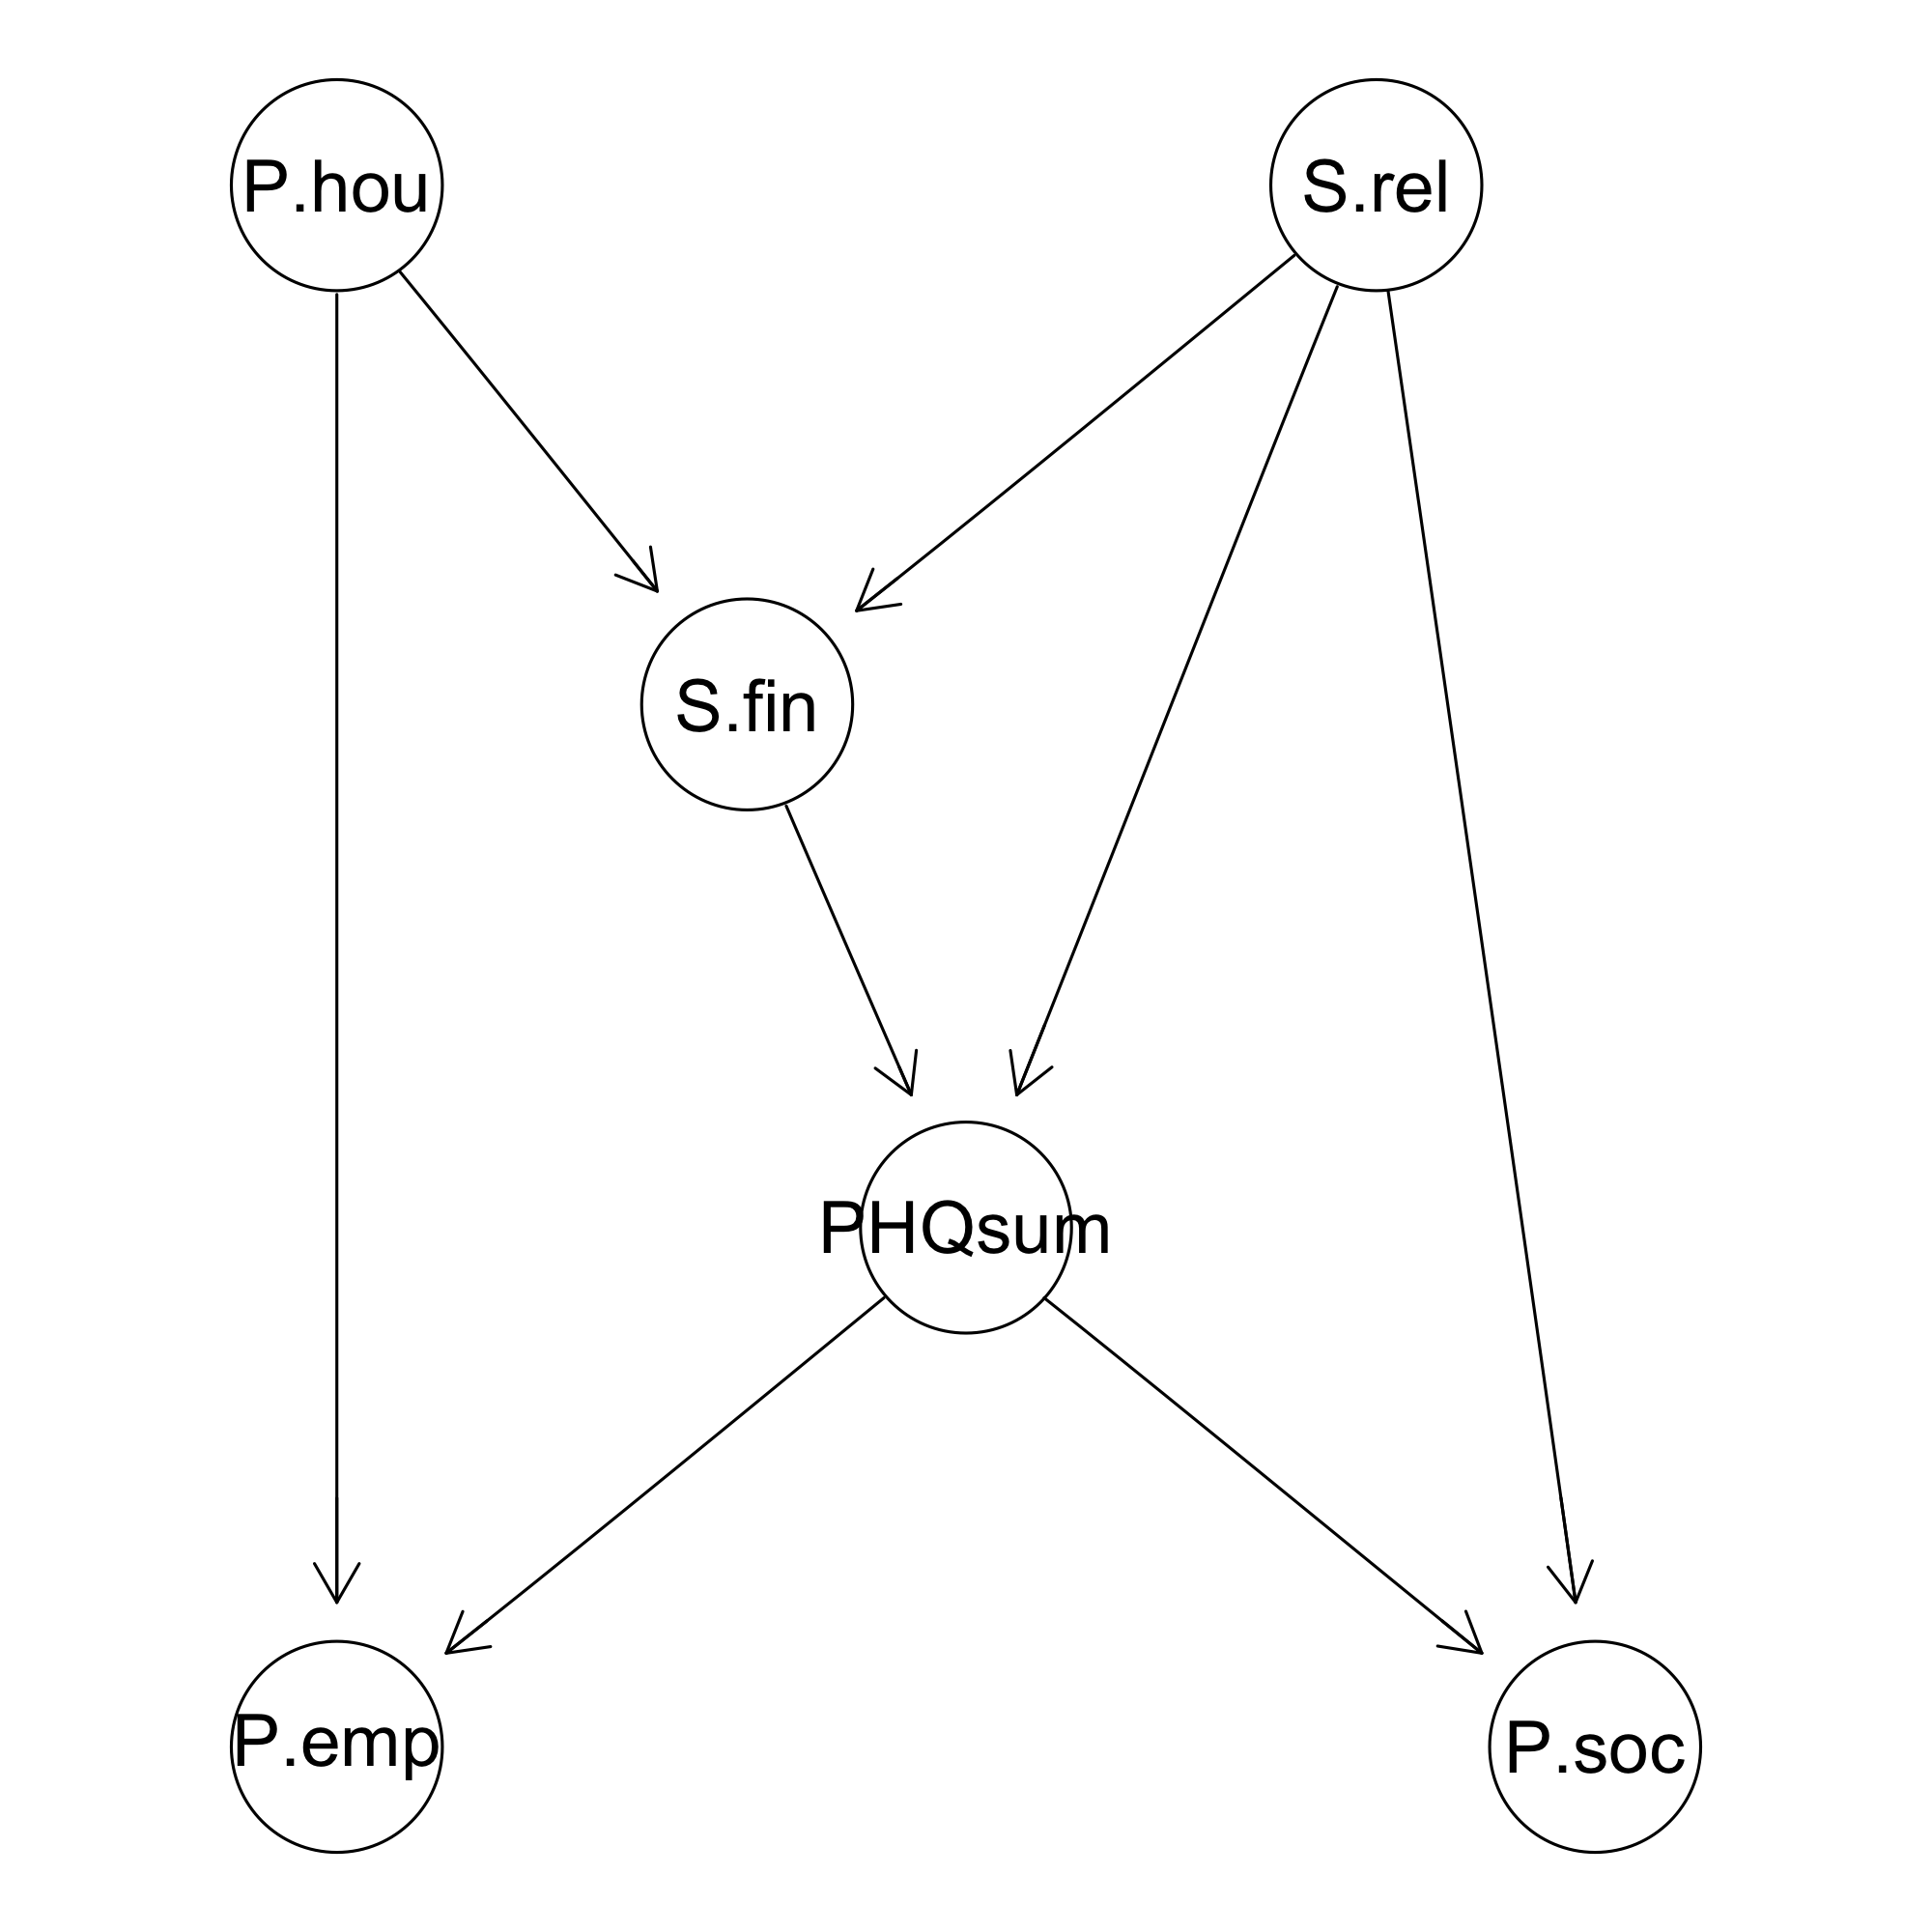
\includegraphics[width=1\textwidth,height=\textheight]{img/sum_PC_all.png}

}

\subcaption{\label{fig-pc_sum-1}Using both GaussianCI and RCoT}

\end{minipage}%
%
\begin{minipage}{0.50\linewidth}

\centering{

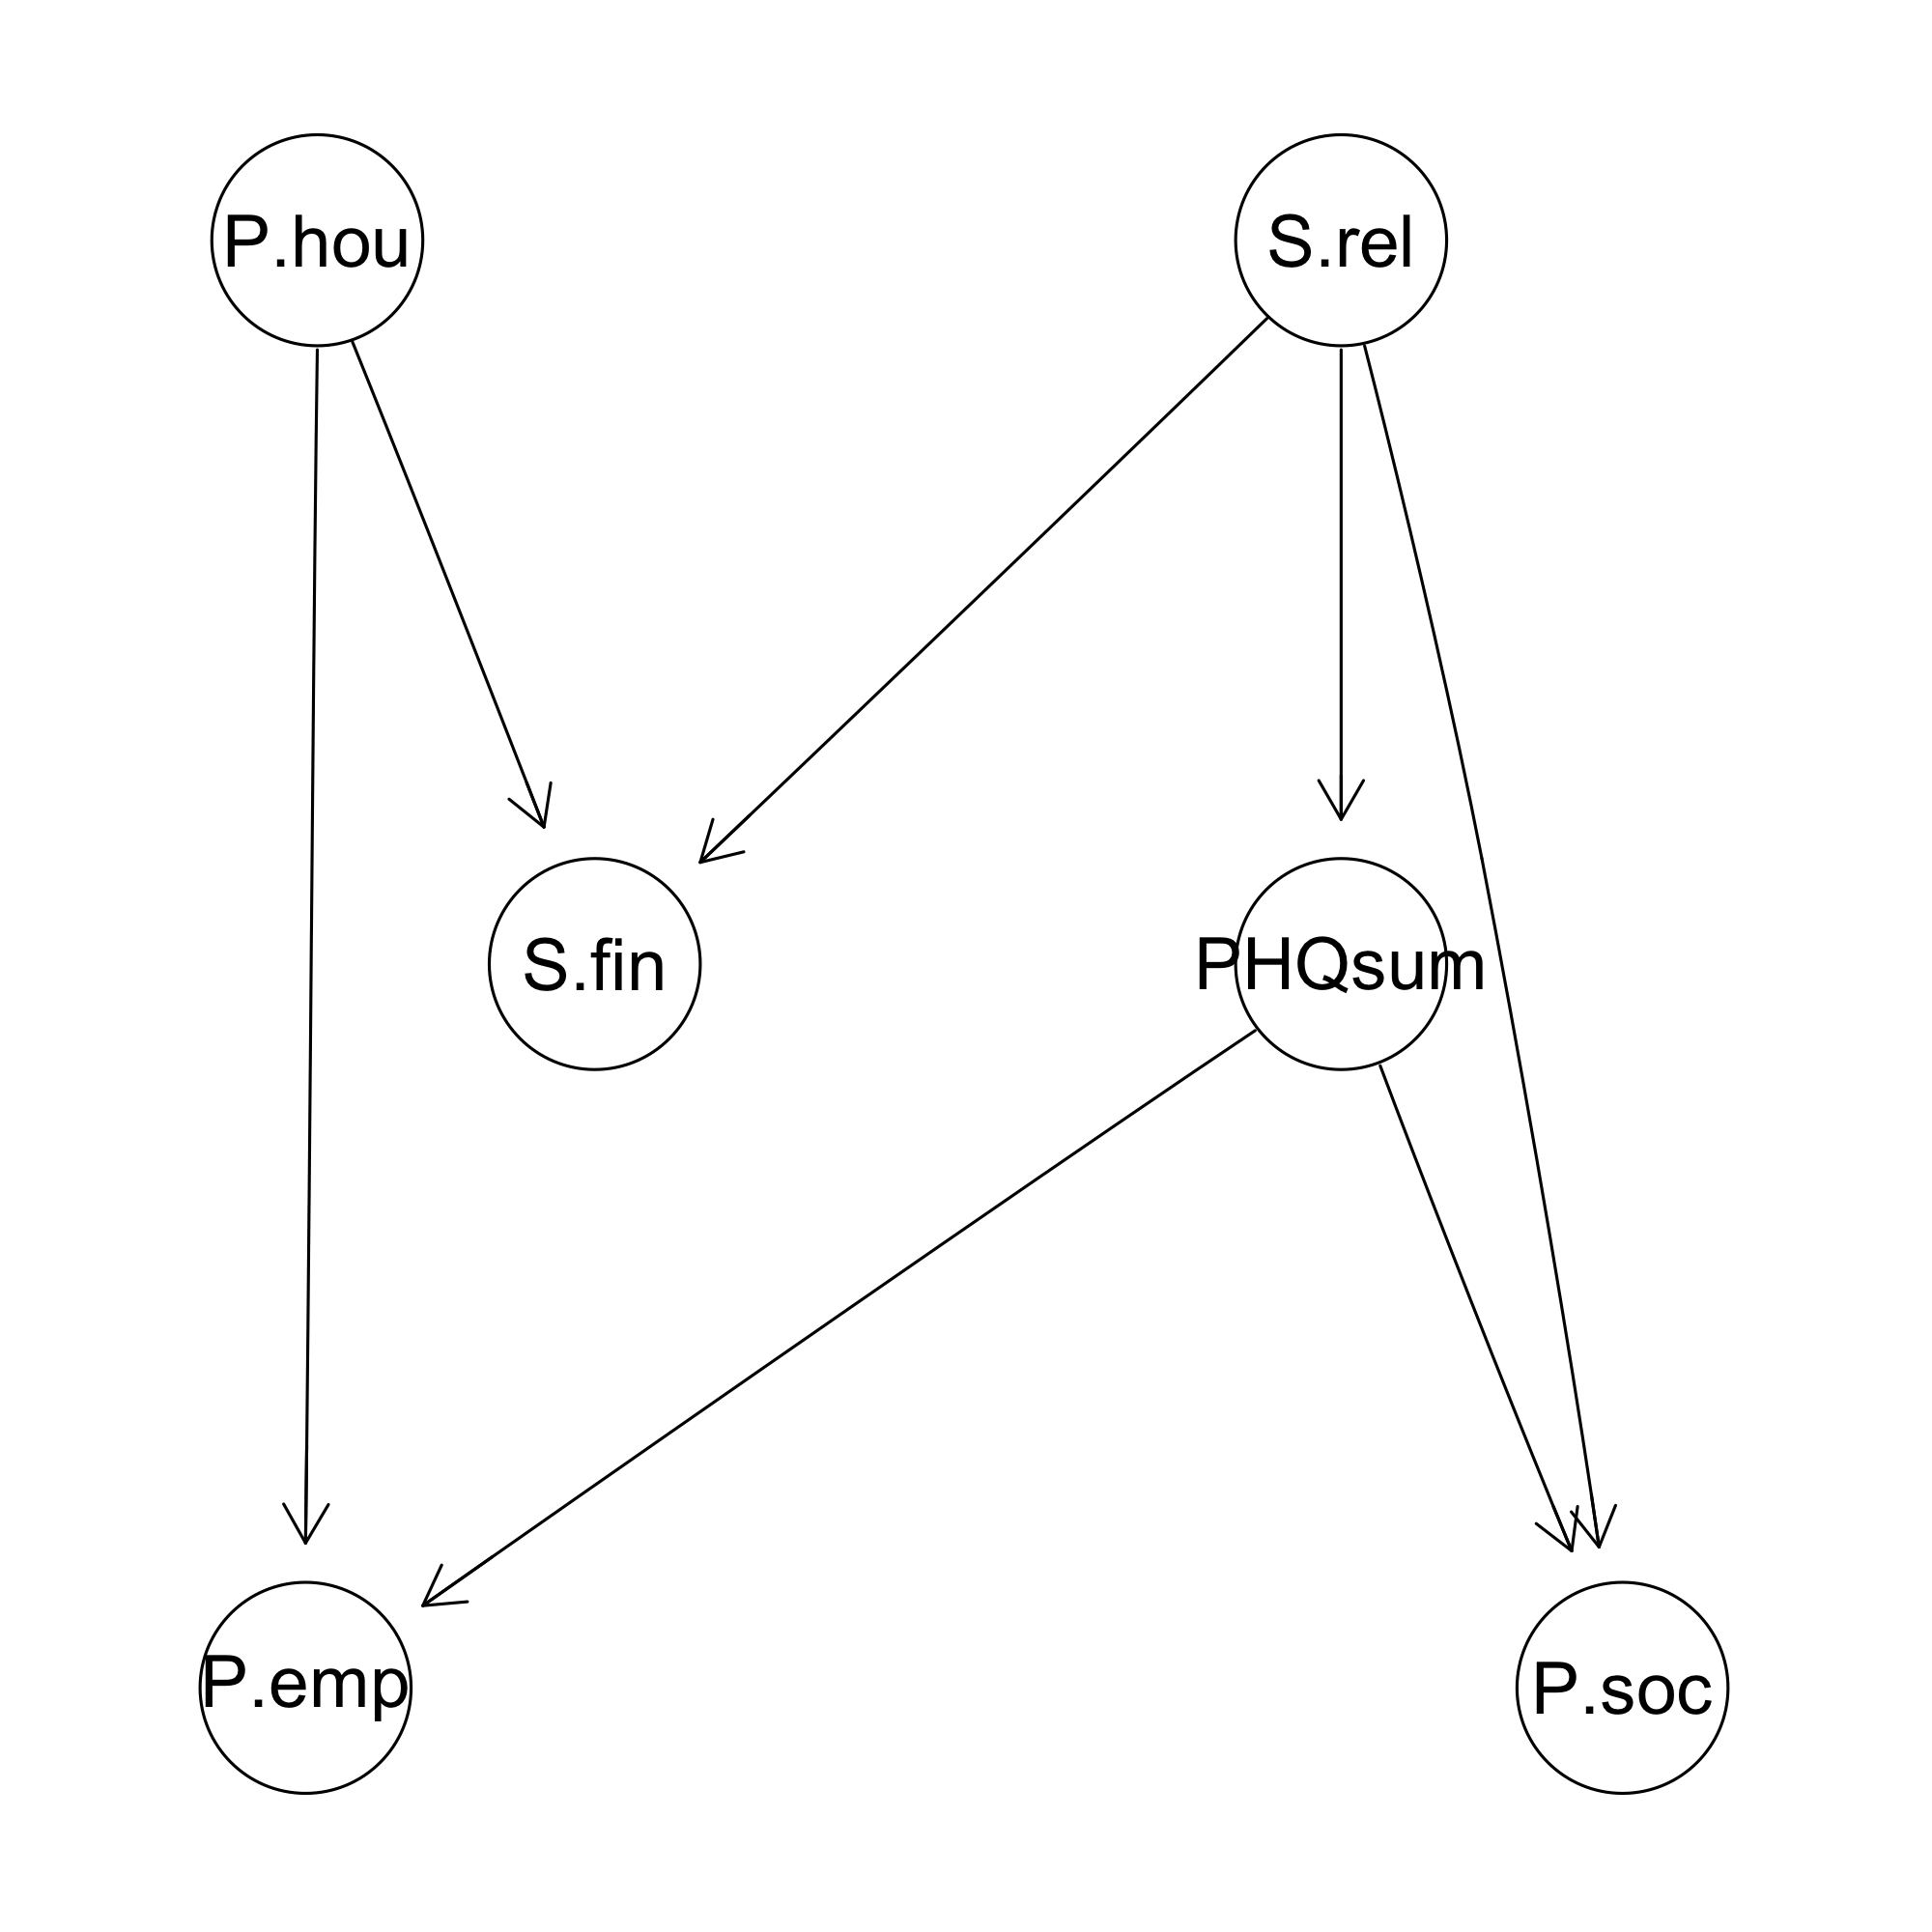
\includegraphics[width=1\textwidth,height=\textheight]{img/sum_PC_RCoTonly.png}

}

\subcaption{\label{fig-pc_sum-2}Using only RCoT}

\end{minipage}%

\caption{\label{fig-pc_sum}\textbf{\emph{Causal pathways between
precariousness factors and overall depression severity, estimated with
PC.}} \textbf{(a)} Graph using both Gaussian CI and RCoT tests.
\textbf{(b)} Graph using only RCoT. PC produces a CPDAG, which excludes
cycles and represents uncertainty with bidirectional edges. Gaussian CI
yields denser graphs than RCoT.}

\end{figure}%

\begin{figure}

\centering{

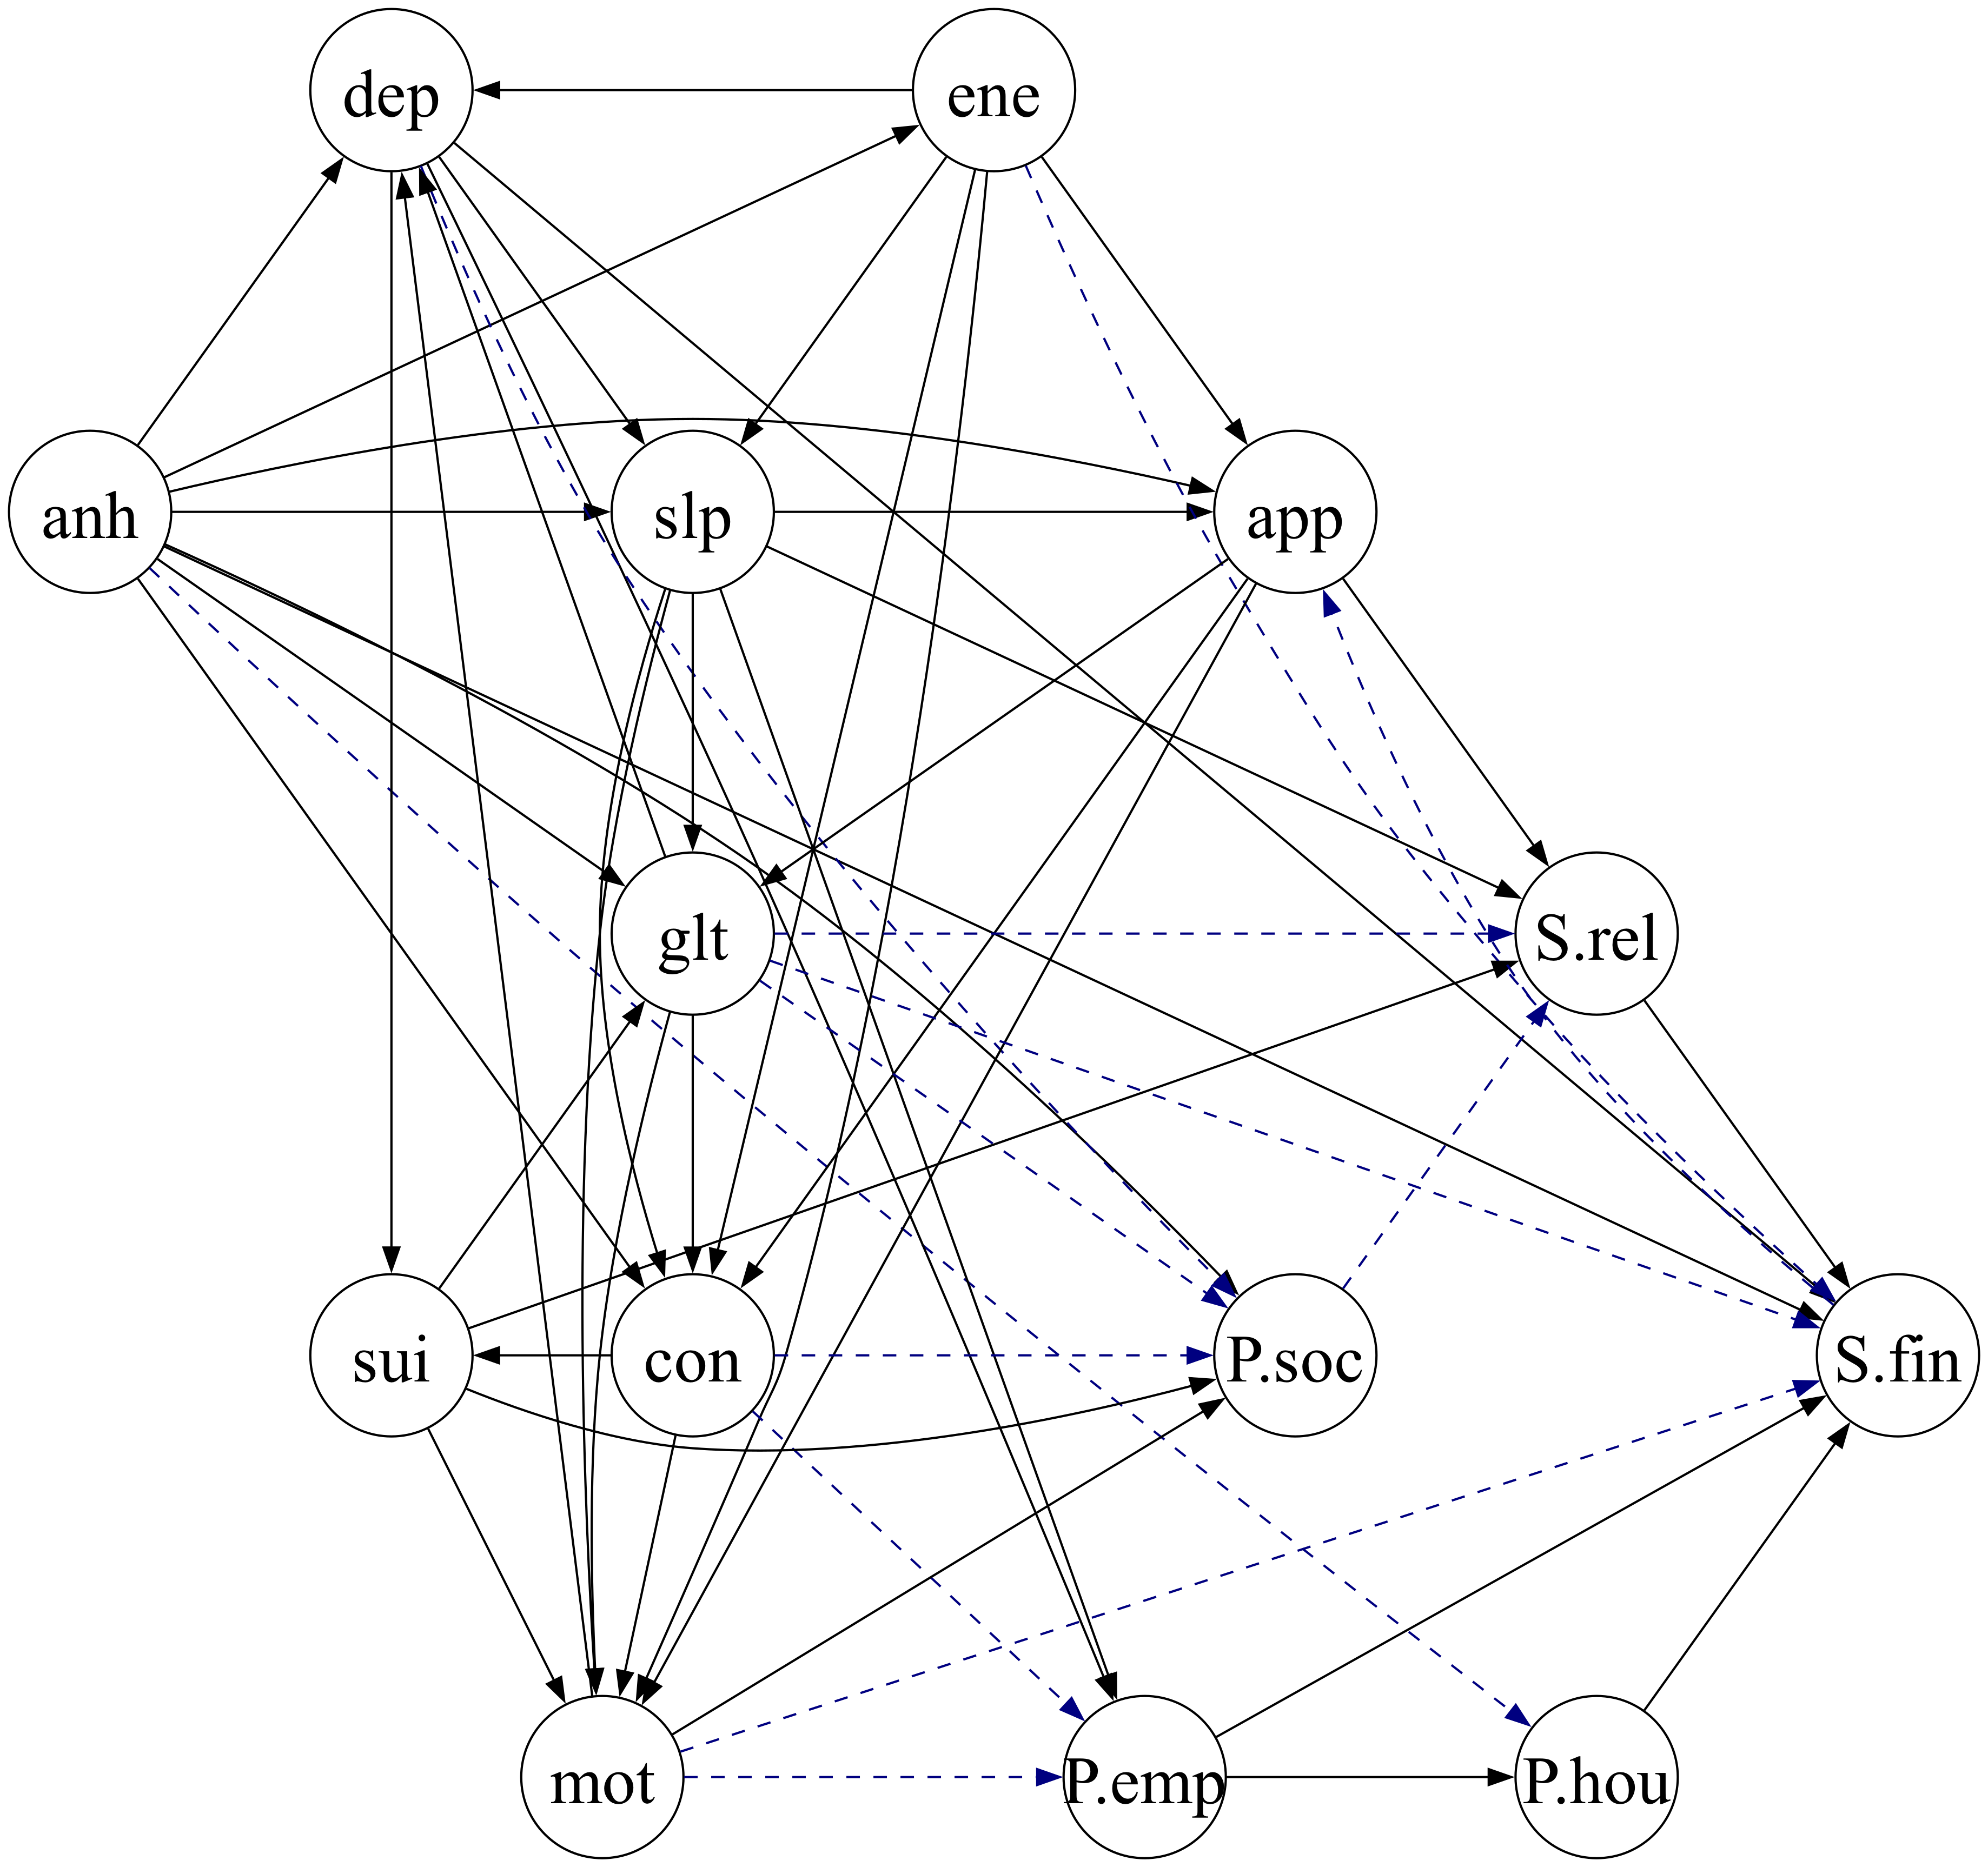
\includegraphics[width=0.6\textwidth,height=\textheight]{img/PC_symptom.png}

}

\caption{\label{fig-pc_sym}\textbf{\emph{Causal pathways linking
individual depressive symptoms and precariousness factors, estimated
with PC.}} The CPDAG representation is denser than FCI or CCI outputs.
Gaussian CI again produces more edges than RCoT (dashed navy edges mark
those unique to Gaussian).}

\end{figure}%

\begin{figure}

\centering{

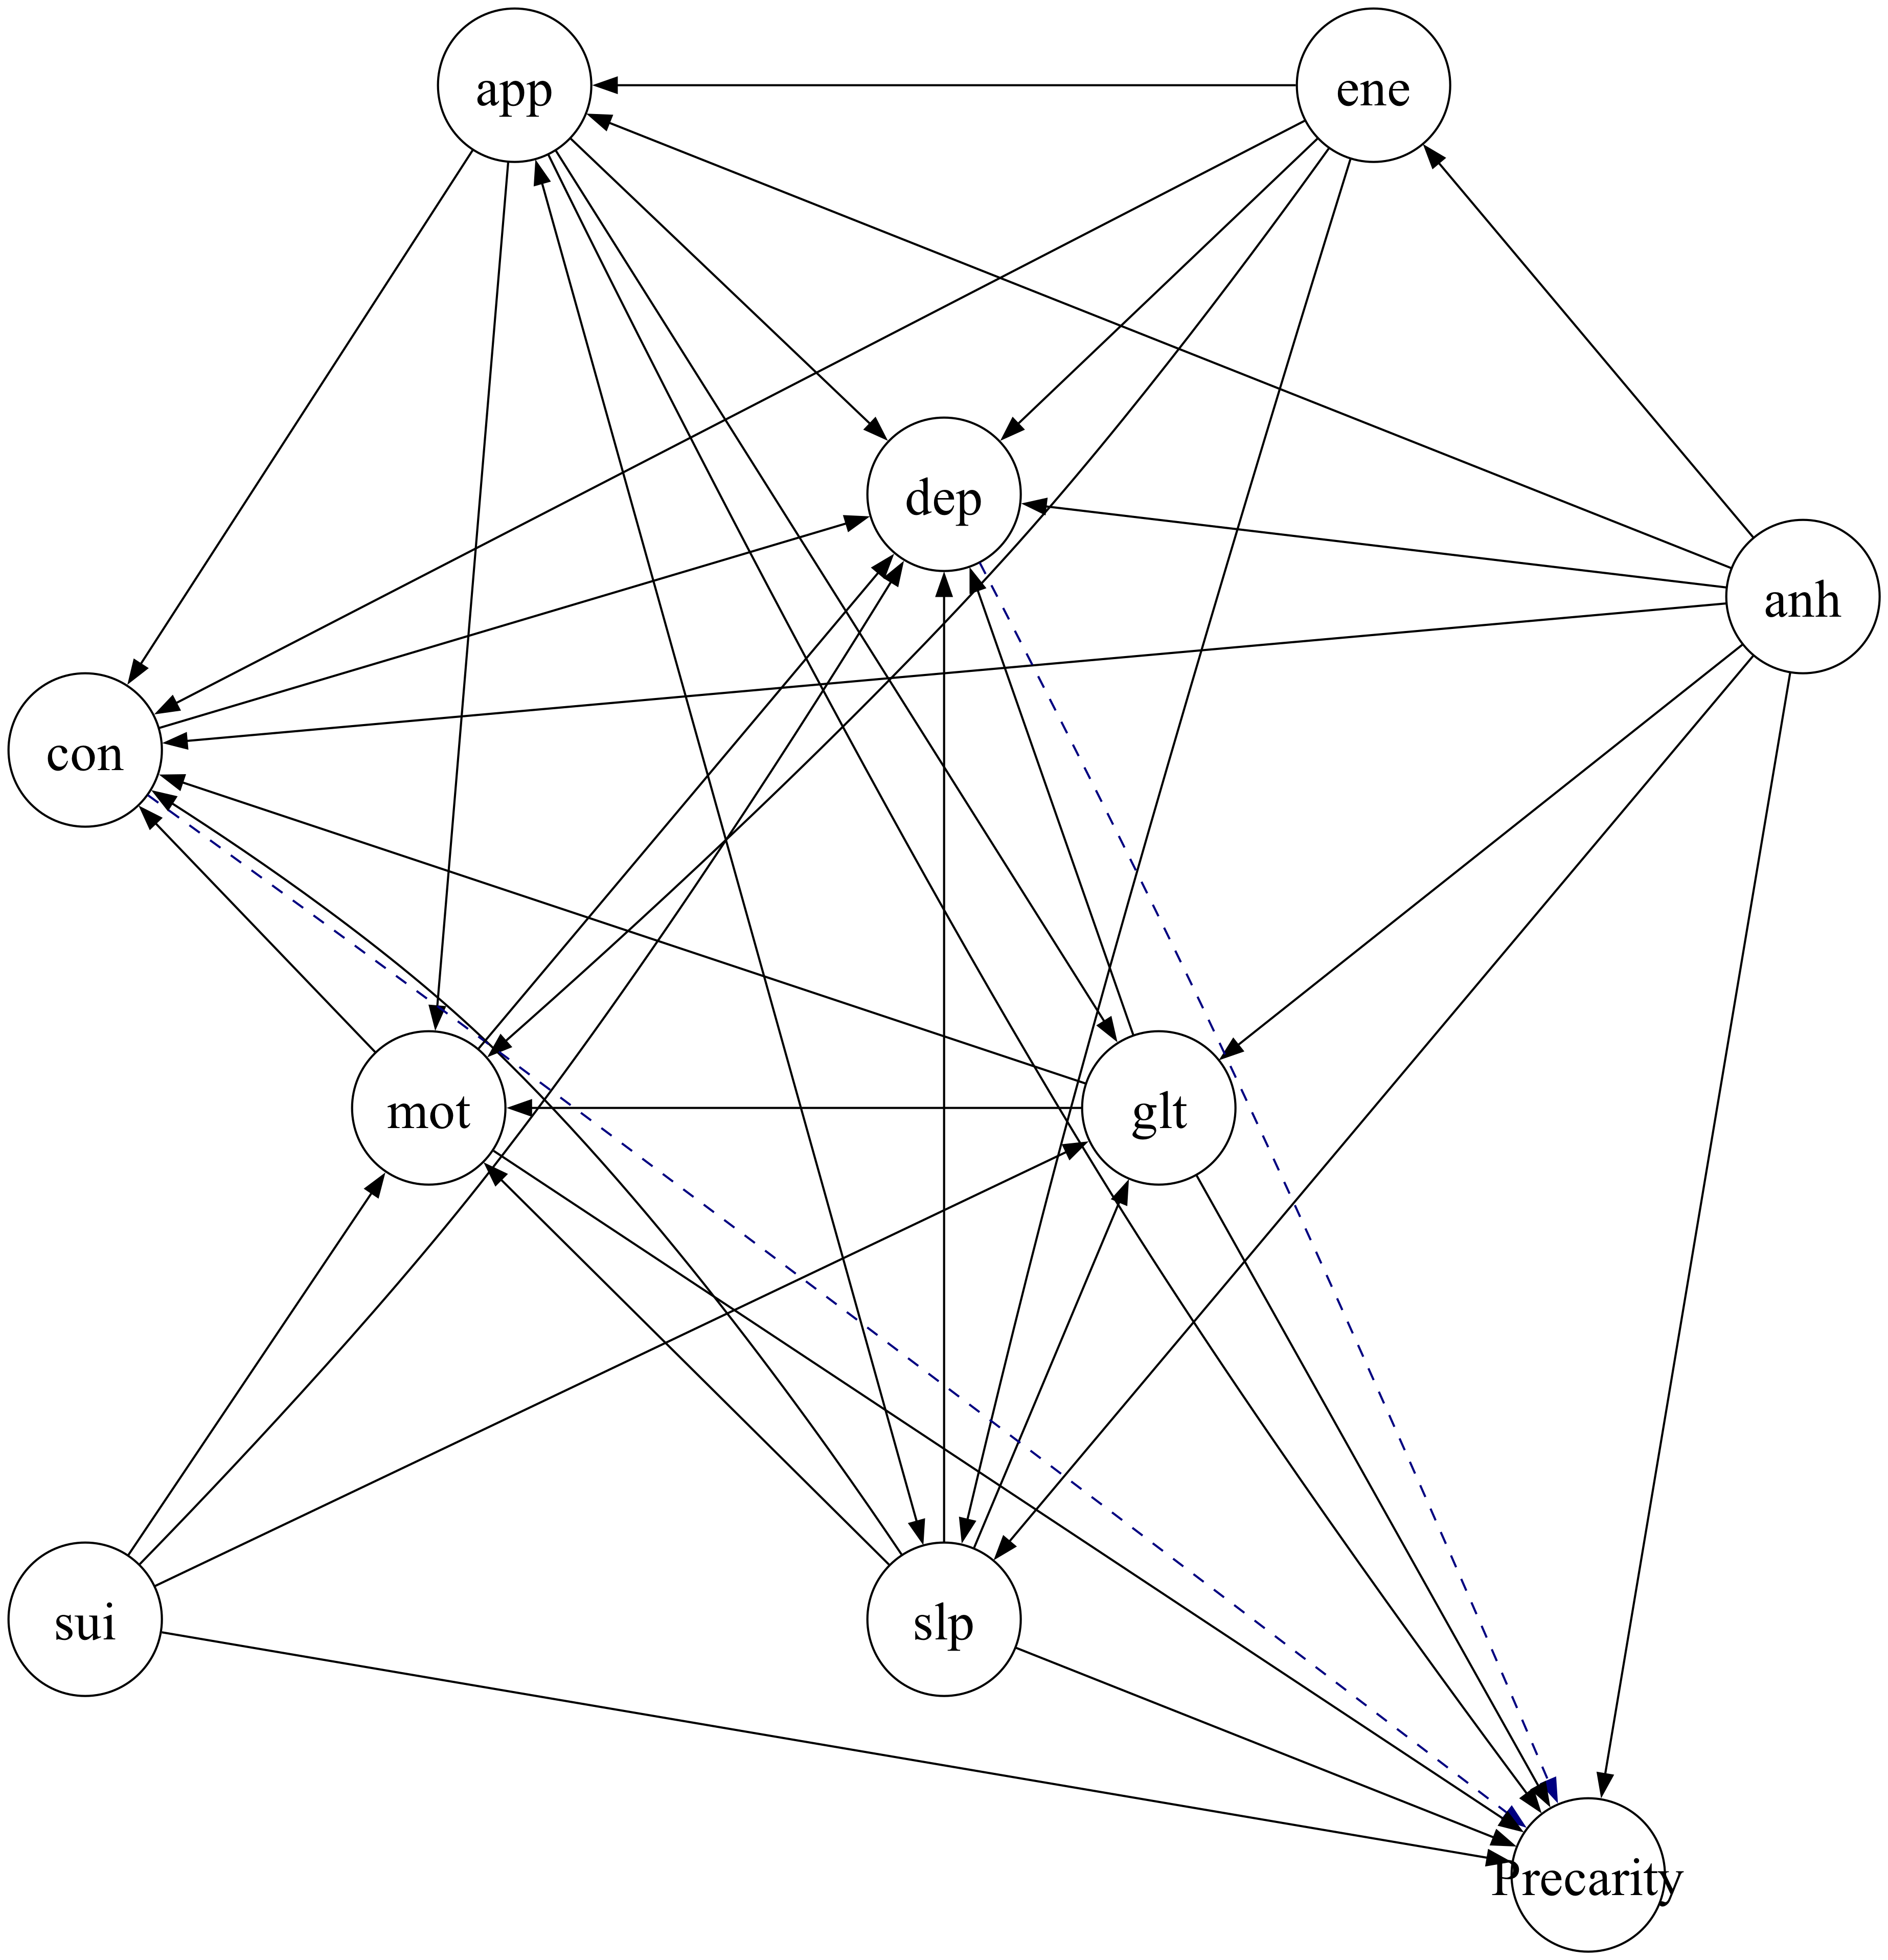
\includegraphics[width=0.6\textwidth,height=\textheight]{img/PC_presum.png}

}

\caption{\label{fig-pc_presum}\textbf{\emph{Causal pathways between
overall precariousness and individual depressive symptoms, estimated
with PC.}} As with the symptom-level graph, PC recovers dense structures
under Gaussian CI but sparser ones under RCoT (dashed navy edges mark
those unique to Gaussian).}

\end{figure}%

\clearpage

\subsection{Randomized Conditional Independence / Correlation Test (RCIT
\& RCoT)}\label{sec-rcot}

RCIT (Randomized Conditional Independence Test) and RCoT (Randomized
conditional Correlation Test) are advanced methods for scalable
conditional independence (CI) testing, offering computational efficiency
while maintaining the accuracy of kernel-based approaches. These methods
evaluate conditional independence between two variables \(X\) and \(Y\)
given a third variable \(Z\) while addressing computational challenges
inherent in kernel-based CI tests. In this section, we provide a
high-level overview of RCIT and RCoT based on (Strobl et al., 2019).

\subsubsection{Kernel-Based Conditional Independence
Testing}\label{kernel-based-conditional-independence-testing}

Traditional kernel-based CI tests, such as the Kernel Conditional
Independence Test (KCIT), compute dependencies using the Hilbert-Schmidt
Independence Criterion (HSIC) in reproducing kernel Hilbert spaces
(RKHS) (Zhang et al., 2011). KCIT uses the following hypothesis
framework: \[
H_0: X \perp\!\!\!\perp Y \,|\, Z, \quad H_1: X \not\!\perp\!\!\!\perp Y \,|\, Z.
\] The core quantity in KCIT is the partial cross-covariance operator:
\[
\Sigma_{XY \cdot Z} = \Sigma_{XY} - \Sigma_{XZ} \Sigma_{ZZ}^{-1} \Sigma_{ZY},
\] where \(\Sigma_{XY}\) represents the cross-covariance operator
between \(X\) and \(Y\), and
\(\Sigma_{XZ} \Sigma_{ZZ}^{-1} \Sigma_{ZY}\) removes the dependence
mediated by \(Z\).

The squared Hilbert-Schmidt (HS) norm of \(\Sigma_{XY \cdot Z}\) serves
as the test statistic: \[
\|\Sigma_{XY \cdot Z}\|^2_{HS} = 0 \quad \text{if and only if} \quad X \perp\!\!\!\perp Y \,|\, Z.
\]

KCIT estimates residual dependencies using kernel ridge regression: \[
f^*(z) = K_Z (K_Z + \lambda I)^{-1} f(x),
\] where \(K_Z\) is the kernel matrix for \(Z\), \(f(x)\) is the kernel
feature map for \(X\), and \(\lambda\) is the ridge regularization
parameter. The residual function for \(X\) is: \[
f_\text{res}(x) = f(x) - f^*(z) = R_Z f(x),
\] with: \[
R_Z = I - K_Z (K_Z + \lambda I)^{-1}.
\] The kernel matrix for residualized \(X\) is: \[
K_{X \cdot Z} = R_Z K_X R_Z,
\] and similarly for \(Y\), \(K_{Y \cdot Z} = R_Z K_Y R_Z\).

The test statistic is computed as: \[
T_{XY \cdot Z} = \frac{1}{n^2} \text{tr}(K_{X \cdot Z} K_{Y \cdot Z}),
\] which estimates the Hilbert-Schmidt (HS) norm of the partial
cross-covariance operator. To ensure convergence, KCIT scales the
statistic by \(n\): \[
S_K = n T_{XY \cdot Z}.
\] The null hypothesis \(H_0\) is rejected if \(S_K\) exceeds a
threshold determined by permutation or moment-matching-based null
distribution (Lindsay et al., 2000).

\subsubsection{Random Fourier Features
(RFFs)}\label{random-fourier-features-rffs}

Kernel-based methods like KCIT face scalability issues, as they involve
operations on \(n \times n\) kernel matrices, which scale quadratically
with the sample size \(n\). RCIT and RCoT overcome this bottleneck using
\emph{Random Fourier Features (RFFs)} to approximate kernel operations
efficiently.

\paragraph{Bochner's Theorem}\label{bochners-theorem}

Bochner's theorem provides the foundation for RFFs, stating that any
continuous shift-invariant kernel \(k(x, y)\) can be expressed as: \[
k(x, y) = \int_{\mathbb{R}^p} e^{i \omega^\top (x - y)} \, dP_\omega,
\] where \(P_\omega\) is the spectral distribution of the kernel. For
the widely used RBF kernel: \[
k(x, y) = \exp\left(-\frac{\|x - y\|^2}{2\sigma^2}\right),
\] \(P_\omega\) follows a Gaussian distribution:
\(\omega \sim \mathcal{N}(0, \sigma^2 I)\).

\paragraph{RFF Approximation}\label{rff-approximation}

Using Monte Carlo sampling, the kernel function is approximated as: \[
k(x, y) \approx \phi(x)^\top \phi(y),
\] where \(\phi(x)\) is the random Fourier feature mapping: \[
\phi(x) = \sqrt{\frac{2}{D}} \cos(W^\top x + b),
\] with \(W \sim \mathcal{N}(0, \sigma^2 I)\) and
\(b \sim \text{Uniform}(0, 2\pi)\). Here, \(D\) is the number of Fourier
features, which balances computational efficiency and approximation
accuracy.

\subsubsection{Differences Between RCIT and
RCoT}\label{differences-between-rcit-and-rcot}

RCIT and RCoT differ in their test statistics, computational efficiency,
and practical performance, which makes them suited for different
scenarios in causal discovery. RCIT evaluates the Hilbert-Schmidt norm
of the full partial cross-covariance operator, providing a general test
for conditional independence but at a higher computational cost. RCoT
simplifies the process by using the Frobenius norm of a
finite-dimensional residualized cross-covariance matrix, significantly
reducing complexity and improving scalability.

These distinctions are particularly important for large-scale datasets,
where RCoT's computational efficiency makes it a practical choice for
high-dimensional causal discovery tasks.
\textcolor{BrickRed}{In our study, we use RCoT primarily for computational scalability at the HELIUS sample size and as part of our sensitivity analyses; it does not remove the fundamental loss of statistical power and increased estimation difficulty that typically occurs as the conditioning set $|Z|$ grows.}

\paragraph{RCIT: Randomized Conditional Independence
Test}\label{rcit-randomized-conditional-independence-test}

RCIT tests full conditional independence by examining the squared
Hilbert-Schmidt (HS) norm of the partial cross-covariance operator
\(\Sigma_{XY \cdot Z}\): \[
S_K = n T_{XY \cdot Z} = \frac{1}{n} \text{tr}(K_{X \cdot Z} K_{Y \cdot Z}),
\] where \(T_{XY \cdot Z}\) is an empirical estimate of
\(\|\Sigma_{XY \cdot Z}\|^2_{HS}\). The null and alternative hypotheses
are: \[
H_0: \|\Sigma_{XY \cdot Z}\|^2_{HS} = 0, \quad H_1: \|\Sigma_{XY \cdot Z}\|^2_{HS} > 0.
\]

RCIT is a general test for conditional independence but becomes
computationally demanding as the size of \(Z\) increases, due to the
high-dimensional kernel operations required.

\paragraph{RCoT: Randomized Conditional Correlation
Test}\label{rcot-randomized-conditional-correlation-test}

RCoT simplifies the testing process by using a finite-dimensional
partial cross-covariance matrix, avoiding full HS norm calculations.
Instead, it uses the Frobenius norm of the residualized cross-covariance
matrix: \[
S' = n \|C_{AB \cdot C}\|_F^2,
\] where \(C_{AB \cdot C}\) represents the residualized cross-covariance
matrix. The hypotheses are: \[
H_0: \|C_{AB \cdot C}\|_F^2 = 0, \quad H_1: \|C_{AB \cdot C}\|_F^2 > 0.
\]

\textcolor{BrickRed}{RCoT is computationally efficient and therefore computationally feasible for larger conditioning sets (relative to KCIT), because it approximates kernel operations via random Fourier features.
However, computational feasibility should not be conflated with statistical suitability: as the conditioning dimension increases, conditional-independence tests—parametric or nonparametric—typically lose power and become more sensitive to model misspecification and measurement error. For this reason, in our application we interpret results involving larger conditioning sets cautiously and emphasize stability/indeterminacy across resampling and specification choices rather than treating orientations as definitive.}

\subsection{Analytical Calibration of the Linear Feedback
Model}\label{sec-analcalibration}

We consider a continuous-time, linear stochastic differential equation
(SDE) model describing the coupled dynamics between depression (\(D\))
and social precariousness (\(P\)), each influenced by an external
stressor (\(S\)). The system is specified as:

\[
\begin{aligned}
\frac{dD}{dt} &= \alpha_{DS} S + \alpha_{DP} P - D + \sigma_D \cdot \eta_D(t), \\
\frac{dP}{dt} &= \alpha_{PS} S + \alpha_{PD} D - P + \sigma_P \cdot \eta_P(t),
\end{aligned}
\]

where:

\begin{itemize}
\tightlist
\item
  \(S\) is a fixed or exogenous input (external financial stress),
\item
  \(\alpha_{DP}\) represents the feedback from precariousness to
  depression,
\item
  \(\alpha_{PD}\) represents the feedback from depression to
  precariousness,
\item
  \(\alpha_{DS}\) and \(\alpha_{PS}\) capture the direct effects of
  \(S\),
\item
  \(\sigma_D, \sigma_P\) are stochastic noise amplitudes,
\item
  \(\eta_D(t), \eta_P(t)\) are independent standard Wiener processes.
\end{itemize}

We fix the decay rates \(\lambda_D = \lambda_P = 1\), normalizing the
time scale due to lack of temporal resolution in the HELIUS dataset.

\subsubsection{Stationarity Assumption}\label{stationarity-assumption}

We assume the joint distribution of \((D, P)\) reaches stationarity,
leading to a multivariate Ornstein--Uhlenbeck process. Under this
assumption, the system has a unique stationary distribution
characterized by its covariance structure, which we match to the
empirical data.

Let:

\[
\Sigma_{DD} = \mathrm{Var}(D), \quad \Sigma_{PP} = \mathrm{Var}(P), \quad \Sigma_{SS} = \mathrm{Var}(S),
\]

\[
\Sigma_{DP} = \mathrm{Cov}(D, P), \quad \Sigma_{DS} = \mathrm{Cov}(D, S), \quad \Sigma_{PS} = \mathrm{Cov}(P, S).
\]

From the HELIUS data, we use the following observed values:

\(\Sigma_{DD} = 1.000, \quad \Sigma_{PP} = 0.807, \quad \Sigma_{SS} = 0.743, \quad \Sigma_{DP} = 0.374, \quad \Sigma_{DS} = 0.357, \quad \Sigma_{PS} = 0.256.\)

\subsubsection{Analytical Parameter
Derivation}\label{analytical-parameter-derivation}

We consider a linear stochastic dynamical system in which depression
(\(D\)) and social precariousness (\(P\)) evolve under mutual influence
and are jointly affected by an exogenous stressor (\(S\)). We assume
stationary dynamics governed by a two-dimensional Ornstein--Uhlenbeck
process:

\[
\begin{aligned}
dD_t &= \left(-D_t + \alpha_{DP} P_t + \alpha_{DS} S_t\right)dt + \sigma_D\, dW_{1t}, \\
dP_t &= \left(-P_t + \alpha_{PD} D_t + \alpha_{PS} S_t\right)dt + \sigma_P\, dW_{2t}.
\end{aligned}
\]

Here, we fix the autoregressive decay rates to 1 for identifiability and
treat \(\alpha_{DP}\) --- the influence of precariousness on depression
--- as a free parameter. All other parameters are then derived to ensure
the model reproduces the empirical second-order moments: variances
\((\Sigma_{DD}, \Sigma_{PP}, \Sigma_{SS})\) and covariances
\((\Sigma_{DP}, \Sigma_{DS}, \Sigma_{PS})\).

Under the stationary solution of the linear SDE system, the following
algebraic identities hold:

\[
\begin{aligned}
\Sigma_{DS} &= \alpha_{DS} \Sigma_{SS} + \alpha_{DP} \Sigma_{PS}, \\
\Sigma_{DP} &= \alpha_{DS} \Sigma_{PS} + \alpha_{DP} \Sigma_{PP}, \\
\Sigma_{PS} &= \alpha_{PS} \Sigma_{SS} + \alpha_{PD} \Sigma_{DS}.
\end{aligned}
\]

Solving these simultaneously yields the following closed-form
expressions as functions of \(\alpha_{DP}\):

\[
\alpha_{DS} = \frac{\Sigma_{DS} - \alpha_{DP} \cdot \Sigma_{PS}}{\Sigma_{SS}},
\]

\[
\alpha_{PD} = \frac{2 \Sigma_{DS} \Sigma_{PS} - 2 \Sigma_{DP} \Sigma_{SS} - \alpha_{DP} \Sigma_{PS}^2 + \alpha_{DP} \Sigma_{PP} \Sigma_{SS}}{\Sigma_{DS}^2 - \Sigma_{DD} \Sigma_{SS}},
\]

\[
\alpha_{PS} = \frac{
\Sigma_{DS}^2 \Sigma_{PS}
+ \Sigma_{PS} \Sigma_{DD} \Sigma_{SS}
+ \Sigma_{DS}(-2 \Sigma_{DP} \Sigma_{SS} - \alpha_{DP} \Sigma_{PS}^2 + \alpha_{DP} \Sigma_{PP} \Sigma_{SS})
}{
\Sigma_{SS}(\Sigma_{DS}^2 - \Sigma_{DD} \Sigma_{SS})
}.
\]

The noise amplitudes \(\sigma_D^2\) and \(\sigma_P^2\) are derived from
the Lyapunov equation associated with the stationary covariance matrix.
These yield:

\[
\sigma_D^2 = \frac{-2 \left(\Sigma_{DS}^2 - \Sigma_{DD} \Sigma_{SS} - \Sigma_{DS} \Sigma_{PS} \alpha_{DP} + \Sigma_{DP} \Sigma_{SS} \alpha_{DP} \right)}{\Sigma_{SS}},
\]

\[
\sigma_P^2 = \frac{K}{\Sigma_{SS} (\Sigma_{DD} \Sigma_{SS} - \Sigma_{DS}^2)},
\]

where

\[
\begin{aligned}
K &= 8 \Sigma_{DP} \Sigma_{DS} \Sigma_{PS} \Sigma_{SS}
- 4 \Sigma_{DP}^2 \Sigma_{SS}^2
- 2 \Sigma_{DS}^2 (\Sigma_{PS}^2 + \Sigma_{PP} \Sigma_{SS}) \\
&\quad + 2 \Sigma_{DS} \Sigma_{PS} (\Sigma_{PS}^2 - \Sigma_{PP} \Sigma_{SS}) \alpha_{DP}
+ 2 \Sigma_{SS} (\Sigma_{PP} \Sigma_{SS} - \Sigma_{PS}^2)(\Sigma_{DD} + \Sigma_{DP} \alpha_{DP}).
\end{aligned}
\]

These expressions define a one-parameter family of structurally distinct
yet observationally equivalent models, each exactly matching the
empirical second-order statistics.

\subsubsection{\texorpdfstring{Constraints on
\(\alpha_{DP}\)}{Constraints on \textbackslash alpha\_\{DP\}}}\label{constraints-on-alpha_dp}

Although all expressions are algebraically valid for arbitrary real
\(\alpha_{DP}\), admissibility requires that the resulting model remains
meaningful and stable.

\paragraph{Positivity Constraints}\label{positivity-constraints}

To ensure interpretability, we require all effects and noise terms to be
strictly positive:

\[
\alpha_{DS} > 0, \quad \alpha_{PD} > 0, \quad \alpha_{PS} > 0, \quad \sigma_D^2 > 0, \quad \sigma_P^2 > 0.
\]

Each of these is a function of \(\alpha_{DP}\), and thus these
conditions restrict its allowable range. In particular:

\begin{itemize}
\tightlist
\item
  \(\alpha_{PD} = 0\) when \(\alpha_{DP} \approx 0.698\),
\item
  \(\alpha_{DS} = 0\) when \(\alpha_{DP} \approx 1.39\),
\item
  \(\sigma_D^2 = 0\) when \(\alpha_{DP} \approx 3.30\),
\item
  \(\sigma_P^2 = 0\) at a value given exactly by:
\end{itemize}

\[
\alpha_{DP}^{(\sigma_P = 0)} =
\frac{
- \Sigma_{DD} \Sigma_{PP} \Sigma_{SS}^2 + \Sigma_{DD} \Sigma_{PS}^2 \Sigma_{SS}
+ 2 \Sigma_{DP}^2 \Sigma_{SS}^2 - 4 \Sigma_{DP} \Sigma_{DS} \Sigma_{PS} \Sigma_{SS}
+ \Sigma_{DS}^2 \Sigma_{PP} \Sigma_{SS} + \Sigma_{DS}^2 \Sigma_{PS}^2
}{
\Sigma_{DP} \Sigma_{PP} \Sigma_{SS}^2 - \Sigma_{DP} \Sigma_{PS}^2 \Sigma_{SS}
- \Sigma_{DS} \Sigma_{PP} \Sigma_{PS} \Sigma_{SS} + \Sigma_{DS} \Sigma_{PS}^3
}.
\]

This value falls above \(\alpha_{DP} = 0.698\), and thus does not
tighten the admissible upper bound.

\paragraph{Stability Constraint}\label{stability-constraint}

The system is stable if the deterministic dynamics converge, which
requires the drift matrix

\[
A = \begin{bmatrix}
-1 & \alpha_{DP} \\
\alpha_{PD} & -1
\end{bmatrix}
\]

to have all eigenvalues with negative real parts. This is equivalent to:

\[
\text{Tr}(A) < 0 \quad \text{and} \quad \det(A) = 1 - \alpha_{DP} \alpha_{PD} > 0.
\]

The trace condition is always satisfied (\(\text{Tr}(A) = -2\)), so
stability reduces to:

\[
\alpha_{DP} \cdot \alpha_{PD} < 1.
\]

This condition fails exactly when \(\alpha_{PD} \to 0^+\), which
coincides with the tightest positivity constraint.

\subsubsection{Admissible Range}\label{admissible-range}

Numerical evaluation using empirical covariances from the HELIUS dataset
shows that:

\begin{itemize}
\tightlist
\item
  \(\alpha_{PD} \to 0\) at \(\alpha_{DP} \approx 0.698\),
\item
  All other positivity and stability constraints are looser.
\end{itemize}

Hence, the maximum valid value is:

\[
\boxed{\alpha_{DP}^{\max} = 0.698}
\]

All simulations and model variants are confined to the admissible
domain:

\[
\alpha_{DP} \in [0,\, 0.698]
\]

This guarantees that resulting systems are dynamically stable, fully
positive, and consistent with empirical second-order moments.




\end{document}
